% sample.tex
\documentclass[8pt,xcolor=svgnames]{beamer} 
\setlength{\parindent}{0pt}
\setlength{\parskip}{1.5ex}

\usepackage{mathptmx}
\usepackage{helvet}
\usepackage{hyperref}
\usepackage{animate}

\usefonttheme[onlymath]{serif}
\usecolortheme[named=DarkGreen]{structure}
\useoutertheme{infolines} 
\usetheme[height=7mm]{Rochester} 
\hypersetup{colorlinks=true,linkcolor=red} 
\setbeamertemplate{items}[ball] 
\setbeamertemplate{blocks}[rounded][shadow=true] 
\setbeamertemplate{navigation symbols}{} 

% items enclosed in square brackets are optional; explanation below
\title[High Order Finite Elements for Lagrangian CFD]{\LARGE{High Order Finite Elements for Lagrangian \\Computational Fluid Dynamics}}
\author[Truman Ellis]{\LARGE{Truman E. Ellis}\\[1ex]
\small{Advisor: Dr. Faisal Kolkailah\\ LLNL Mentors: Dr. Robert Rieben and Dr. Tzanio Kolev}}
\institute[Cal Poly]{\large{
  Department of Aerospace Engineering\\
  California Polytechnic State University\\
  San Luis Obispo, CA \\[1ex]
  \texttt{ellis.truman@gmail.com}
}}
\date[April 2010]{April 23, 2010}

\begin{document}
%--- the titlepage frame -------------------------%
\begin{frame}[plain]
  \titlepage
  \begin{columns}
   \begin{column}{0.3\textwidth}
   \flushright
    
\includegraphics[height=0.4in]{./Images/llnl_logo.png}
   \end{column}
   \begin{column}{0.3\textwidth}
   \centering
    \tiny{\color{blue}{
      This work performed under the auspices \newline
      of the U.S. Department of Energy by \newline
      Lawrence Livermore National Laboratory \newline
      under Contract DE-AC52-07NA27344 \newline
      LLNL-PRES-416883, -416822
      }}
   \end{column}
   \begin{column}{0.3\textwidth}
   \flushleft
    
\includegraphics[height=0.5in]{./Images/cp_seal.png}
   \end{column}
  \end{columns}
  \smallskip
  \begin{flushright}
   \tiny{Powered by \rmfamily{\LaTeX}}
  \end{flushright}
\end{frame}

%--- the presentation begin here -----------------%
\begin{frame}
 \frametitle{Outline}
\begin{columns}
 \begin{column}{0.4\textwidth}
\begin{itemize}
 \item Introduction
 \begin{itemize}
  \item Frameworks
  \item Overview
 \end{itemize}
 \item Theory
 \begin{itemize}
  \item Euler Equations
  \item Lagrangian Mesh Motion
  \item Finite Element Method
  \item Semi-Discrete Formulation
  \item Methods Considered
  \item Bi-Quadratic Methods
 \end{itemize}
 \item Numerical Results
 \begin{itemize}
  \item Static Momentum Solve
  \item Sod Shock Tube
  \item Acoustic Wave
  \item Noh Implosion
  \item Saltzman Piston
  \item Sedov Explosion
  \item Computational Efficiency
 \end{itemize}
 \item Conclusions
\end{itemize}
 \end{column}

\begin{column}{0.5\textwidth}
 \centering
 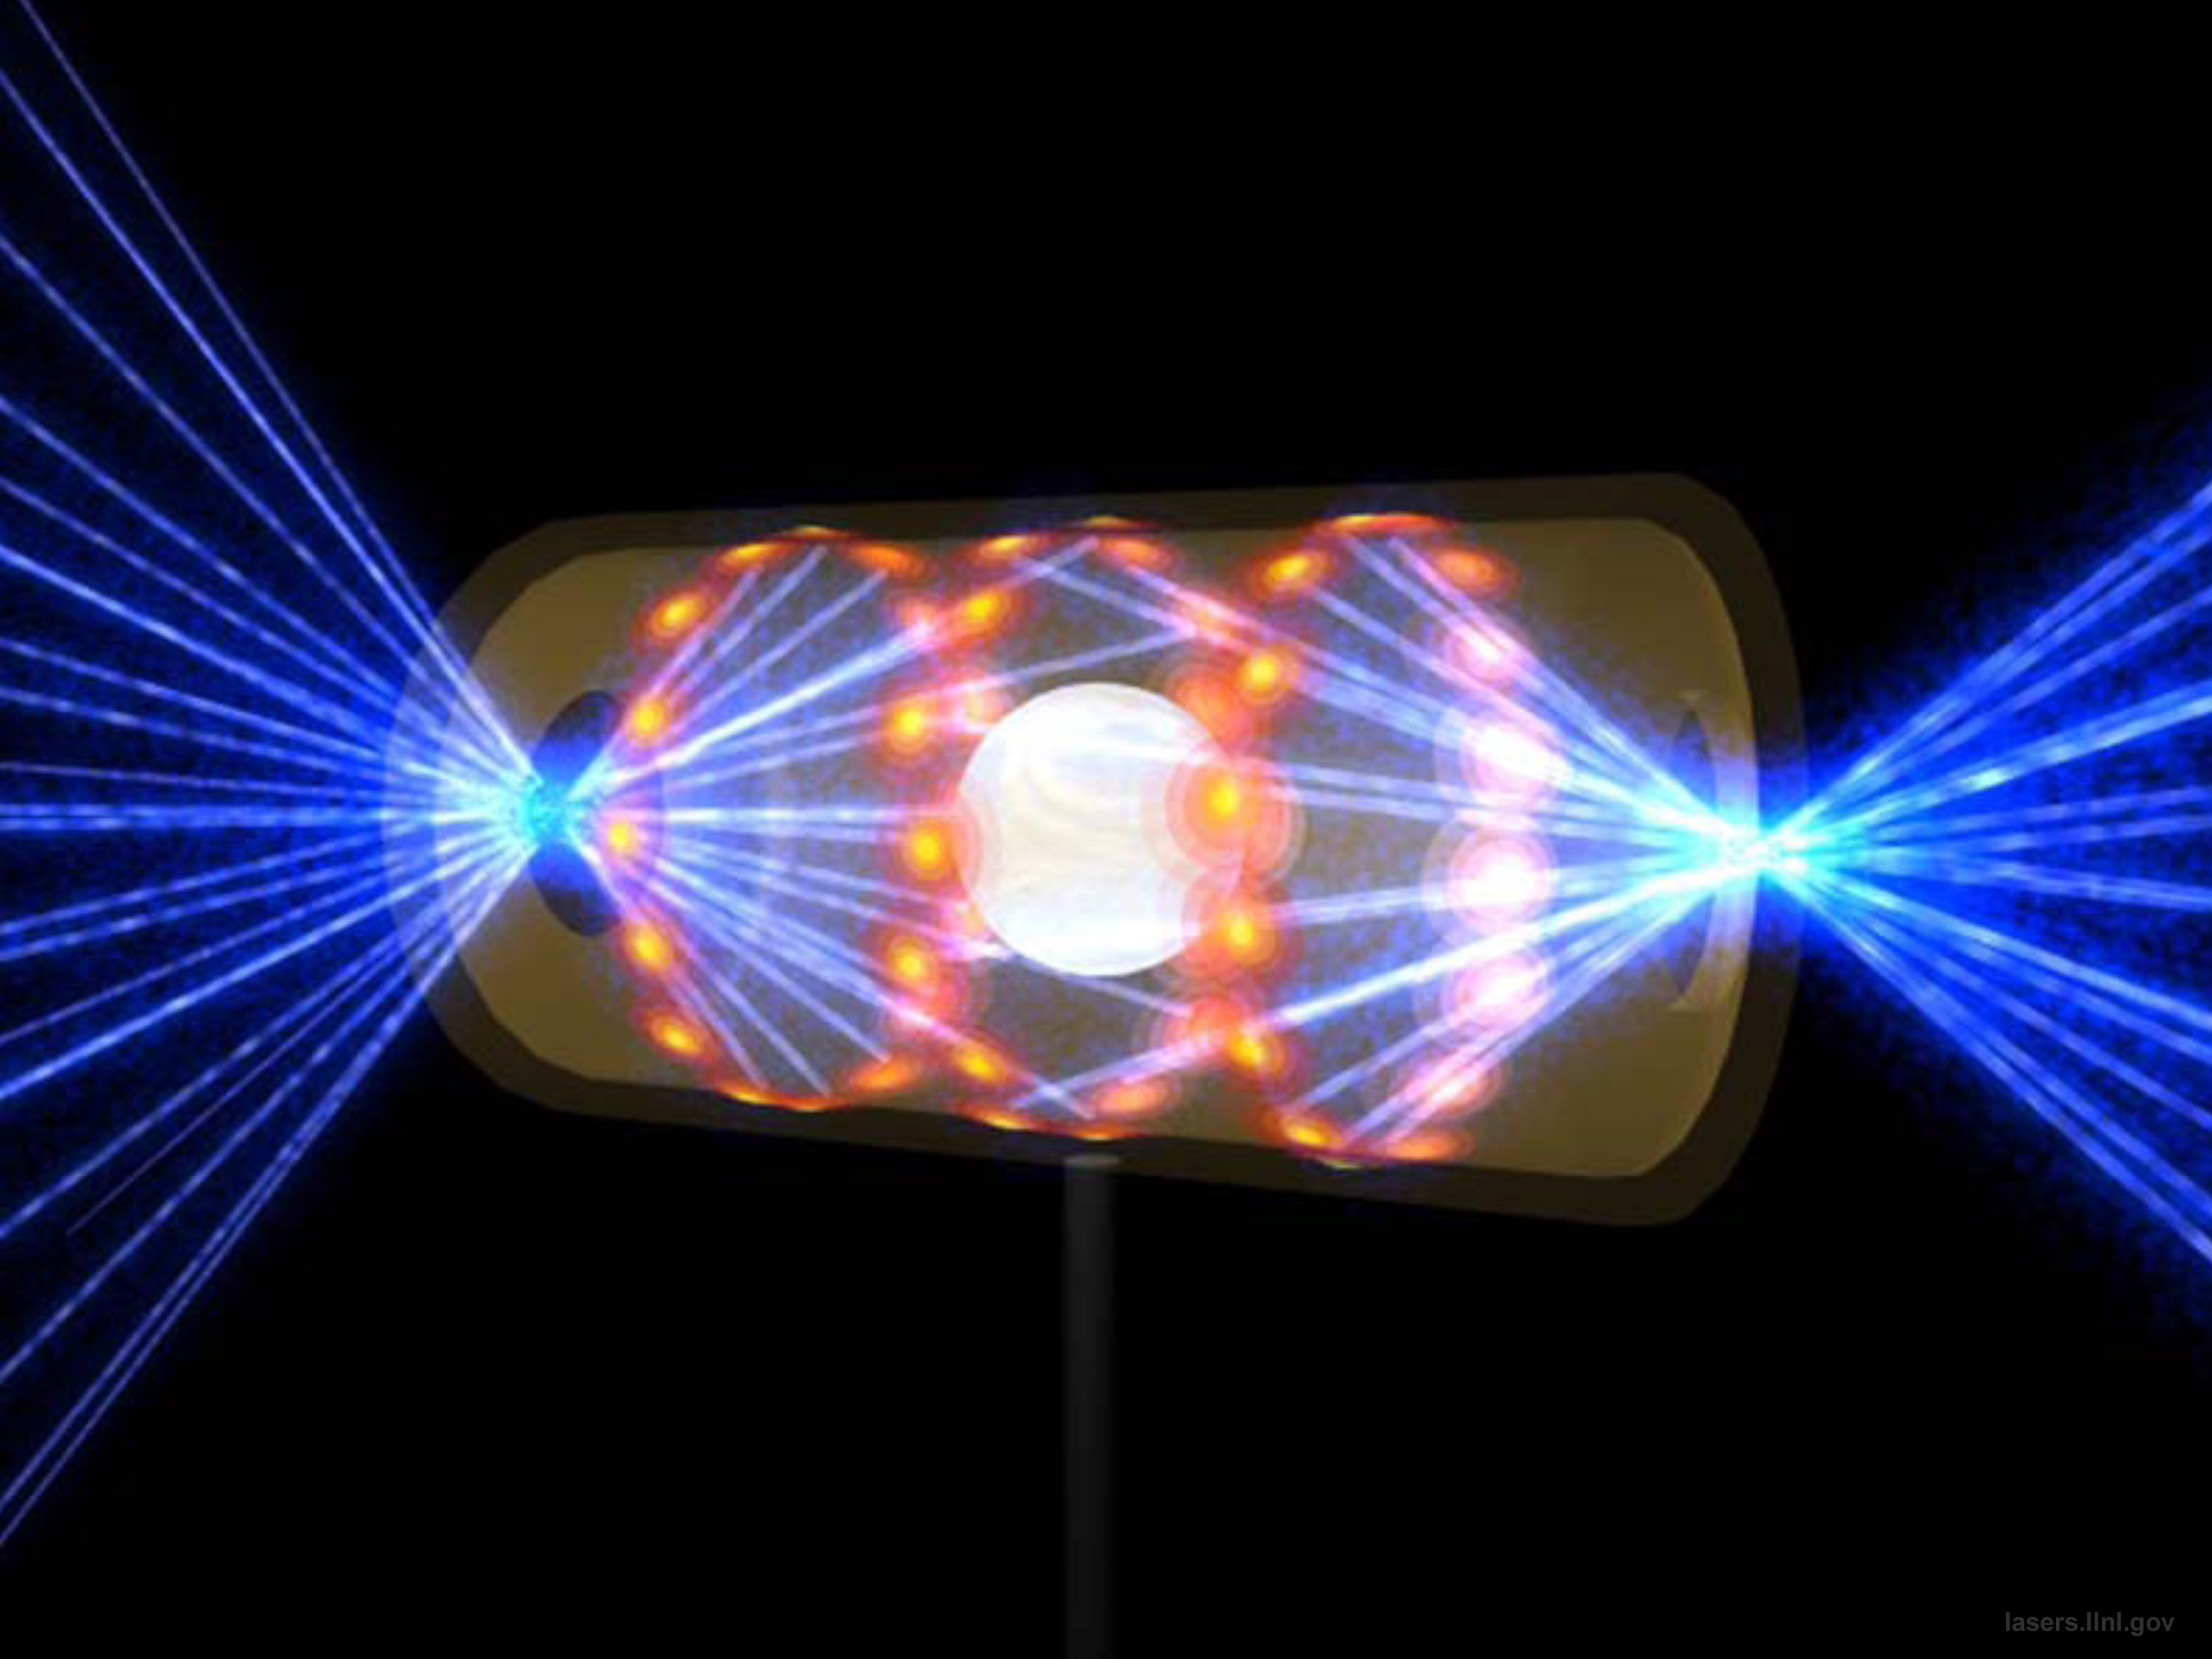
\includegraphics[width=0.8\textwidth,keepaspectratio=true]{./Images/nifcapsule.jpg}

 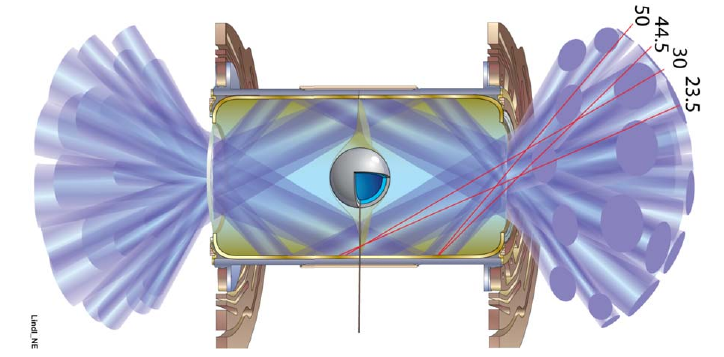
\includegraphics[width=1.0\textwidth,keepaspectratio=true]{./Images/nifIllustration2.png}

 \tiny{courtesy llnl.gov}
\end{column}
\end{columns}



\end{frame}


\begin{frame}
 \frametitle{Frameworks}
\medskip
\begin{block}{Typical simulation frameworks}
\begin{itemize}
 \item Eulerian: Traditional CFD - material is fluxed through a stationary mesh
 \item Lagrangian: Mesh nodes follow material particles - mesh moves with the material
 \item Arbitrary Lagrangian-Eulerian (ALE): Lagrangian until mesh tangling is detected. \\Fluid simulation is paused as the mesh is relaxed. \\
Stationary state variables are advected through the moving mesh.
\end{itemize}
\end{block}
\vspace*{-1ex}
\begin{figure}[h!]
 \centering
 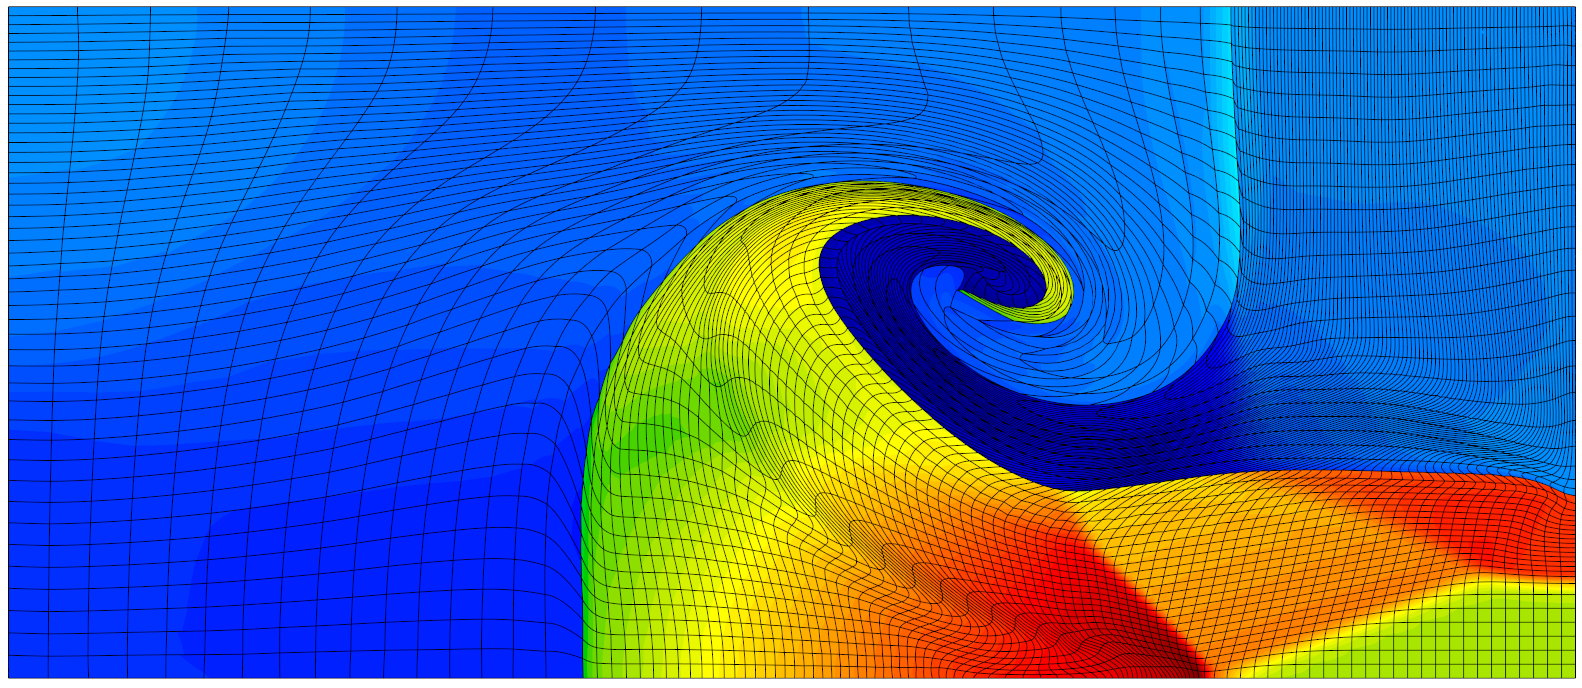
\includegraphics[height=0.55\textheight,keepaspectratio=true]{./Images/triple.png}
\end{figure}
\vspace*{-3ex}
\begin{center}
 Lagrangian simulation of a triple point shock
\end{center}

\end{frame}

% Introduction
\begin{frame}
  \frametitle{Introduction}

\begin{columns}
  \begin{column}{0.6\textwidth}
  \begin{large}
    \begin{itemize}
      \item This thesis develops advanced finite element discretization methods for Lagrangian hydrodynamics.
      \item The goal is to improve the current staggered grid hydro (SGH) algorithms in multi-material ALE codes with respect to:
      \begin{itemize}
	\item symmetry preservation
	\item energy conservation
	\item artificial viscosity discretization
	\item hourglass-mode instabilities
      \end{itemize}
      \item We consider a general framework for solving the Euler equations with the following features:
      \begin{itemize}
	\item allows for high order field representations
	\item allows for curved element geometry
	\item exact energy conservation by construction
	\item reduces to classical SGH under simplifying assumptions
      \end{itemize}
    \end{itemize}
    \end{large}
  \end{column}
  
  \begin{column}{0.4\textwidth}
    \begin{figure}[h!]
 \centering
 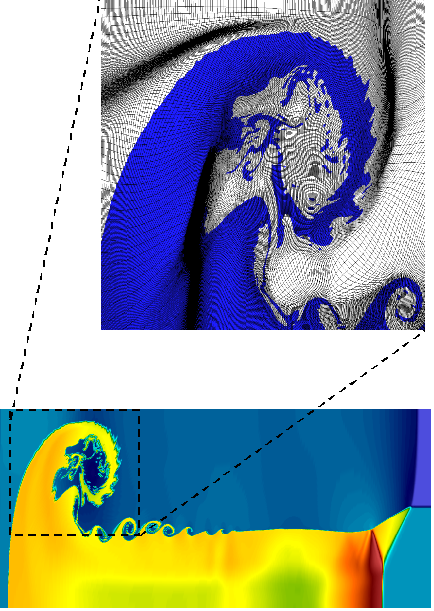
\includegraphics[height=0.8\textheight,keepaspectratio=true]{./Images/lagHydro.png}
 % lagHydro.png: 434x611 pixel, 107dpi, 10.27x14.45 cm, bb=0 0 291 410
\end{figure}
  \end{column}
\end{columns}
\end{frame}

% Outline
\begin{frame}
 \frametitle{Glossary}
 We consider several different hydro methods which make use of various finite element spaces. The specific finite element spaces considered in this talk are:
 \medskip
 \begin{itemize}
  \item Q0: discontinuous constant finite element space on quadrilaterals
  \item Q1: continuous bi-linear finite element space on quadrilaterals
  \item Q2: continuous bi-quadratic finite element space on quadrilaterals
  \item Q1d: discontinuous bi-linear finite element space on quadrilaterals
  \item Q2d: discontinuous bi-quadratic finite element space on quadrilaterals
 \end{itemize}
 \medskip
 Each hydro method is designated by a pair of finite element spaces:
 \medskip
 \begin{itemize}
  \item A continuous kinematic space
  \item A discontinuous thermodynamic space
 \end{itemize}
\begin{center}
\medskip
\begin{block}{For example: }
Q2-Q1d uses continuous quadratic velocities and positions with discontinuous bi-linear pressures and densities. All methods are assumed to have a discontinuous constant energy space.
\end{block}
\end{center}
\end{frame}

% Euler Equations in Lagrangian Frame
\begin{frame}
  \frametitle{Euler Equations in a Lagrangian Frame}
\begin{columns}
  \begin{column}{0.55\textwidth}
    \begin{block}<+->{The Euler equations of gas dynamics in a Lagrangian reference frame can be written in differential form as:}
    \bigskip 
    
\begin{tabular}{ll}
Momentum Conservation: & $\rho \dfrac{\mathrm{d} v}{\mathrm{d} t}=-\vec{\nabla} p + ...$ \\ \\
Mass Conservation: & $\dfrac{1}{\rho}\dfrac{\mathrm{d} \rho}{\mathrm{d} t}=-\vec{\nabla}\cdot \vec{v} $ \\ \\
Energy Conservation: & $\rho \dfrac{\mathrm{d} e}{\mathrm{d} t} =-p\vec{\nabla}\cdot \vec{v} +...$ \\ \\
Equation of State: & $p=EOS(e, \rho)$ \\
\end{tabular}
    \end{block}
  \end{column}
  \begin{column}{0.35\textwidth}
  \bigskip 
  
  Typically, these equations are solved on a staggered spatial grid $^{[1,2]}$ where thermodynamic variables are approximated as piece-wise constants defined on zone centers and kinematic variables are defined on the nodes.
  
\medskip

Spatial gradients are computed using finite volume and/or finite difference methods:
    \begin{figure}[h!]
 \centering
 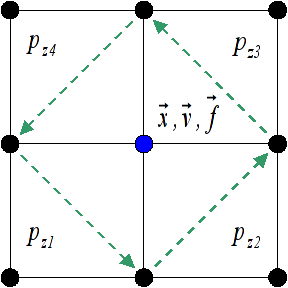
\includegraphics[width=0.6\textwidth,keepaspectratio=true]{./Images/HEMPLagHydro.png}
 % lagHydro.png: 434x611 pixel, 107dpi, 10.27x14.45 cm, bb=0 0 291 410
\end{figure}
  \end{column}
\end{columns}

\tiny{
$^{[1]}$ R. Tipton, “CALE Lagrange Step”, unpublished LLNL report, 1990\newline
$^{[2]}$ M. Wilkins, “Calculations of Elastic-Plastic Flow,” In Methods of Computational Physics, 1964}
\end{frame}

% Semi-Discrete Finite Element Approximation: Computational Mesh
\begin{frame}%[shrink=0]
 \frametitle{Domain Decomposition}
 \medskip
 We propose a general semi-discrete FEM approach to solving the Euler equations in a Lagrangian frame.  A semi-discrete method is only concerned with the spatial approximation of the continuum equations.
 
To begin, we decompose the continuum domain at an initial time into a set of non-overlapping discrete volumes (zones). The union of these volumes forms the computational mesh: 

\begin{columns}
  \begin{column}{0.4\textwidth}
   \begin{figure}[h!]
    \centering
    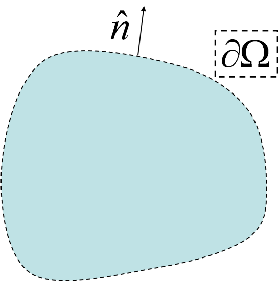
\includegraphics[width=0.6\textwidth,keepaspectratio=true]{./Images/discretization1.png}
    \end{figure}
    \begin{Large}
    \[
     \Omega (t_0)
    \]
    \end{Large}
  \end{column}
  \begin{column}{0.1\textwidth}
   \Huge{$\mathbf{\longrightarrow}$}
  \end{column}
  \begin{column}{0.4\textwidth}
   \begin{figure}[h!]
    \centering
    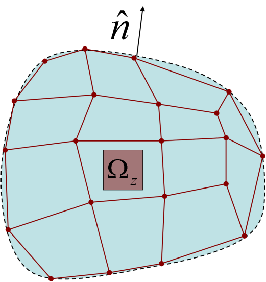
\includegraphics[width=0.6\textwidth,keepaspectratio=true]{./Images/discretization2.png}
    \end{figure}
    \begin{Large}
    \[
     \tilde{\Omega} (t_0)=\bigcup_z \Omega_z(t_0)
    \]
    \end{Large}
  \end{column}
\end{columns}
\vspace*{-4ex}
\begin{center}
\bigskip
\bigskip
\begin{block}{}
The motion of the continuous medium will therefore be described by the motion of only a finite number of particles (mesh vertices, edge midpoints, etc …)
\end{block}
\end{center}
\end{frame}

% Semi-Discrete Finite Element Approximation: Lagrangian Mesh Motion
\begin{frame}
 \frametitle{Lagrangian Mesh Motion}
 \begin{columns}[T]
  \begin{column}{0.65\textwidth}
   After deformation in time, zones are reconstructed based on particle locations, thus defining the moved mesh.
   \begin{columns}
   \begin{column}{0.5\textwidth}
   \begin{figure}[h!]
    \centering
    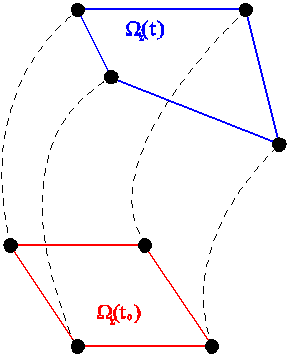
\includegraphics[width=0.9\textwidth,keepaspectratio=true]{./Images/motion1.png}
    \end{figure}
    \centering
    Q1 (Bi-Linear) Approximation
    \end{column}
    \begin{column}{0.5\textwidth}
    \begin{figure}[h!]
    \centering
    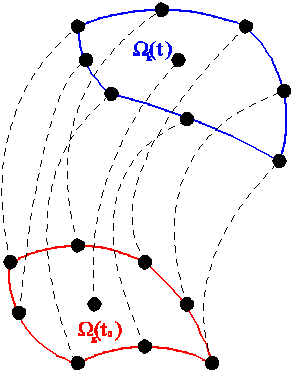
\includegraphics[width=0.9\textwidth,keepaspectratio=true]{./Images/motion2.png}
    \end{figure}
    \centering
    Q2 (Bi-Quadratic) Approximation
    \end{column}
    \end{columns}
  \end{column}
  \begin{column}{0.3\textwidth}
   This reconstruction process has an inherent geometric error.
   \begin{block}{}
    \begin{figure}[h!]
    \centering
    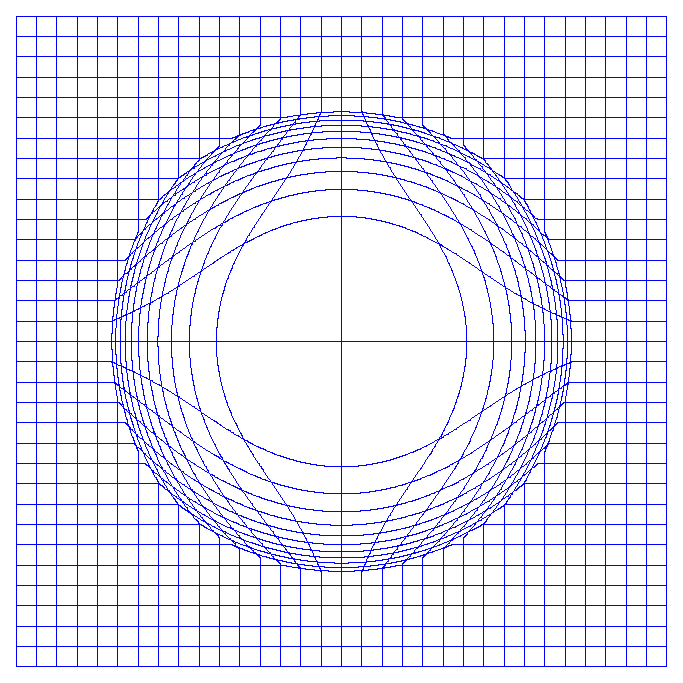
\includegraphics[width=1.0\textwidth,keepaspectratio=true]{./Images/sedovCart.png}
    \end{figure}
    Initial Cartesian mesh deformed with the exact solution of the Sedov blast wave problem. 
   \end{block}
  \end{column}
 \end{columns}
 \begin{block}{}
  This built in geometric error motivates the use of (higher order) finite elements which can use the additional particle degrees of freedom to more accurately represent continuous deformations.
 \end{block}
\end{frame}

% \begin{frame}
%  \frametitle{Lagrangian Mesh Motion: Animation}
% \centering
% \href{run:anSedov.sh}{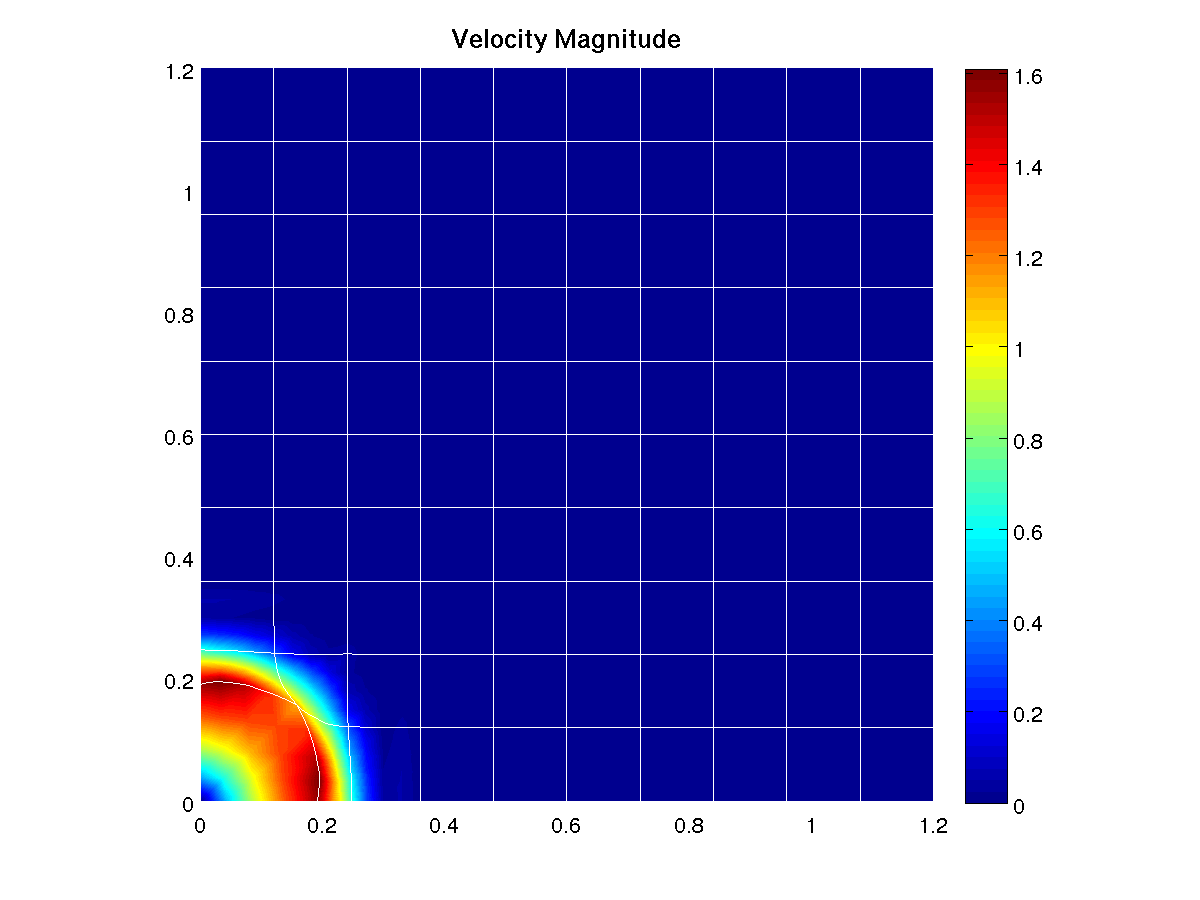
\includegraphics[height=1.0\textheight,keepaspectratio=true]{./Images/SedovAnimation_00.png}}
% \end{frame}


\begin{frame}
 \frametitle{Lagrangian Mesh Motion: Animation} 
\begin{figure}[ht]
\begin{animateinline}[autoplay,width=\textwidth]{1}
    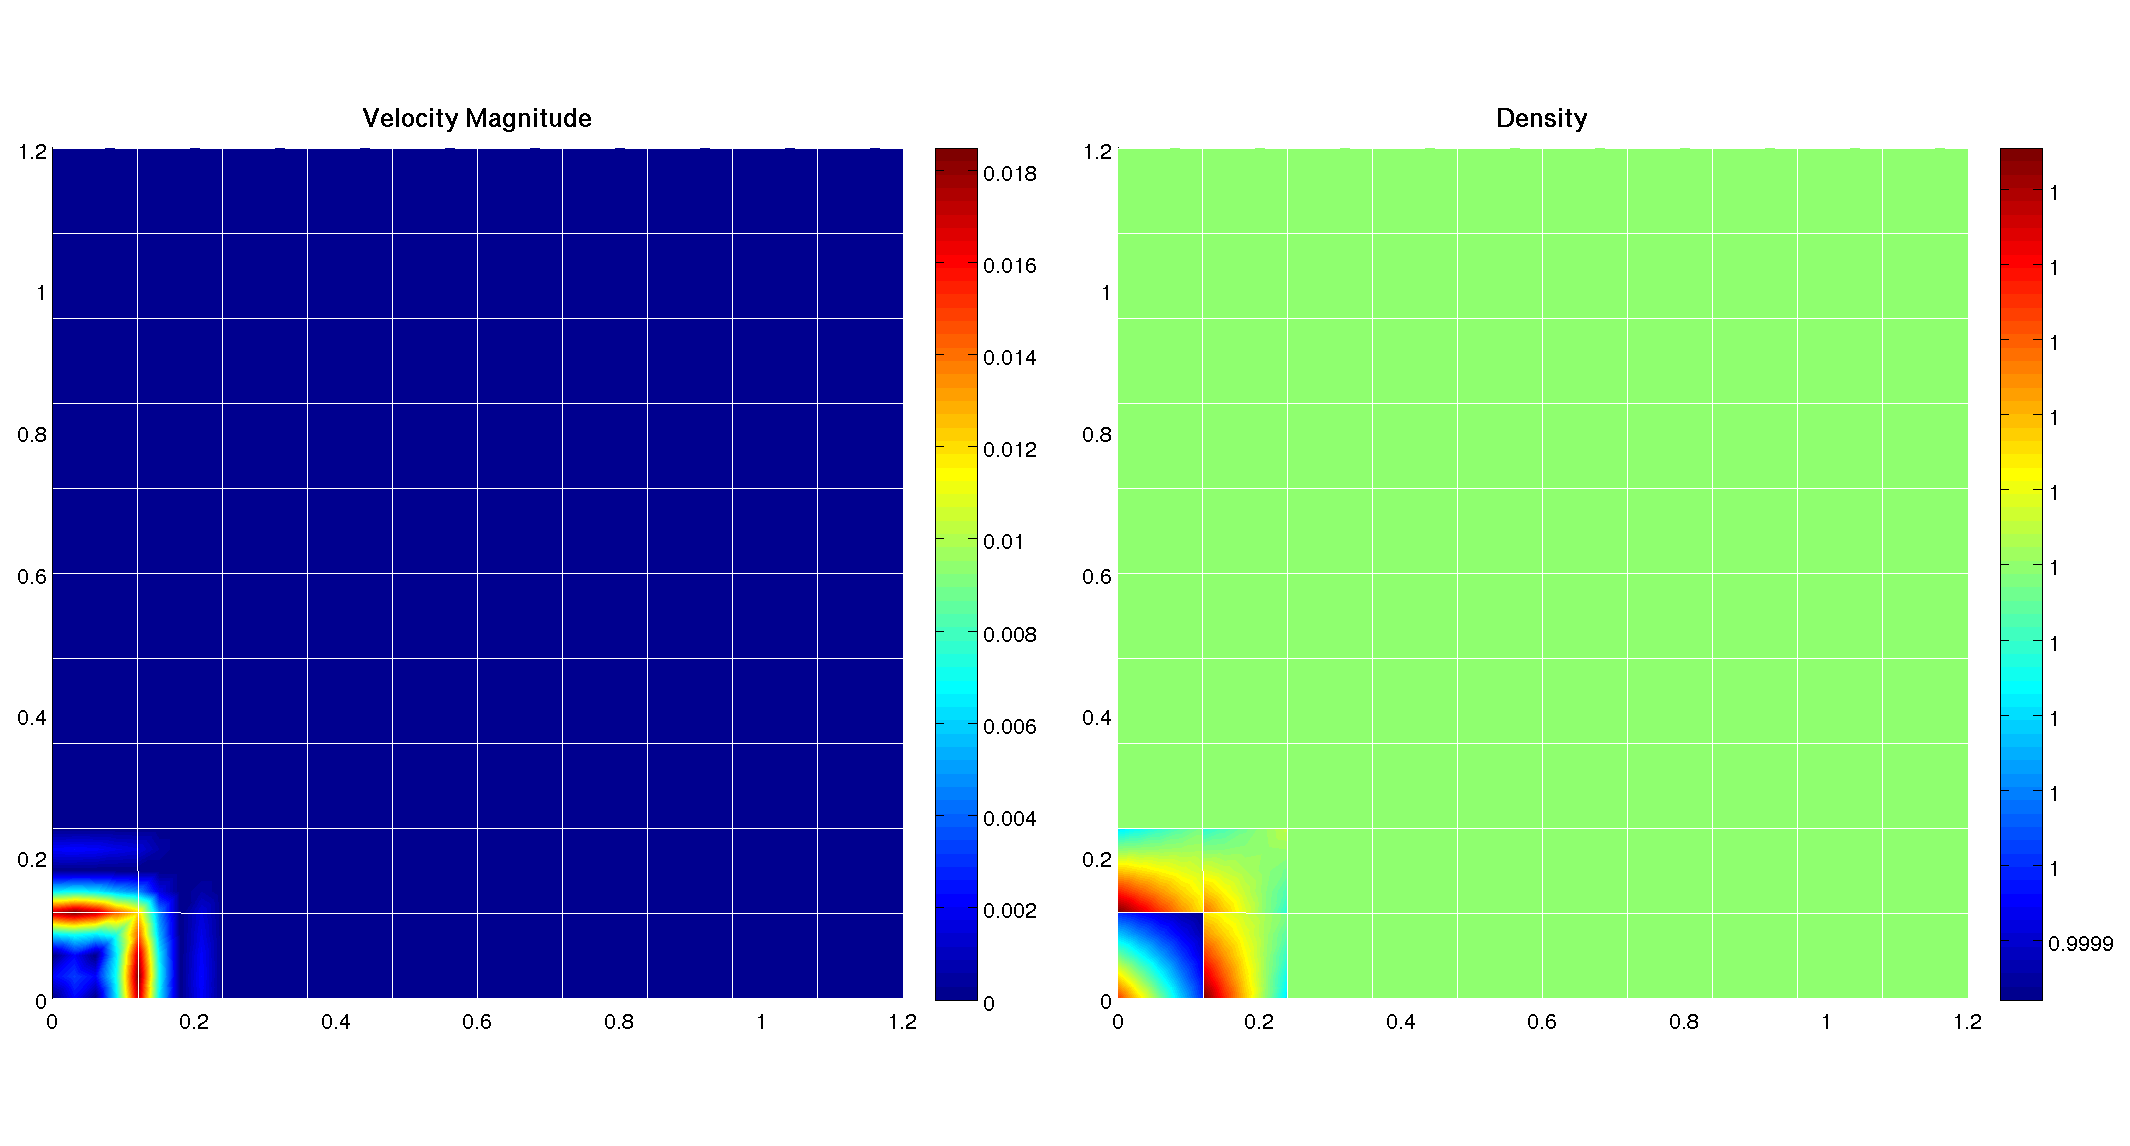
\includegraphics{./Images/SedovAnimation/SedovAnimation_00.png}
    \newframe[1]
    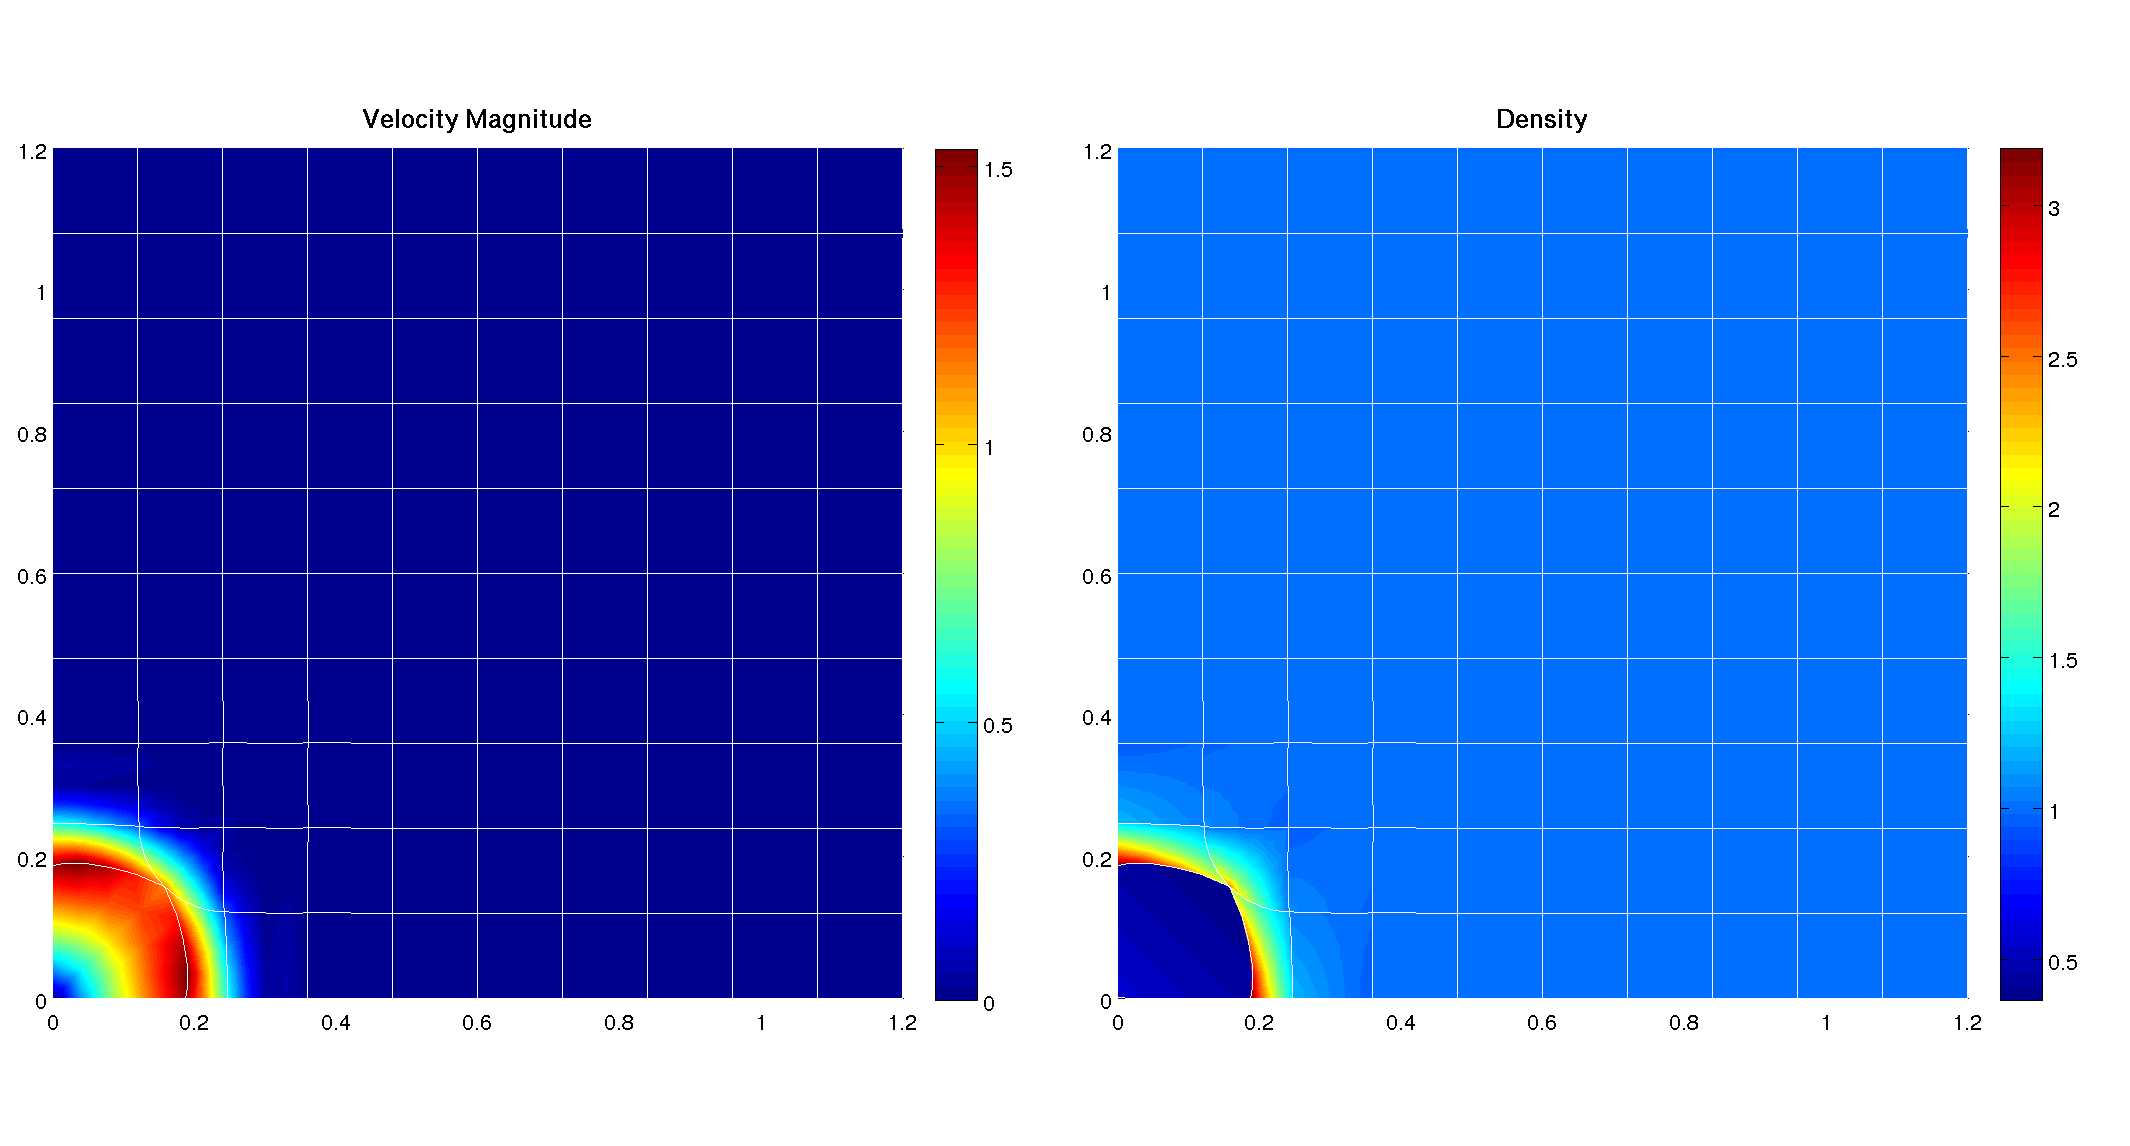
\includegraphics{./Images/SedovAnimation/SedovAnimation_10.png}
    \newframe[1]
    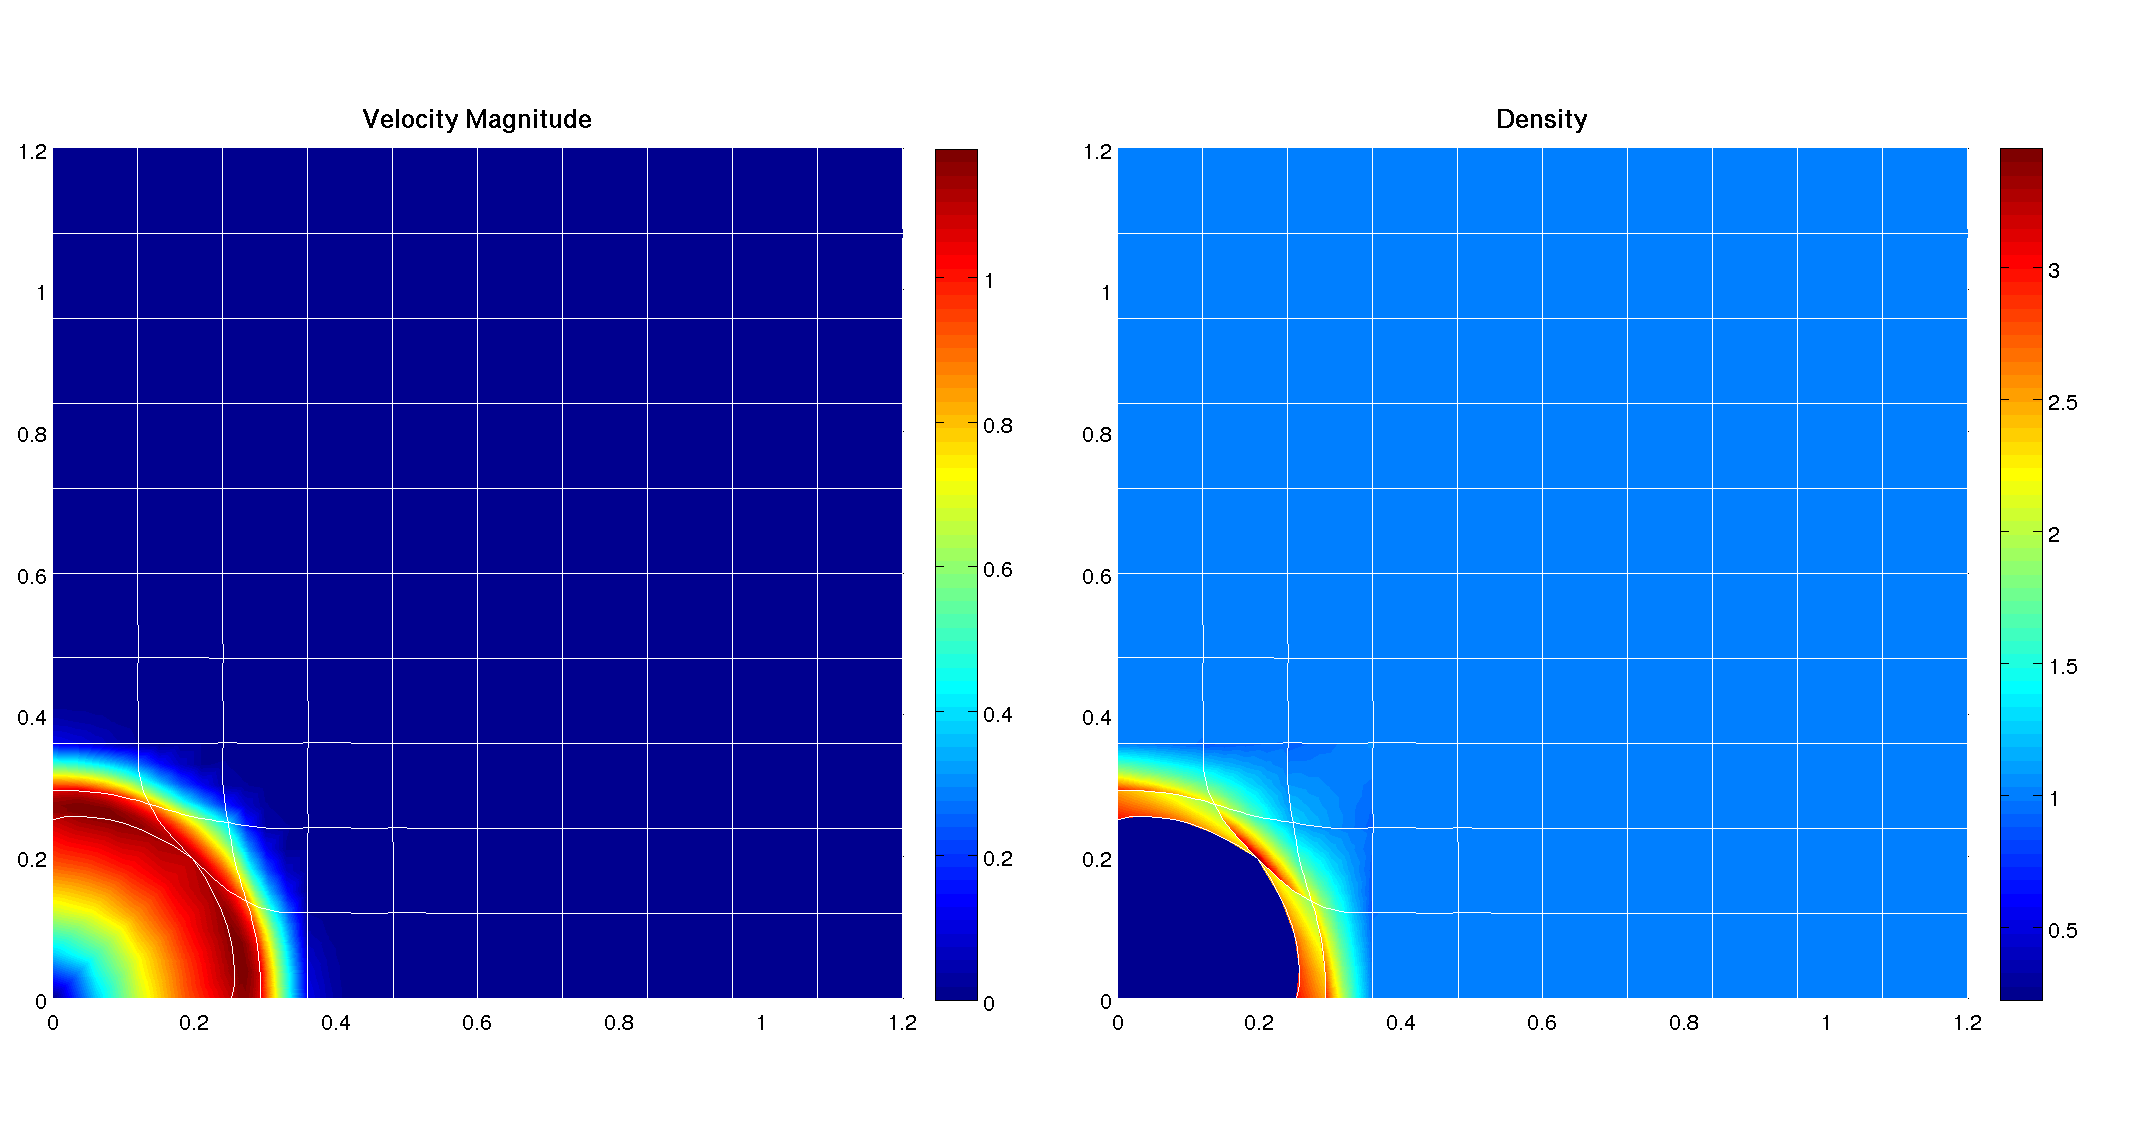
\includegraphics{./Images/SedovAnimation/SedovAnimation_20.png}
    \newframe[1]
    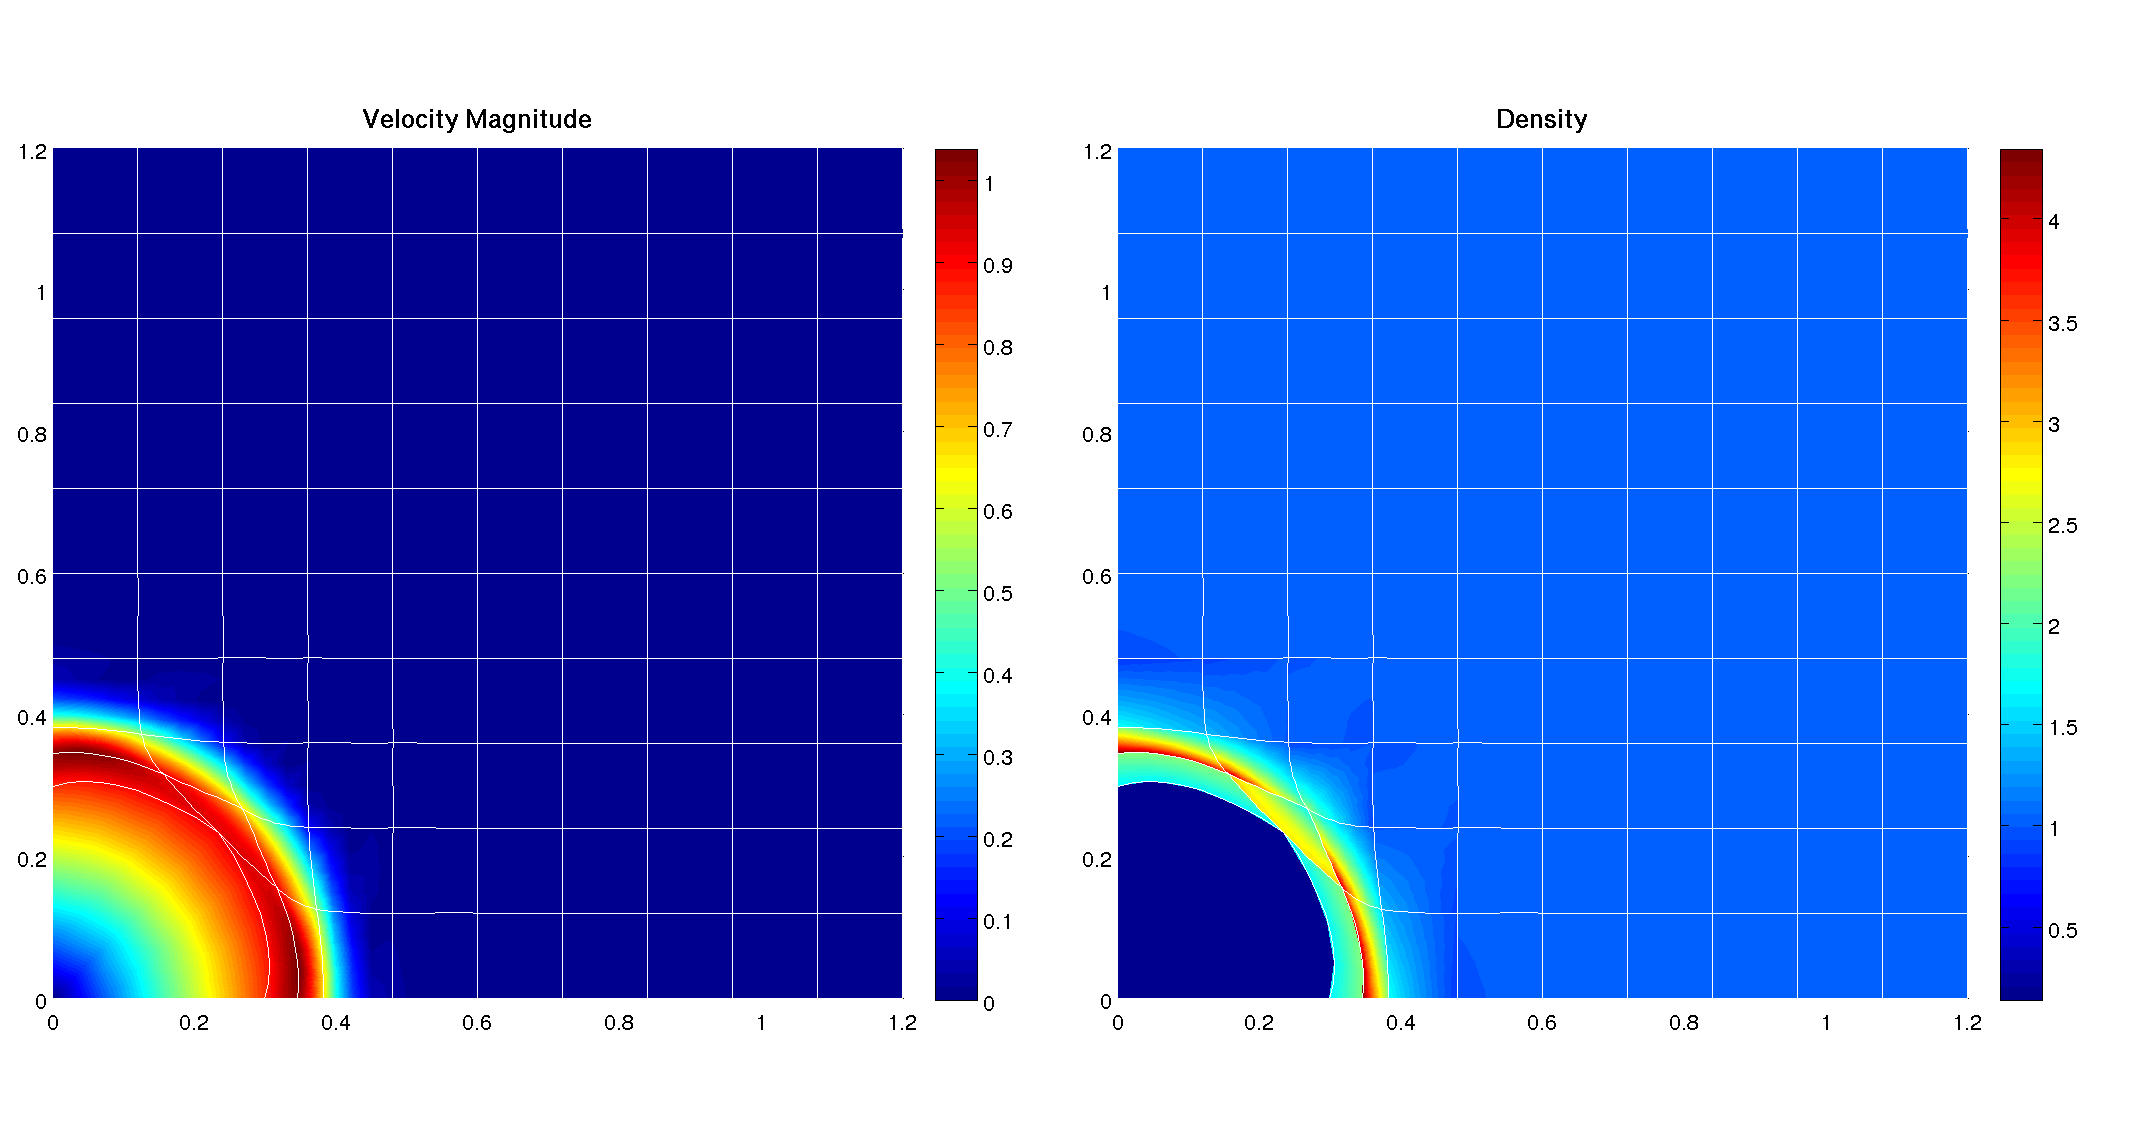
\includegraphics{./Images/SedovAnimation/SedovAnimation_30.png}
    \newframe[1]
    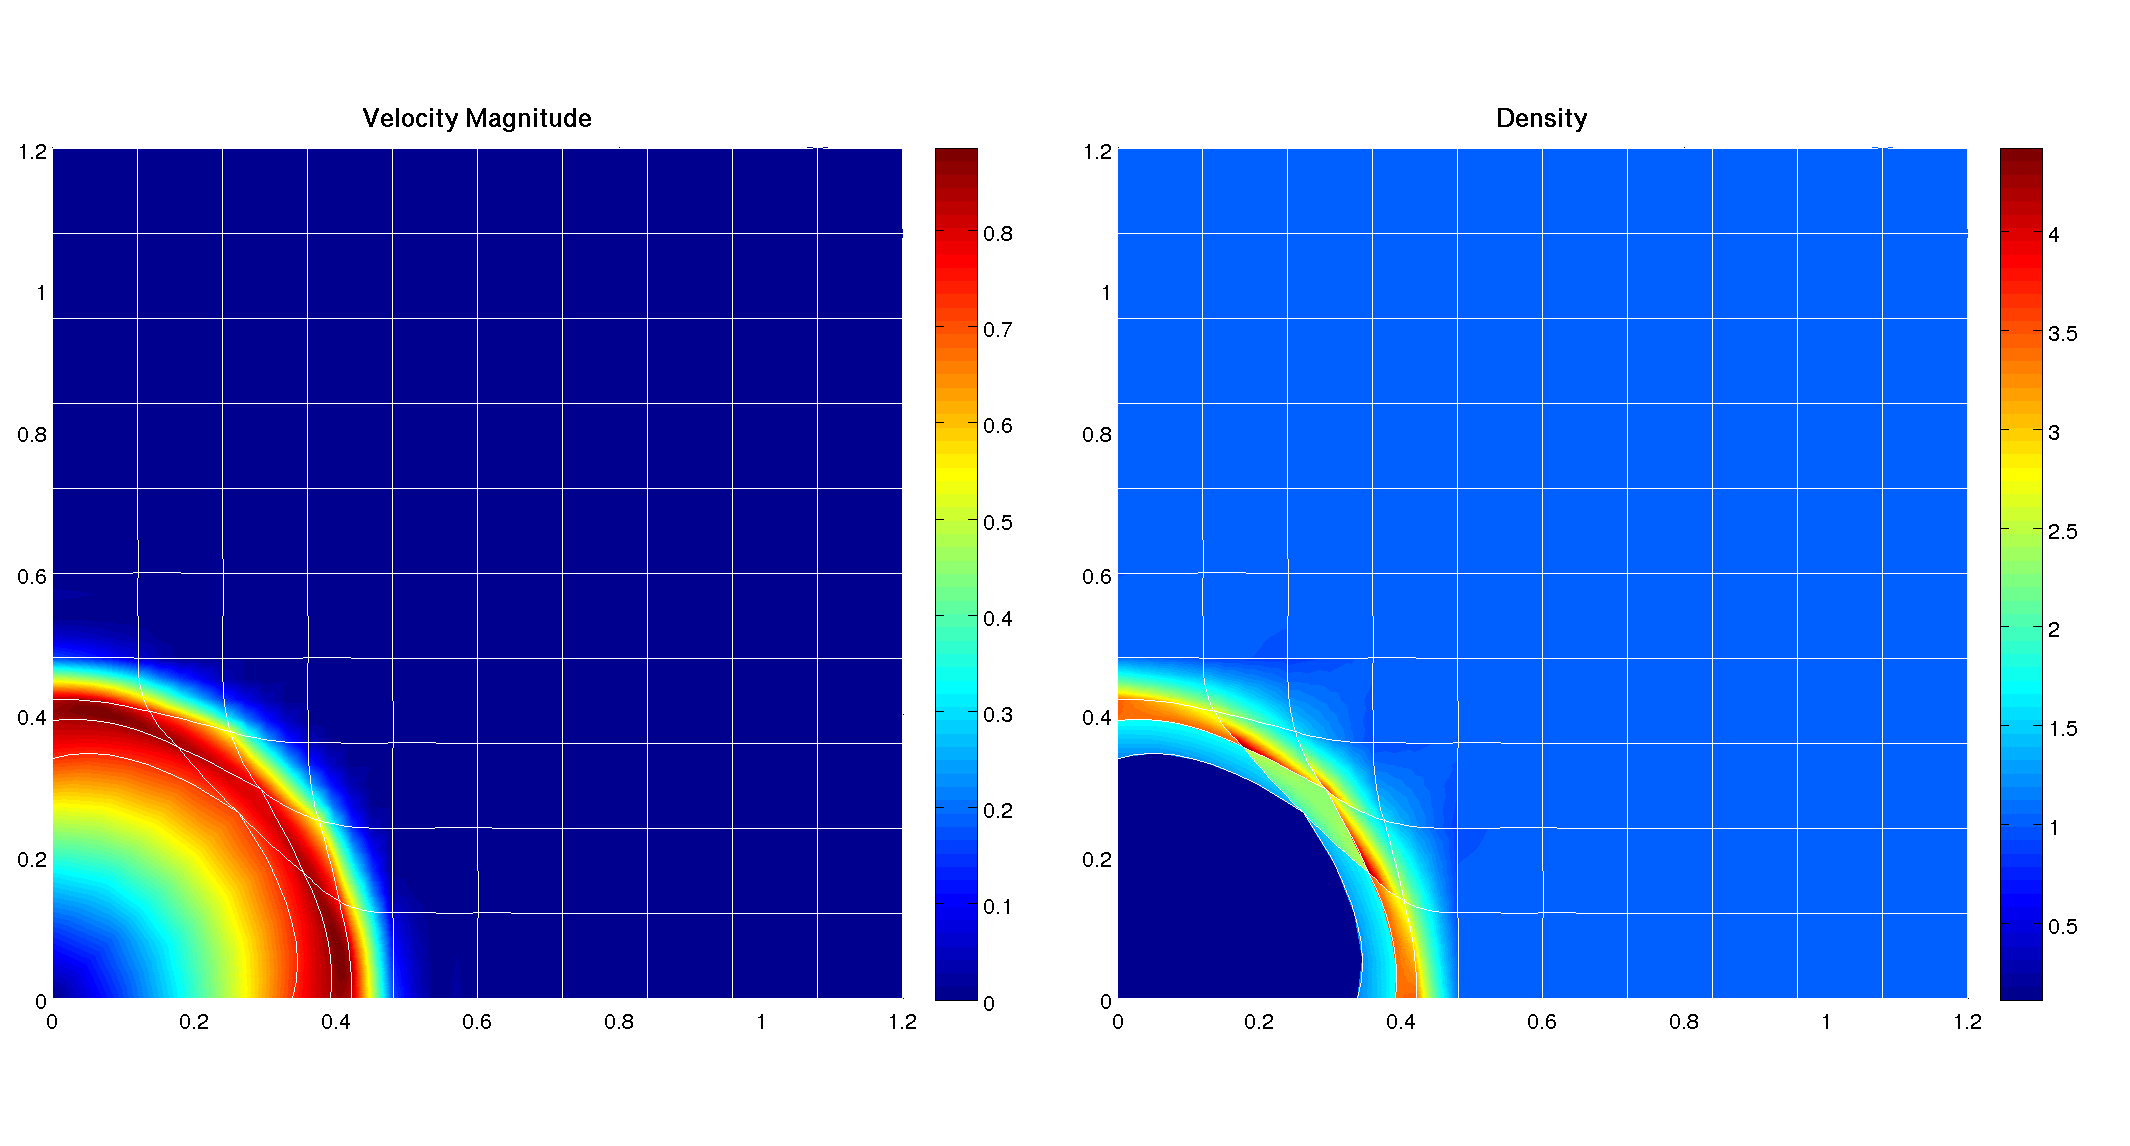
\includegraphics{./Images/SedovAnimation/SedovAnimation_40.png}
    \newframe[1]
    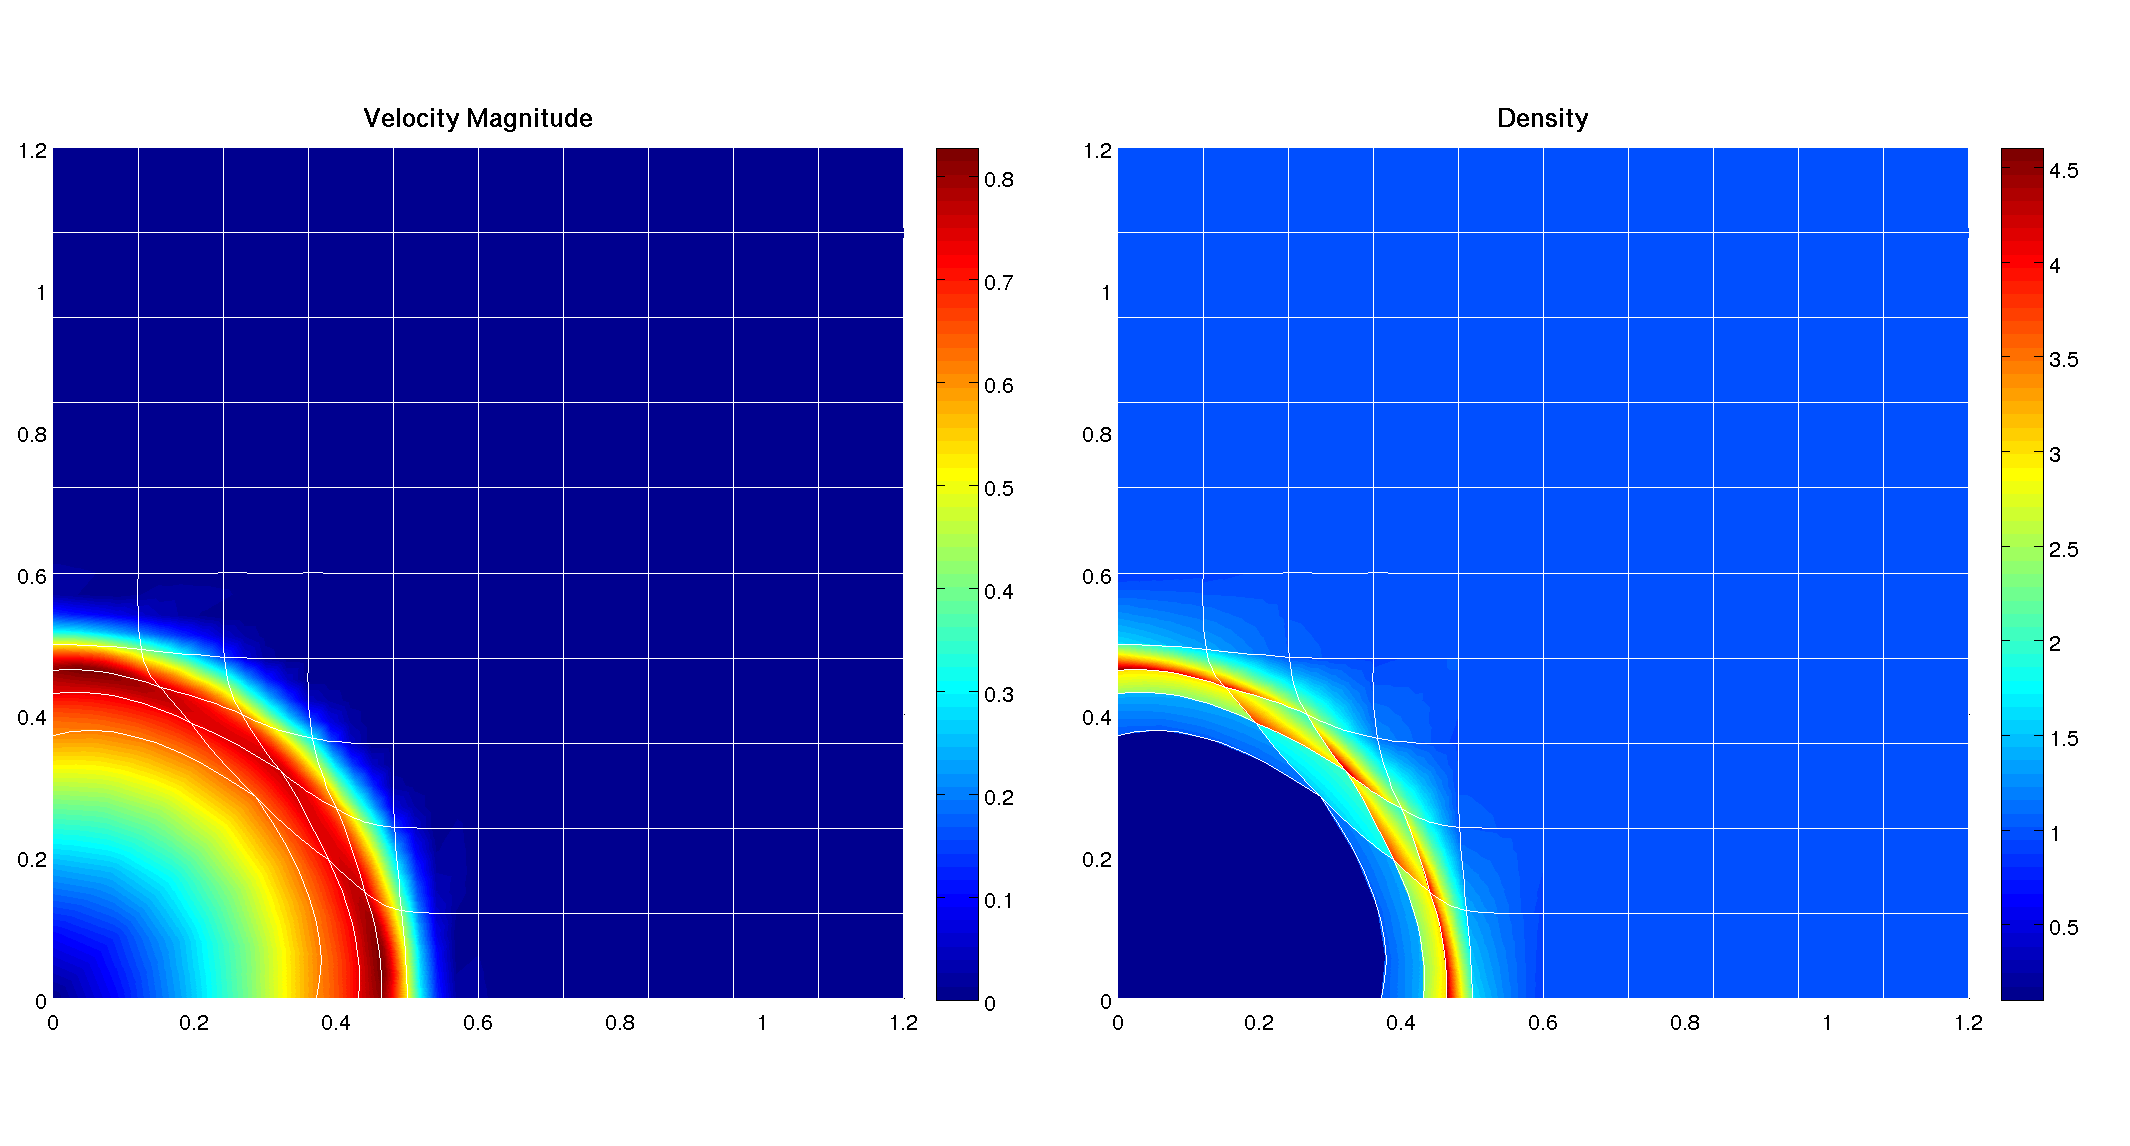
\includegraphics{./Images/SedovAnimation/SedovAnimation_50.png}
    \newframe[1]
    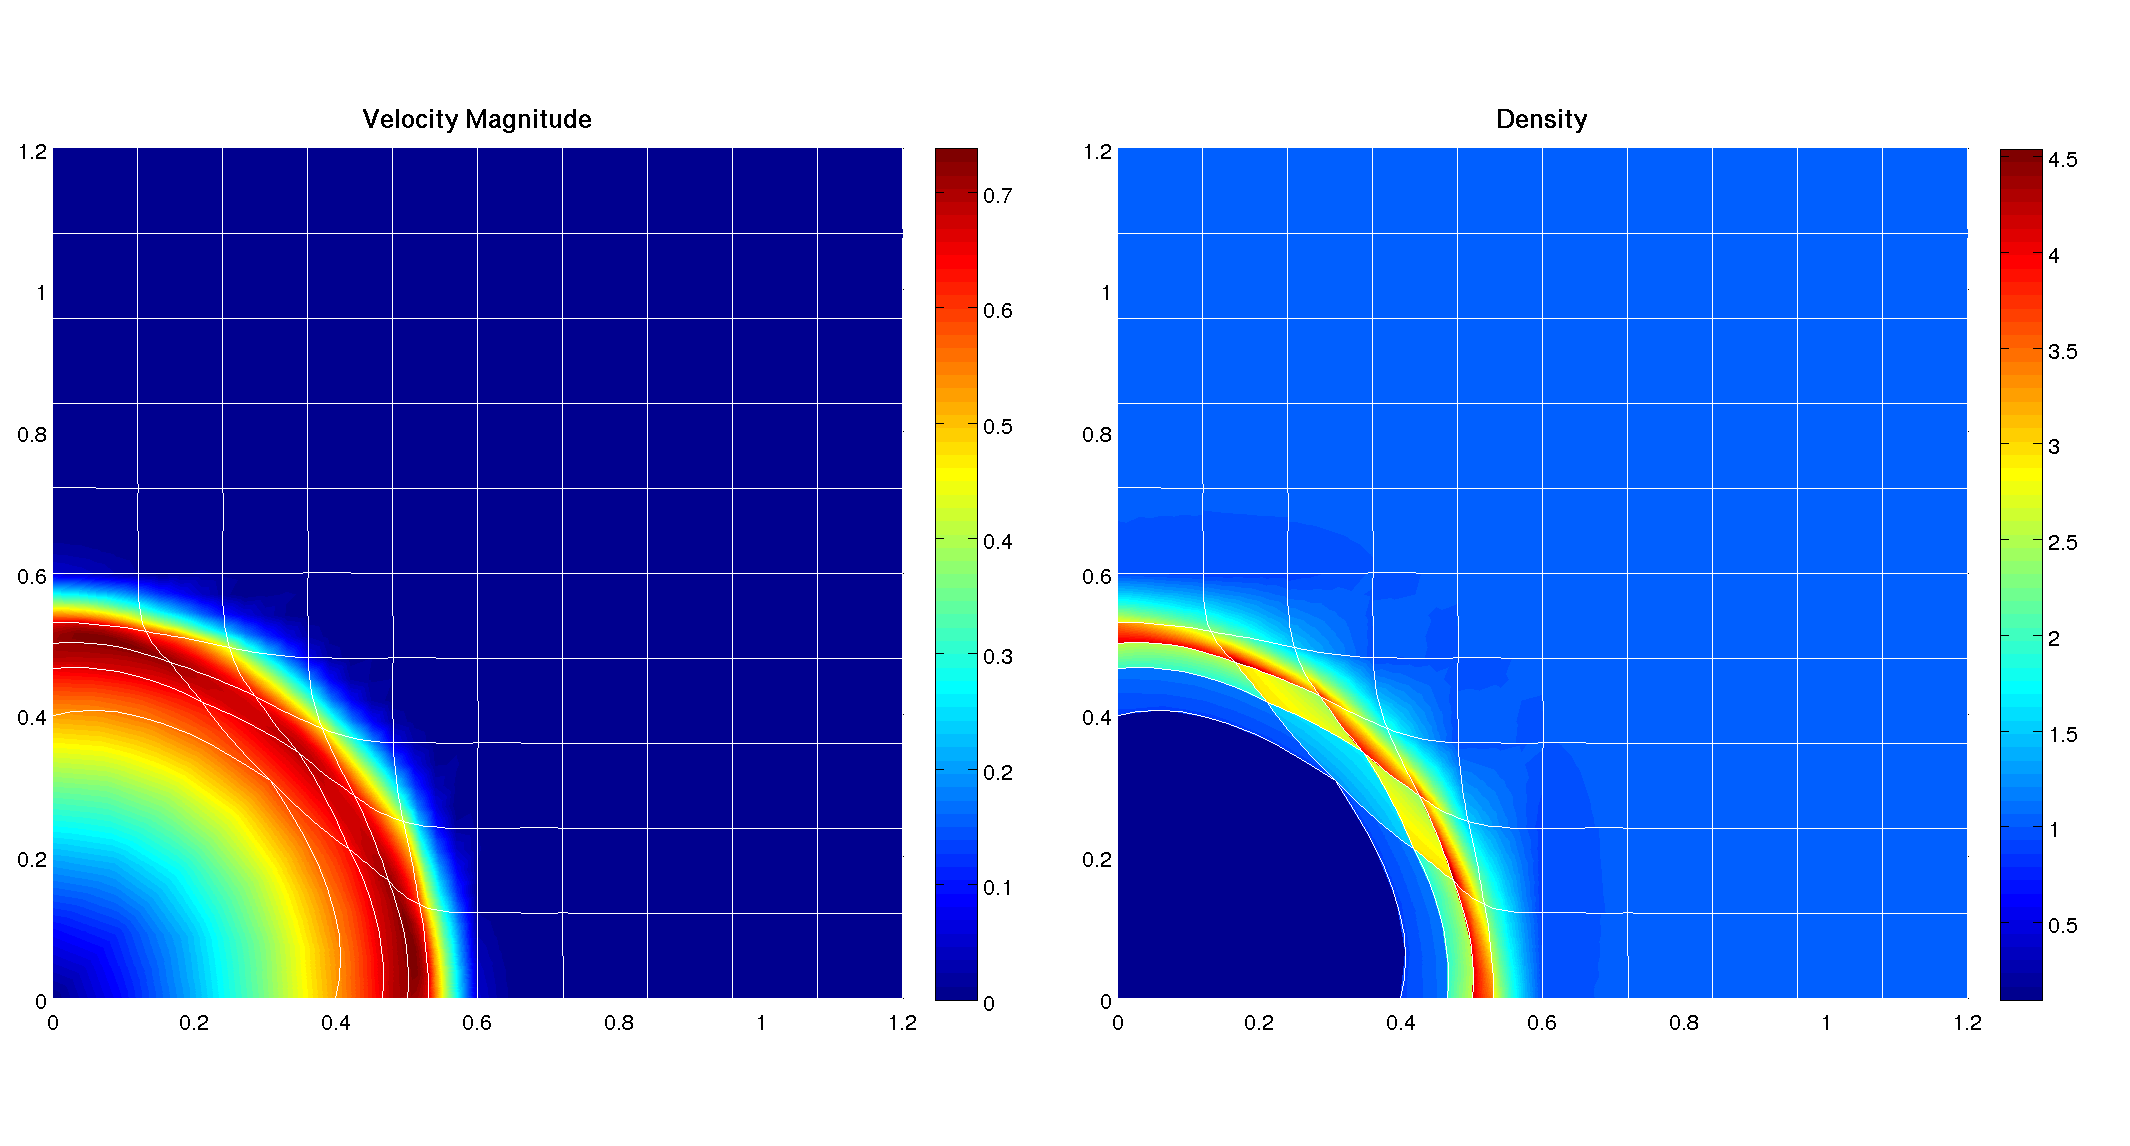
\includegraphics{./Images/SedovAnimation/SedovAnimation_60.png}
    \newframe[1]
    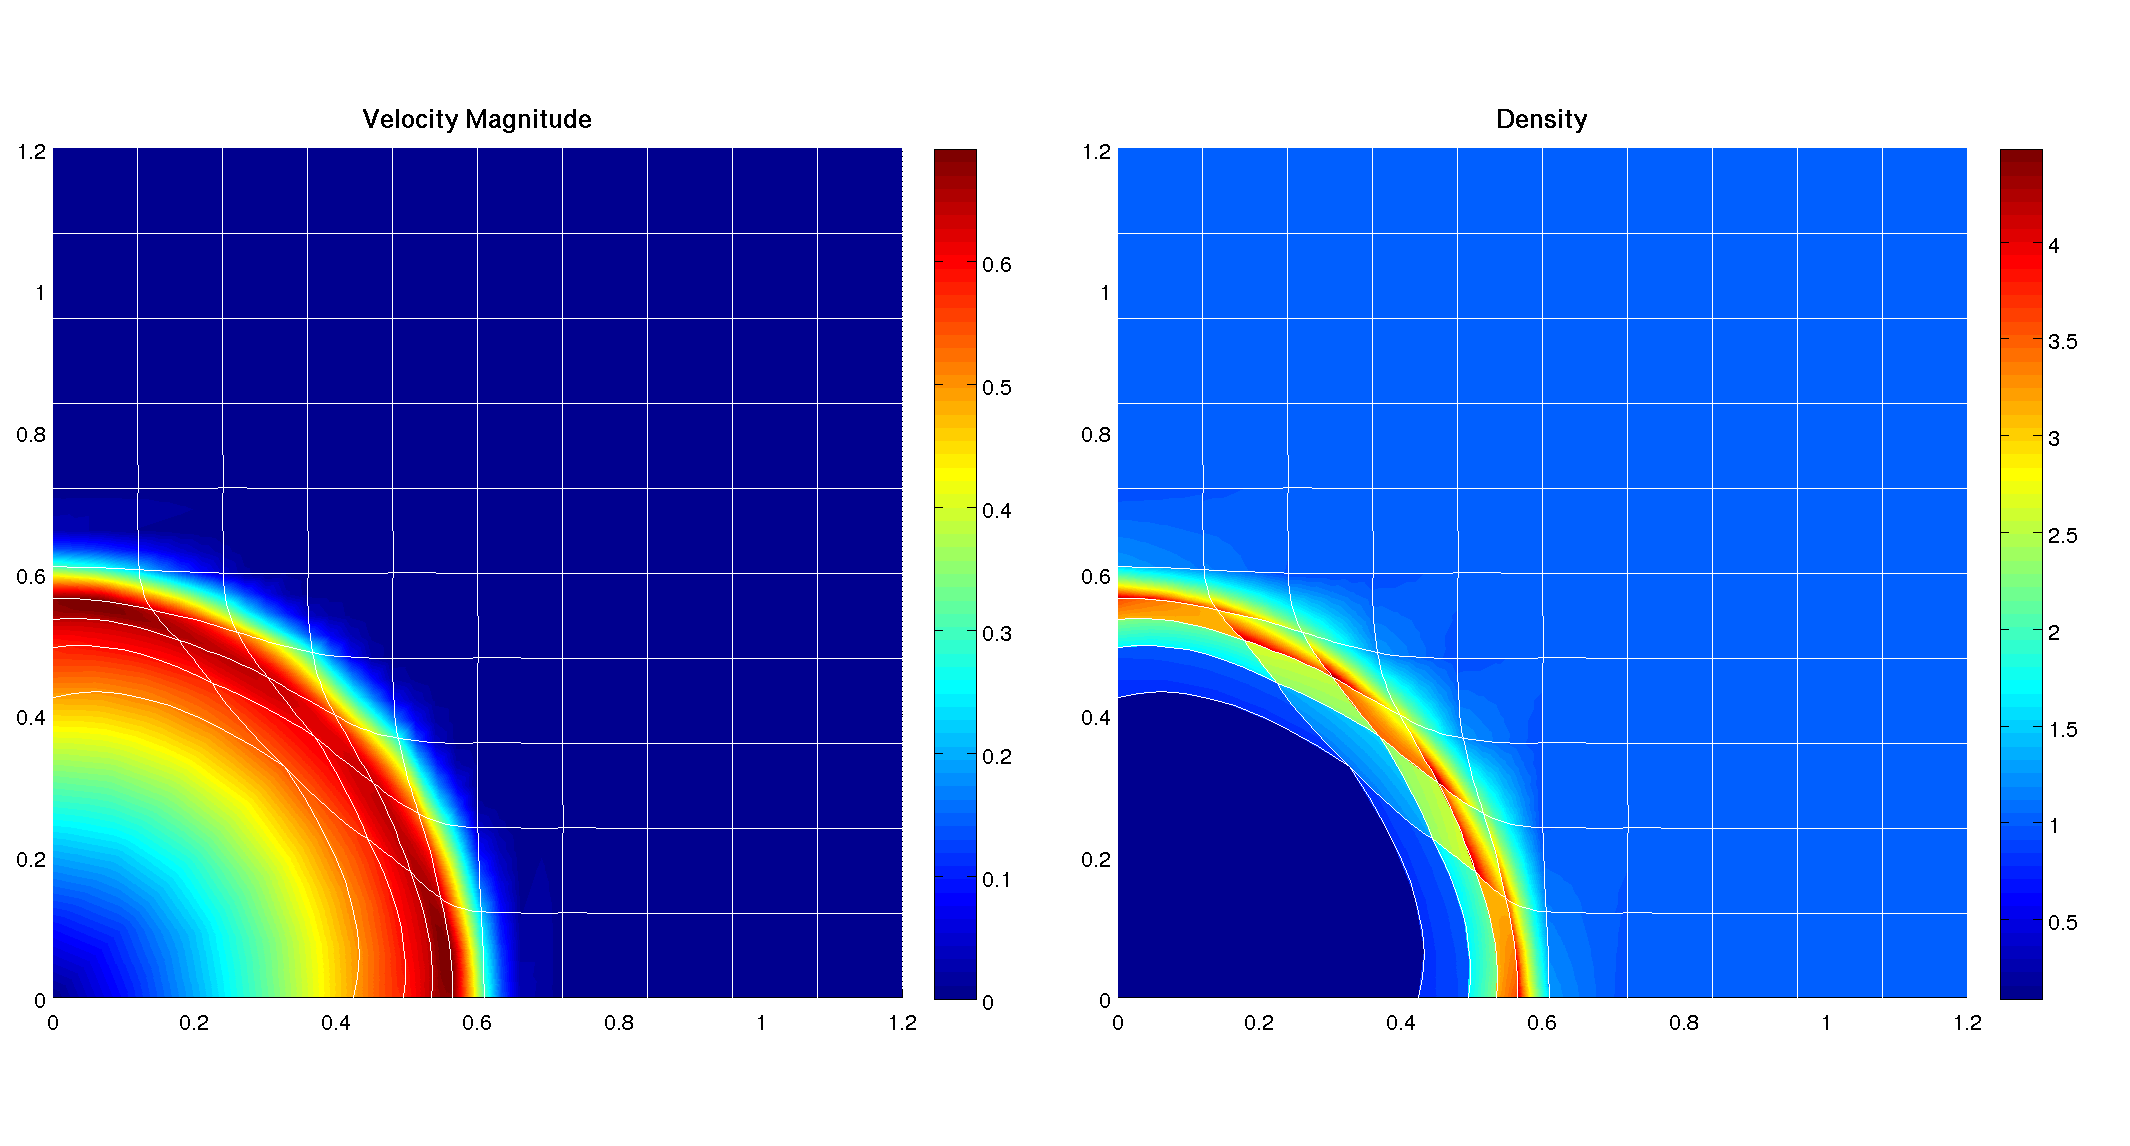
\includegraphics{./Images/SedovAnimation/SedovAnimation_70.png}
    \newframe[1]
    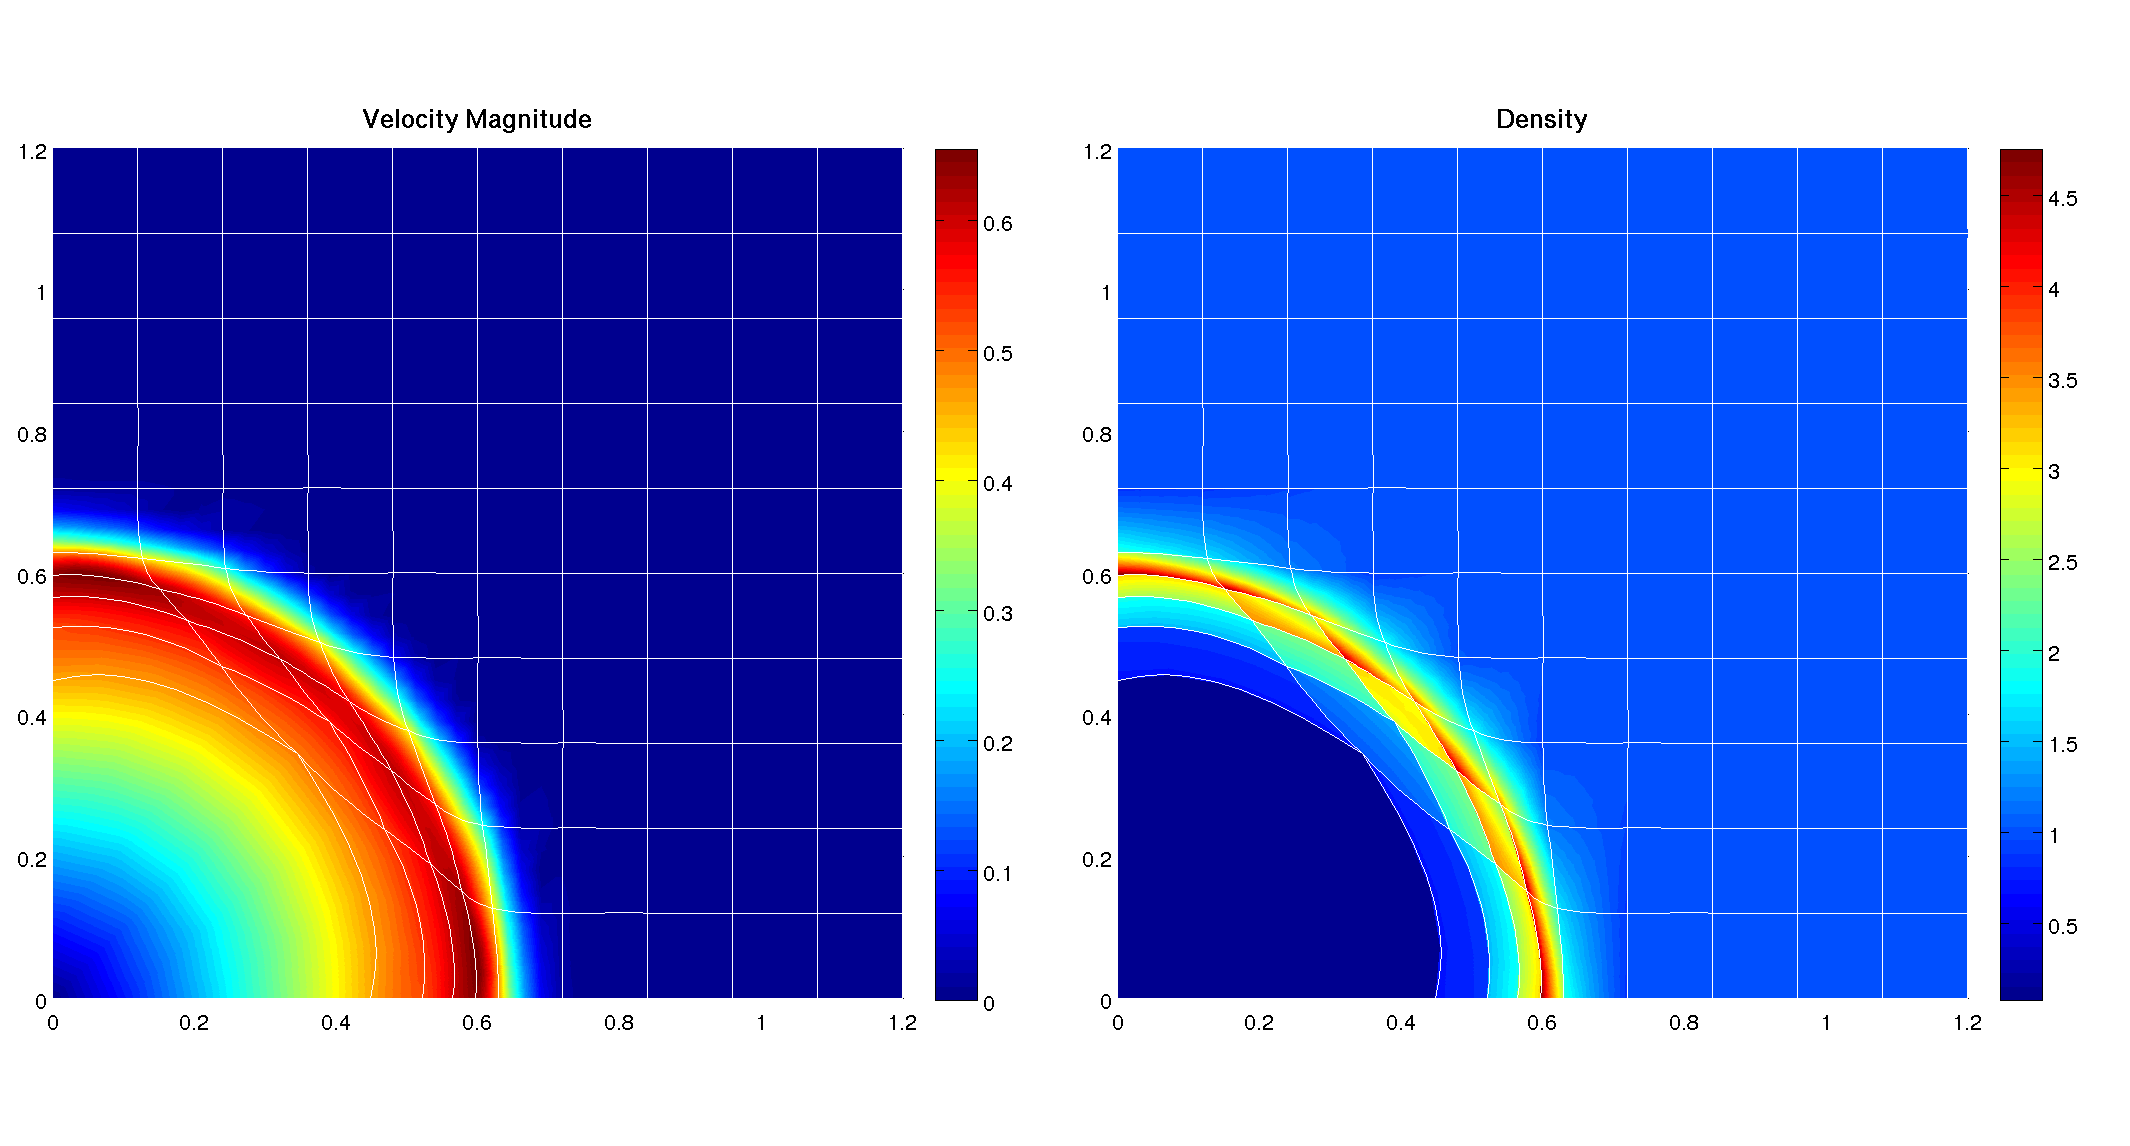
\includegraphics{./Images/SedovAnimation/SedovAnimation_80.png}
    \newframe[1]
    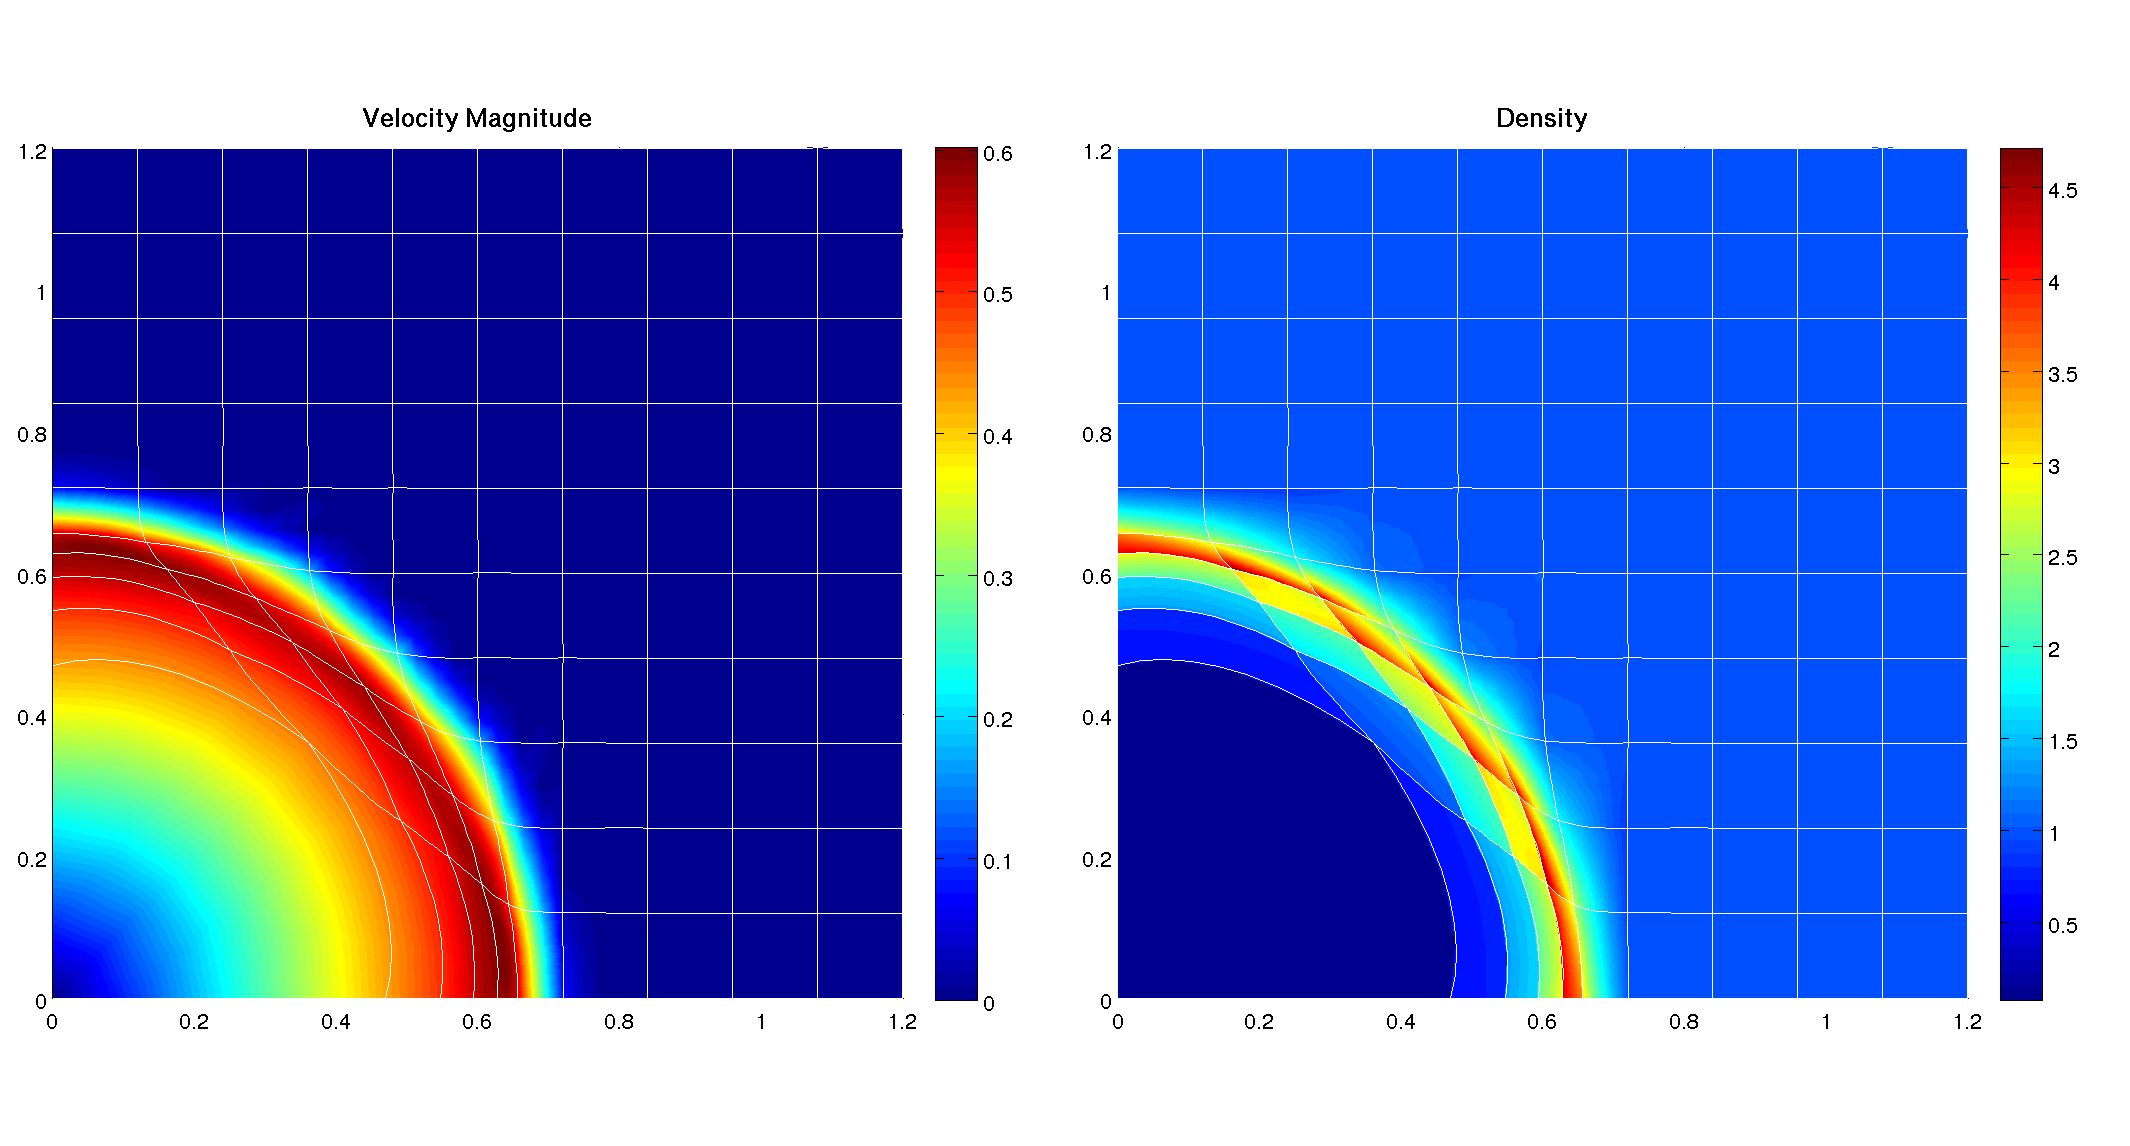
\includegraphics{./Images/SedovAnimation/SedovAnimation_90.png}
    \newframe[1]
    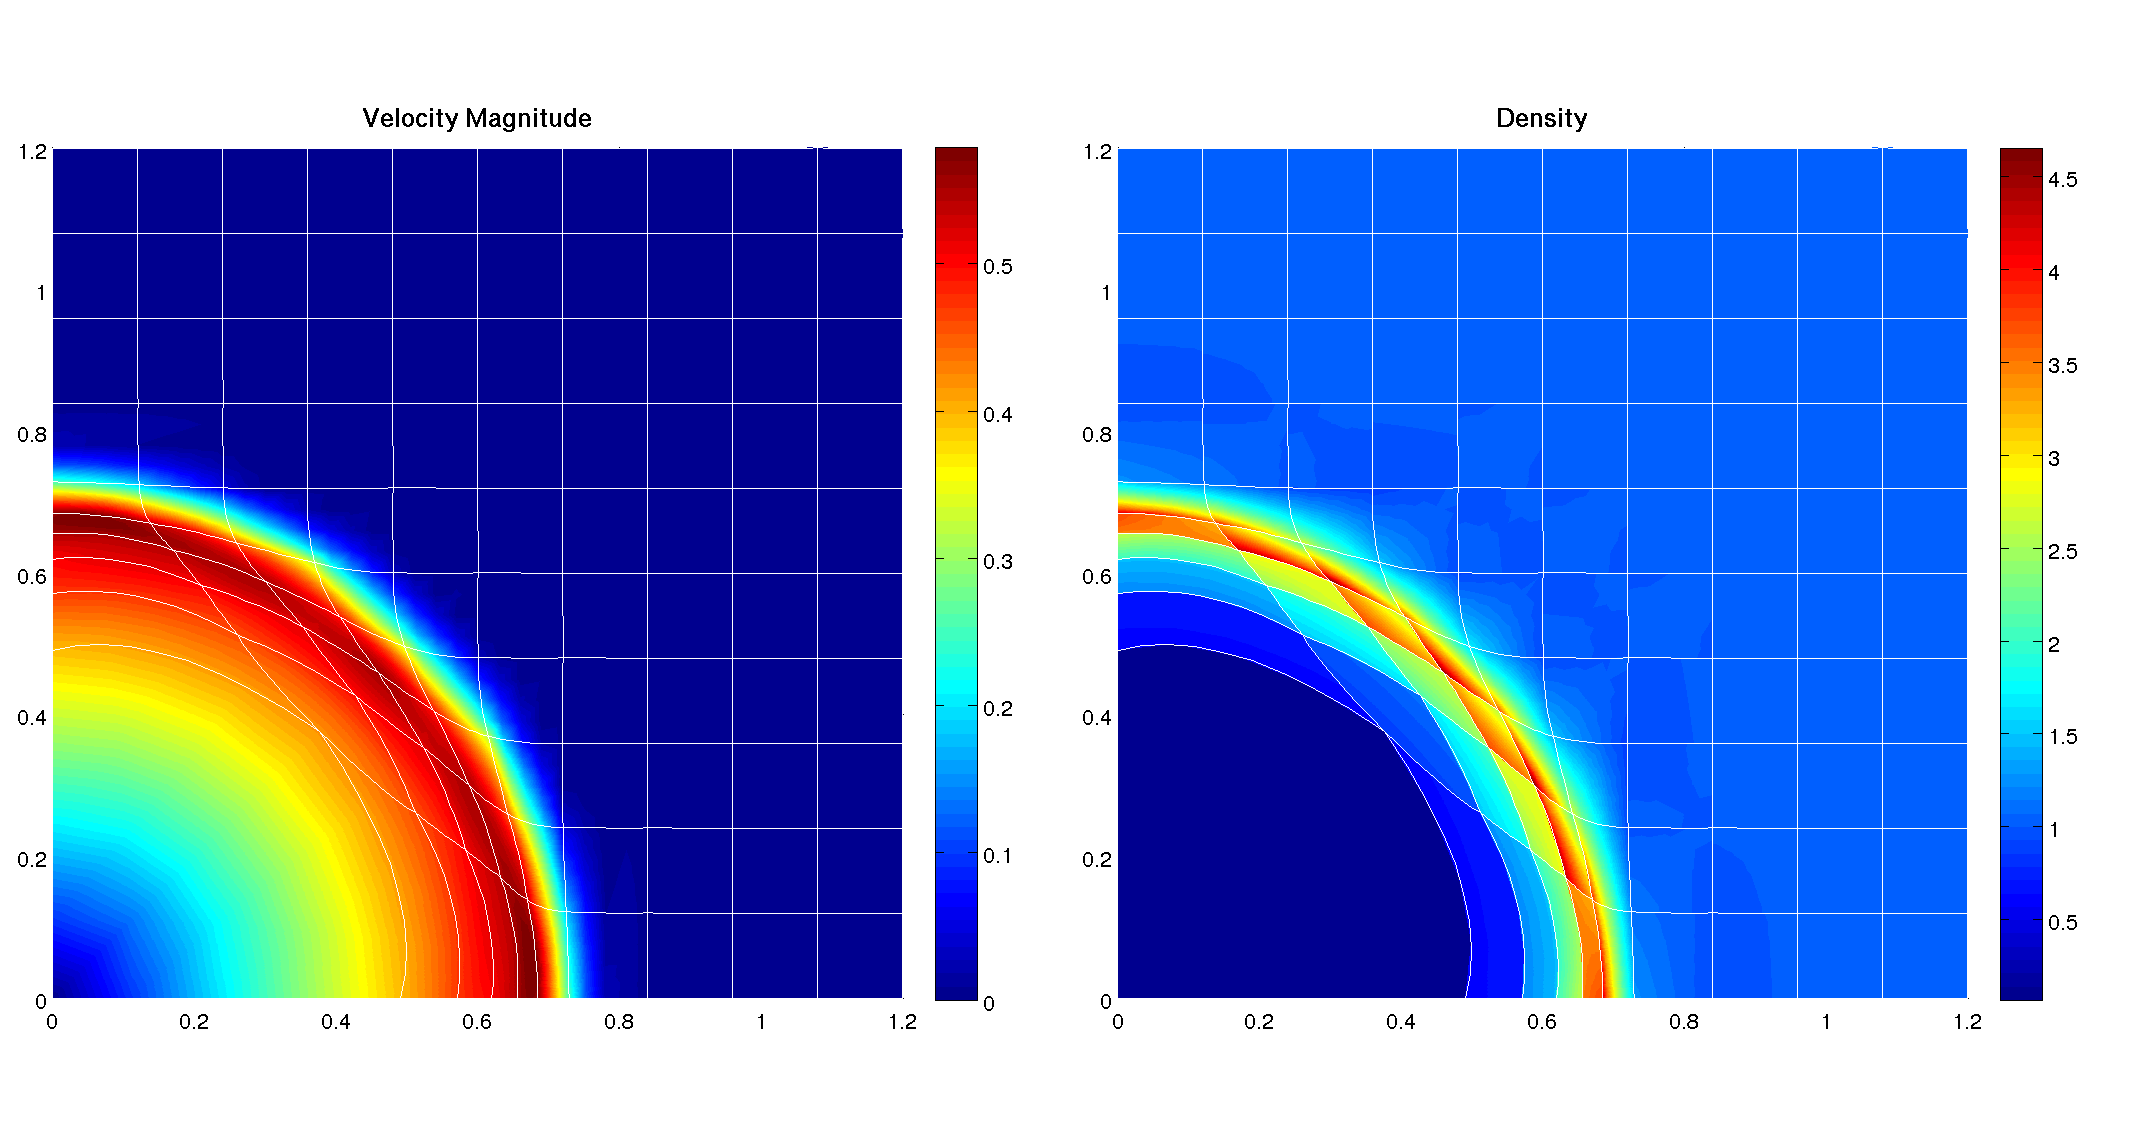
\includegraphics{./Images/SedovAnimation/SedovAnimation_100.png}
    \newframe[1]
    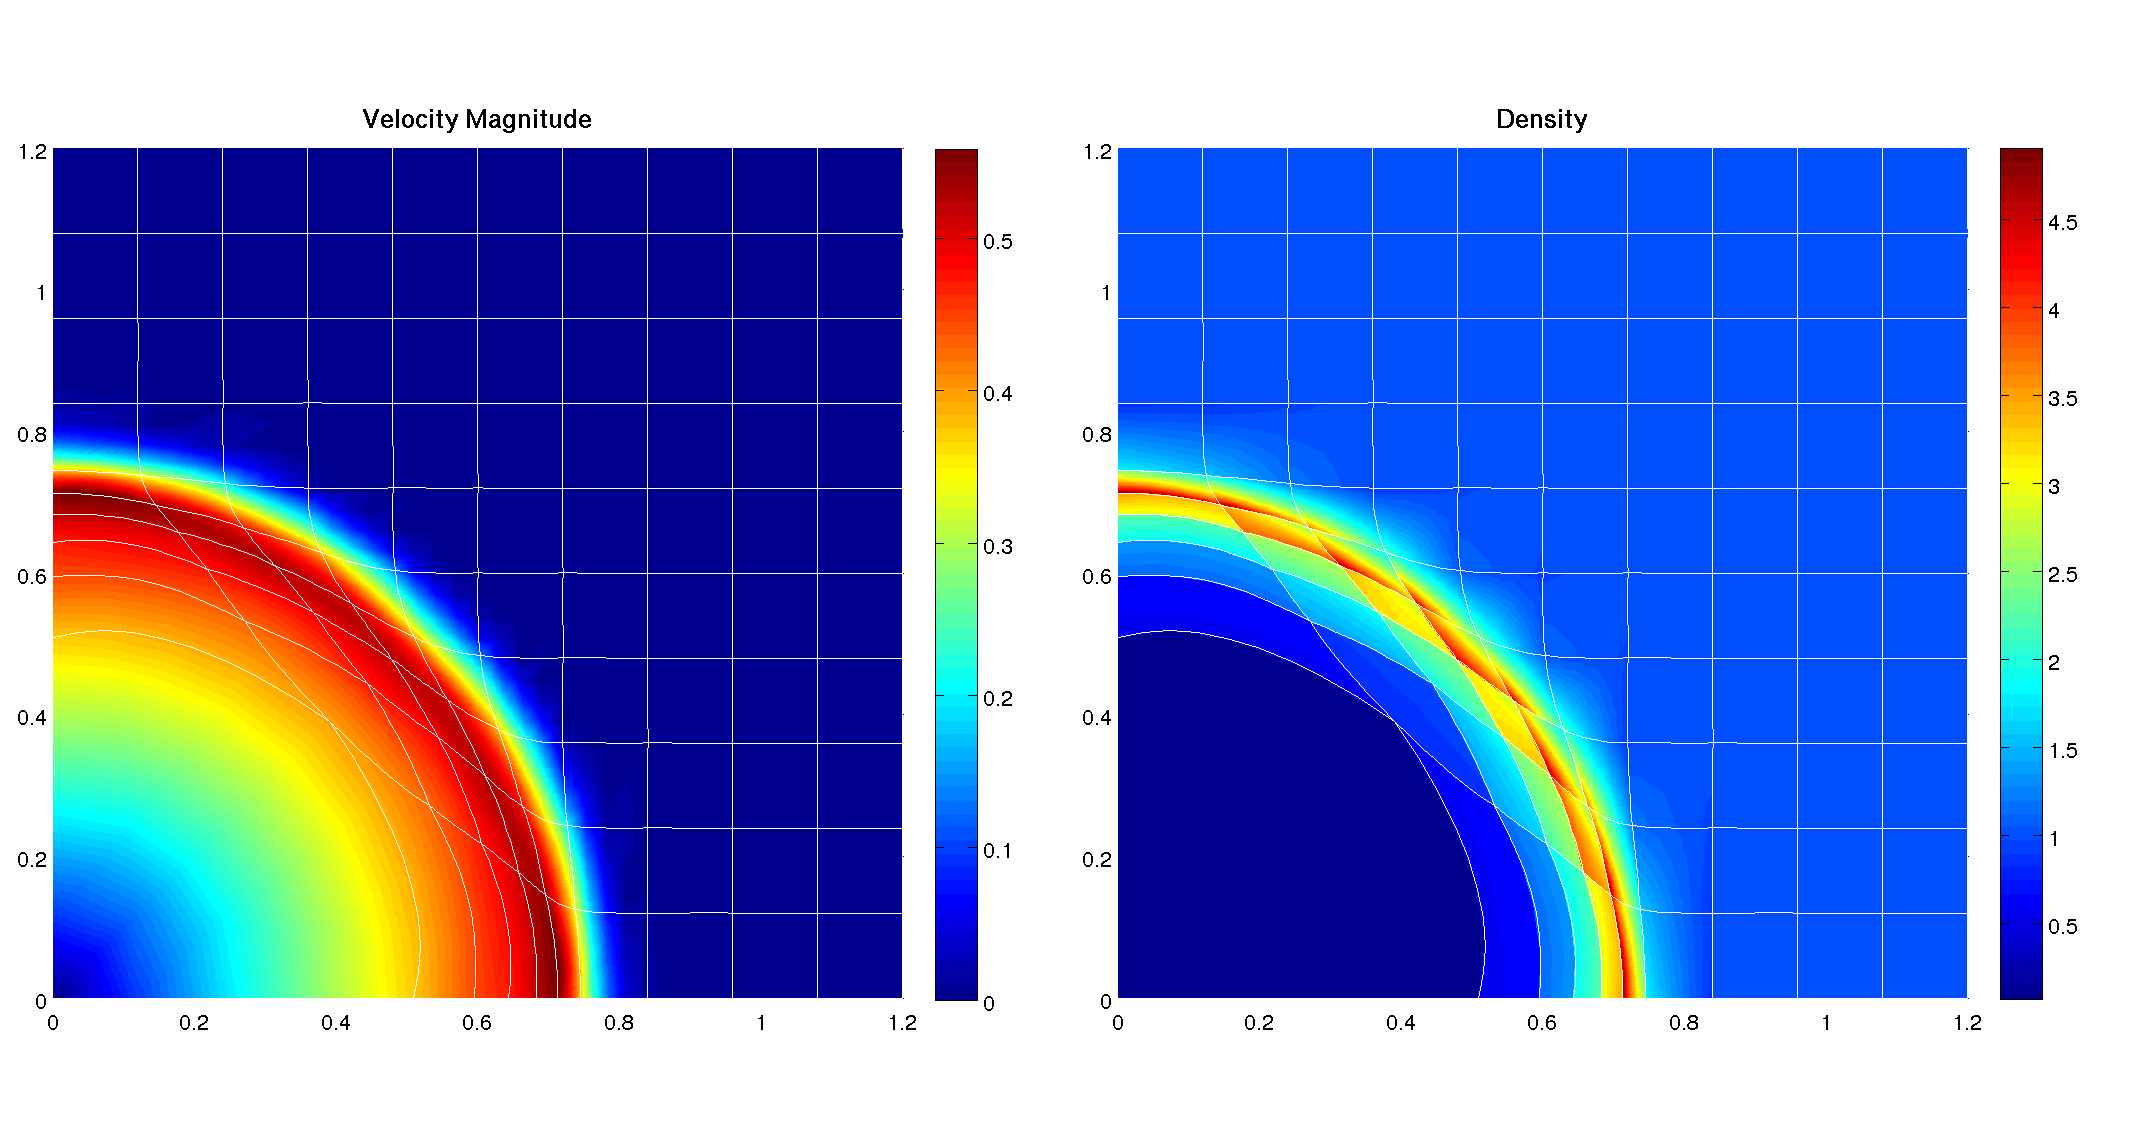
\includegraphics{./Images/SedovAnimation/SedovAnimation_110.png}
    \newframe[1]
    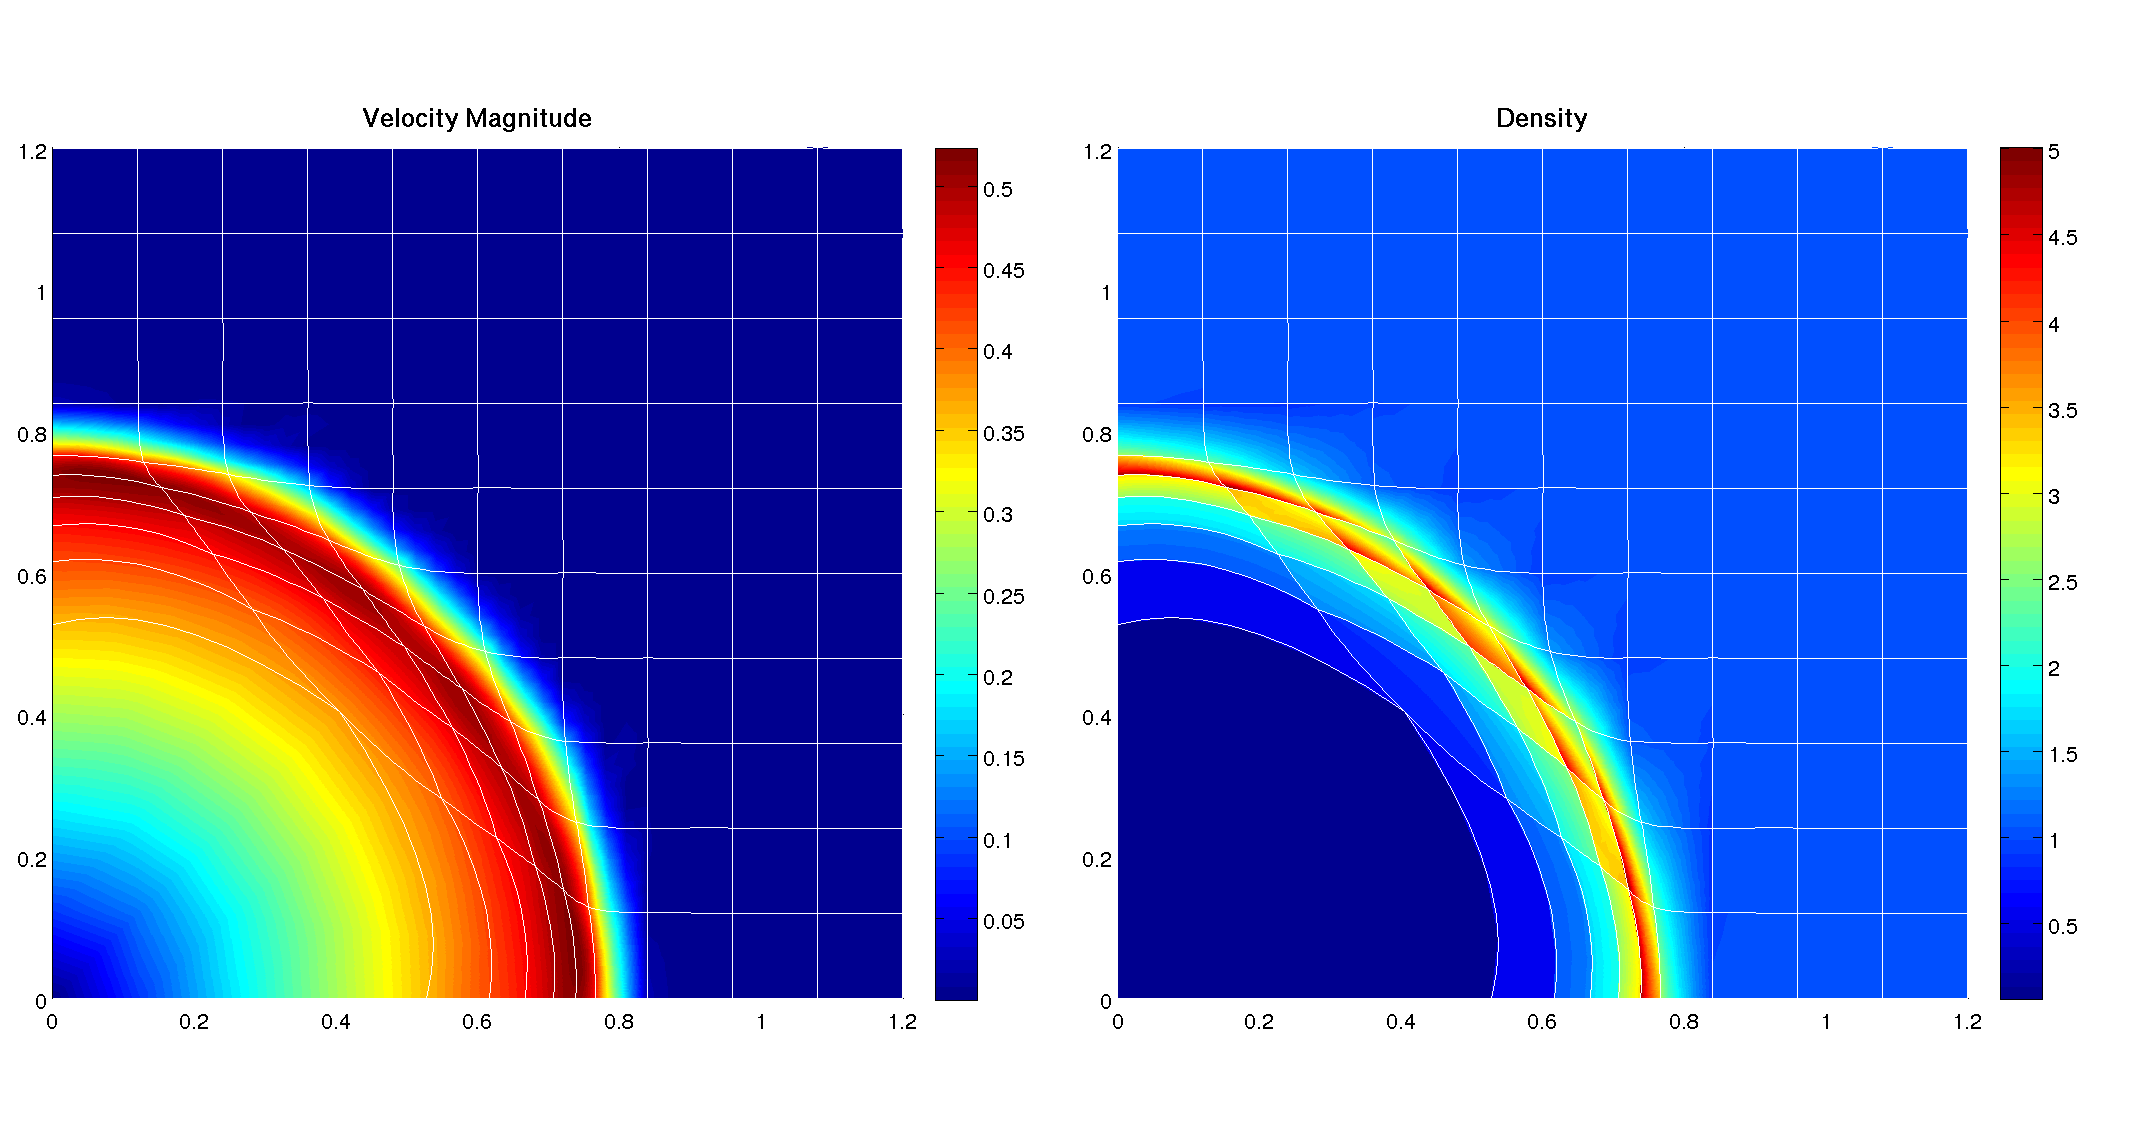
\includegraphics{./Images/SedovAnimation/SedovAnimation_120.png}
    \newframe[1]
    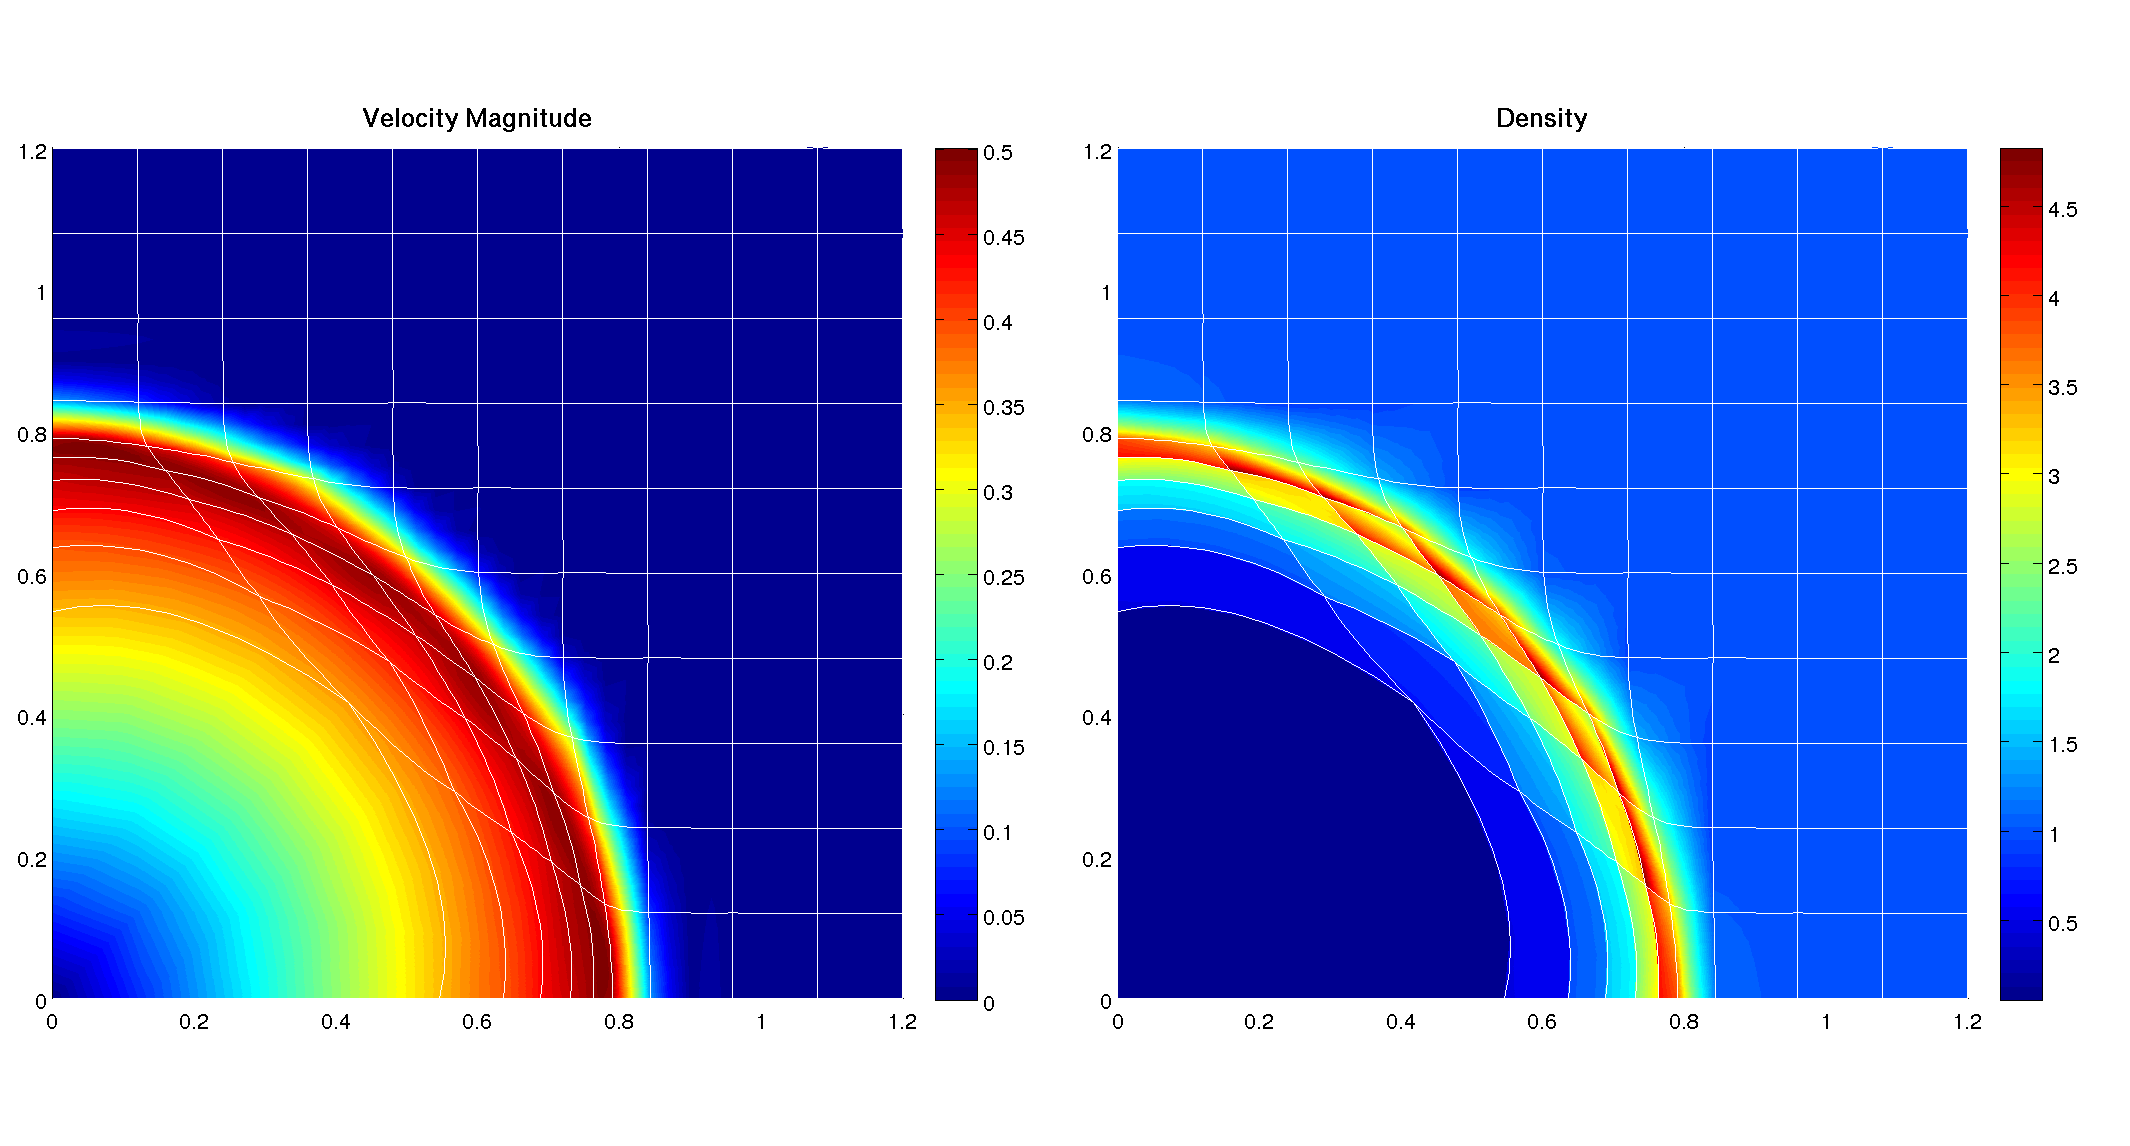
\includegraphics{./Images/SedovAnimation/SedovAnimation_130.png}
    \newframe[1]
    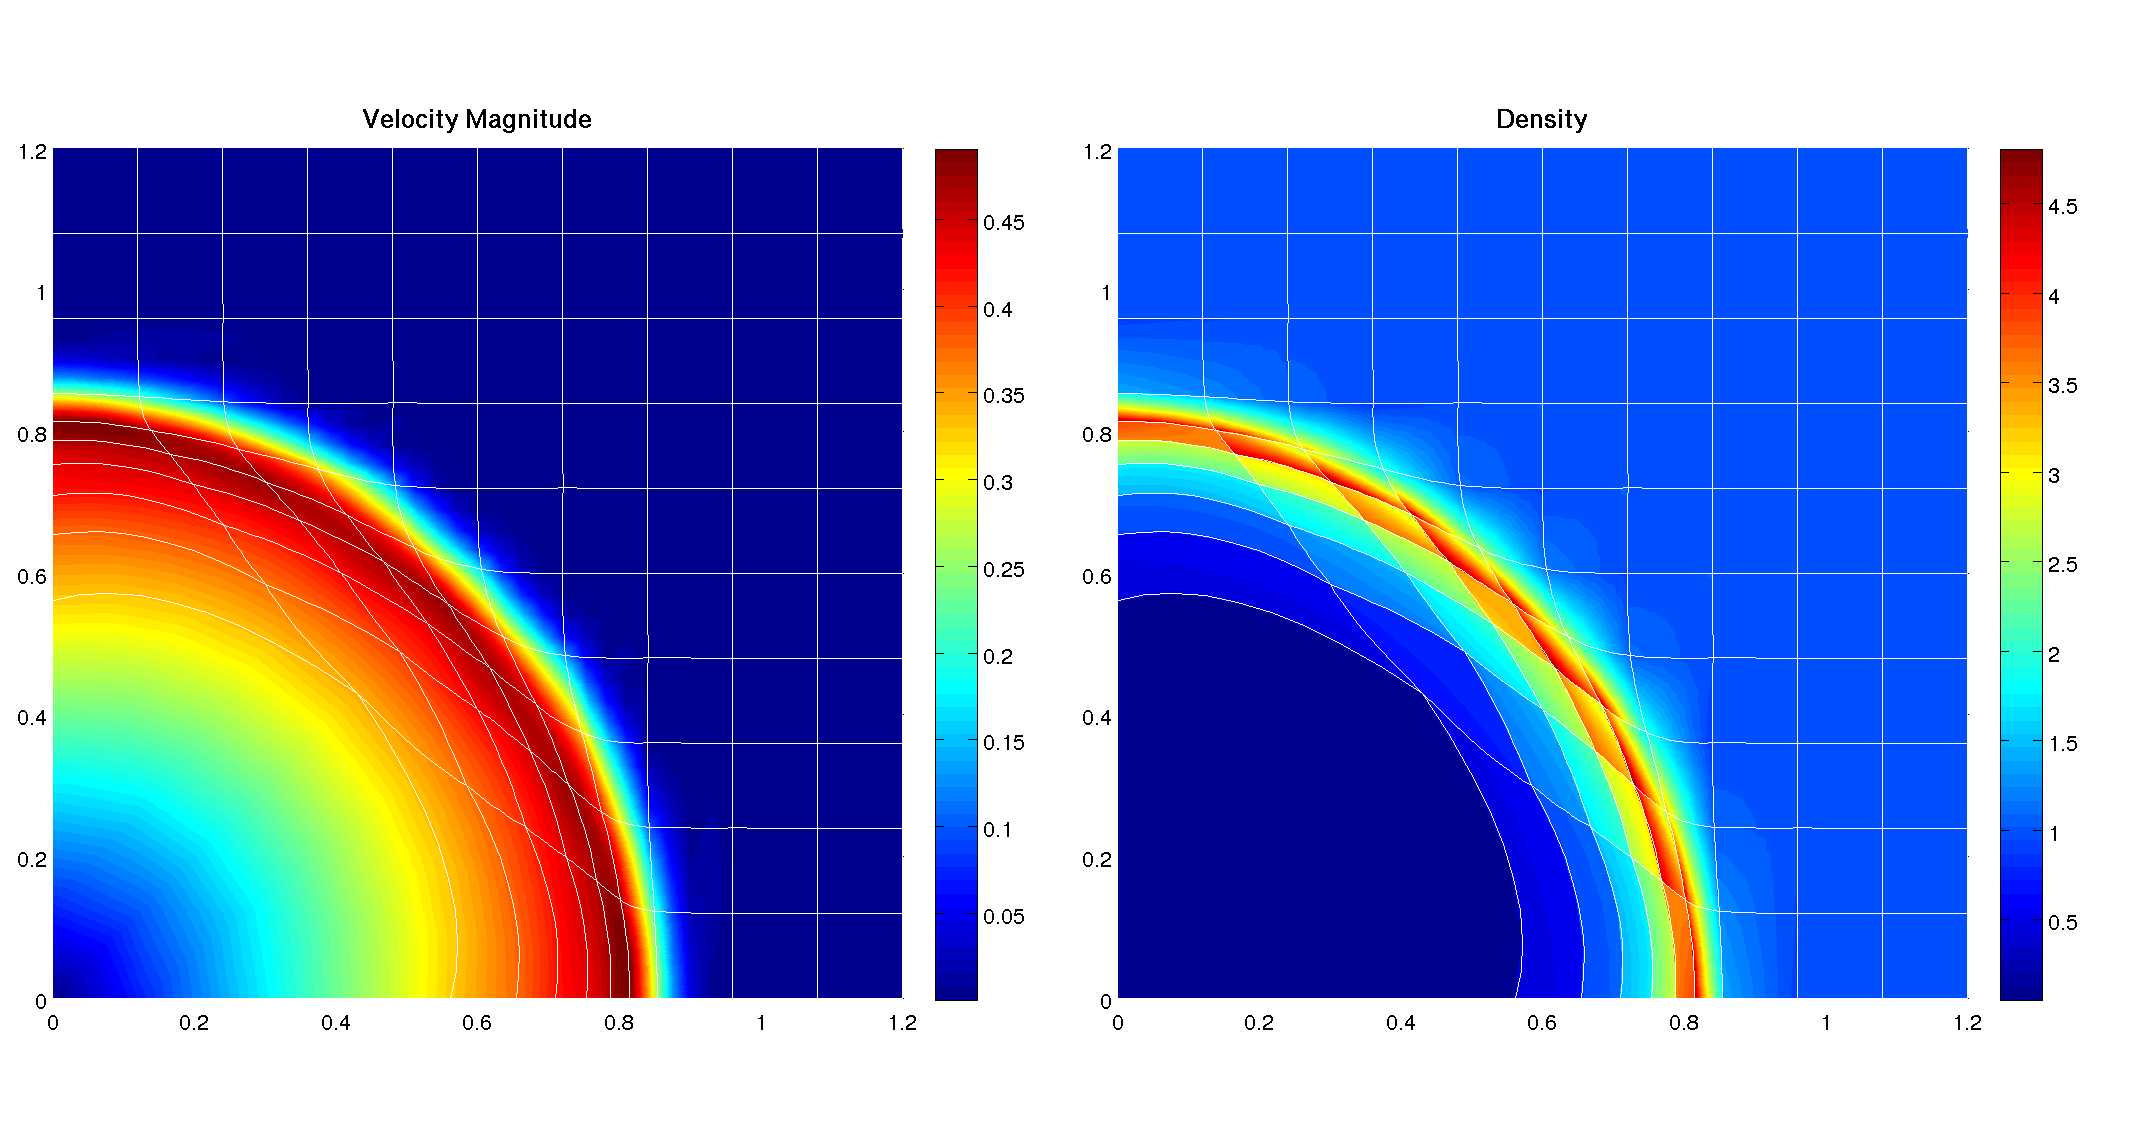
\includegraphics{./Images/SedovAnimation/SedovAnimation_140.png}
    \newframe[1]
    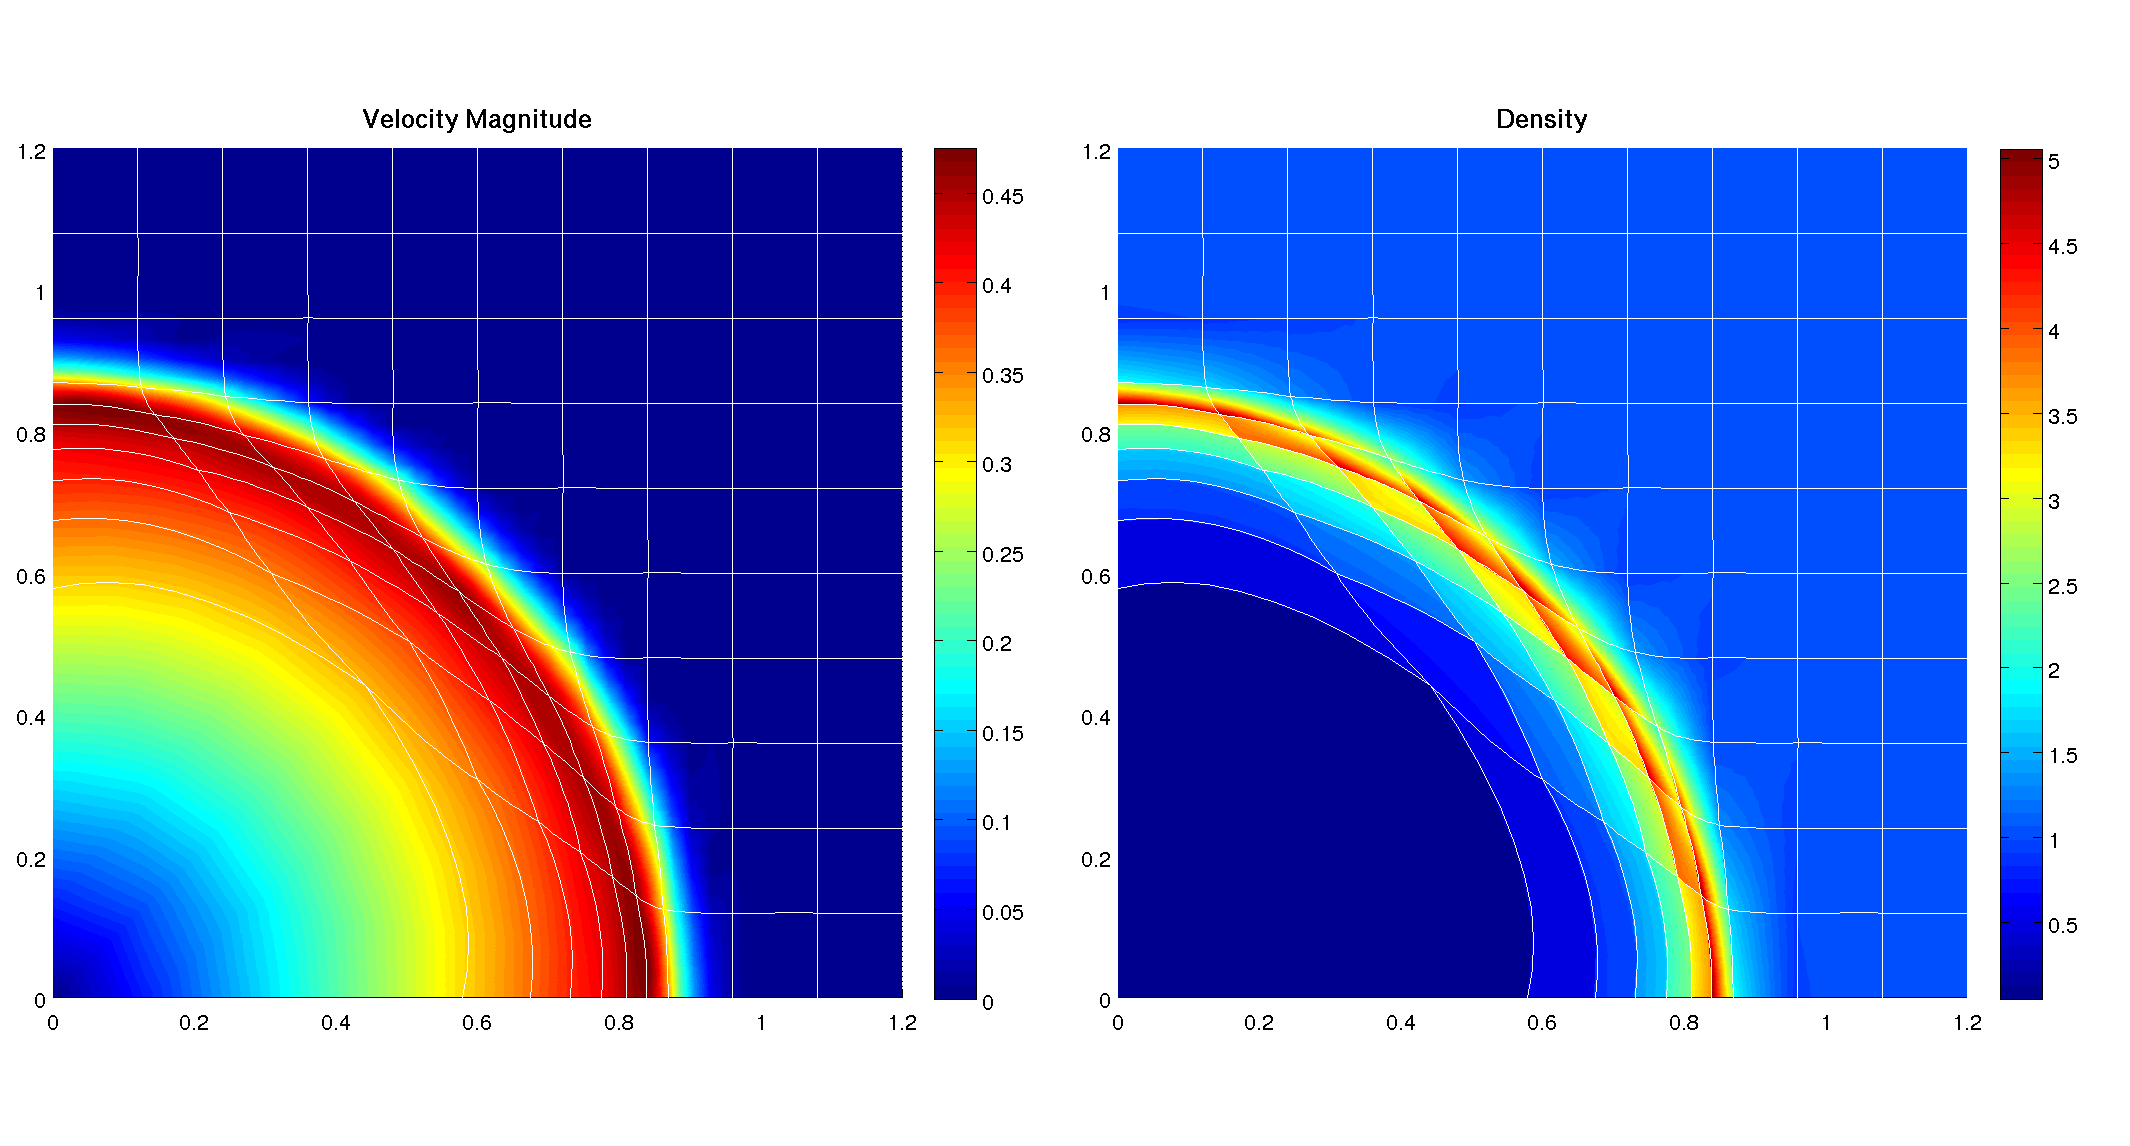
\includegraphics{./Images/SedovAnimation/SedovAnimation_150.png}
    \newframe[1]
    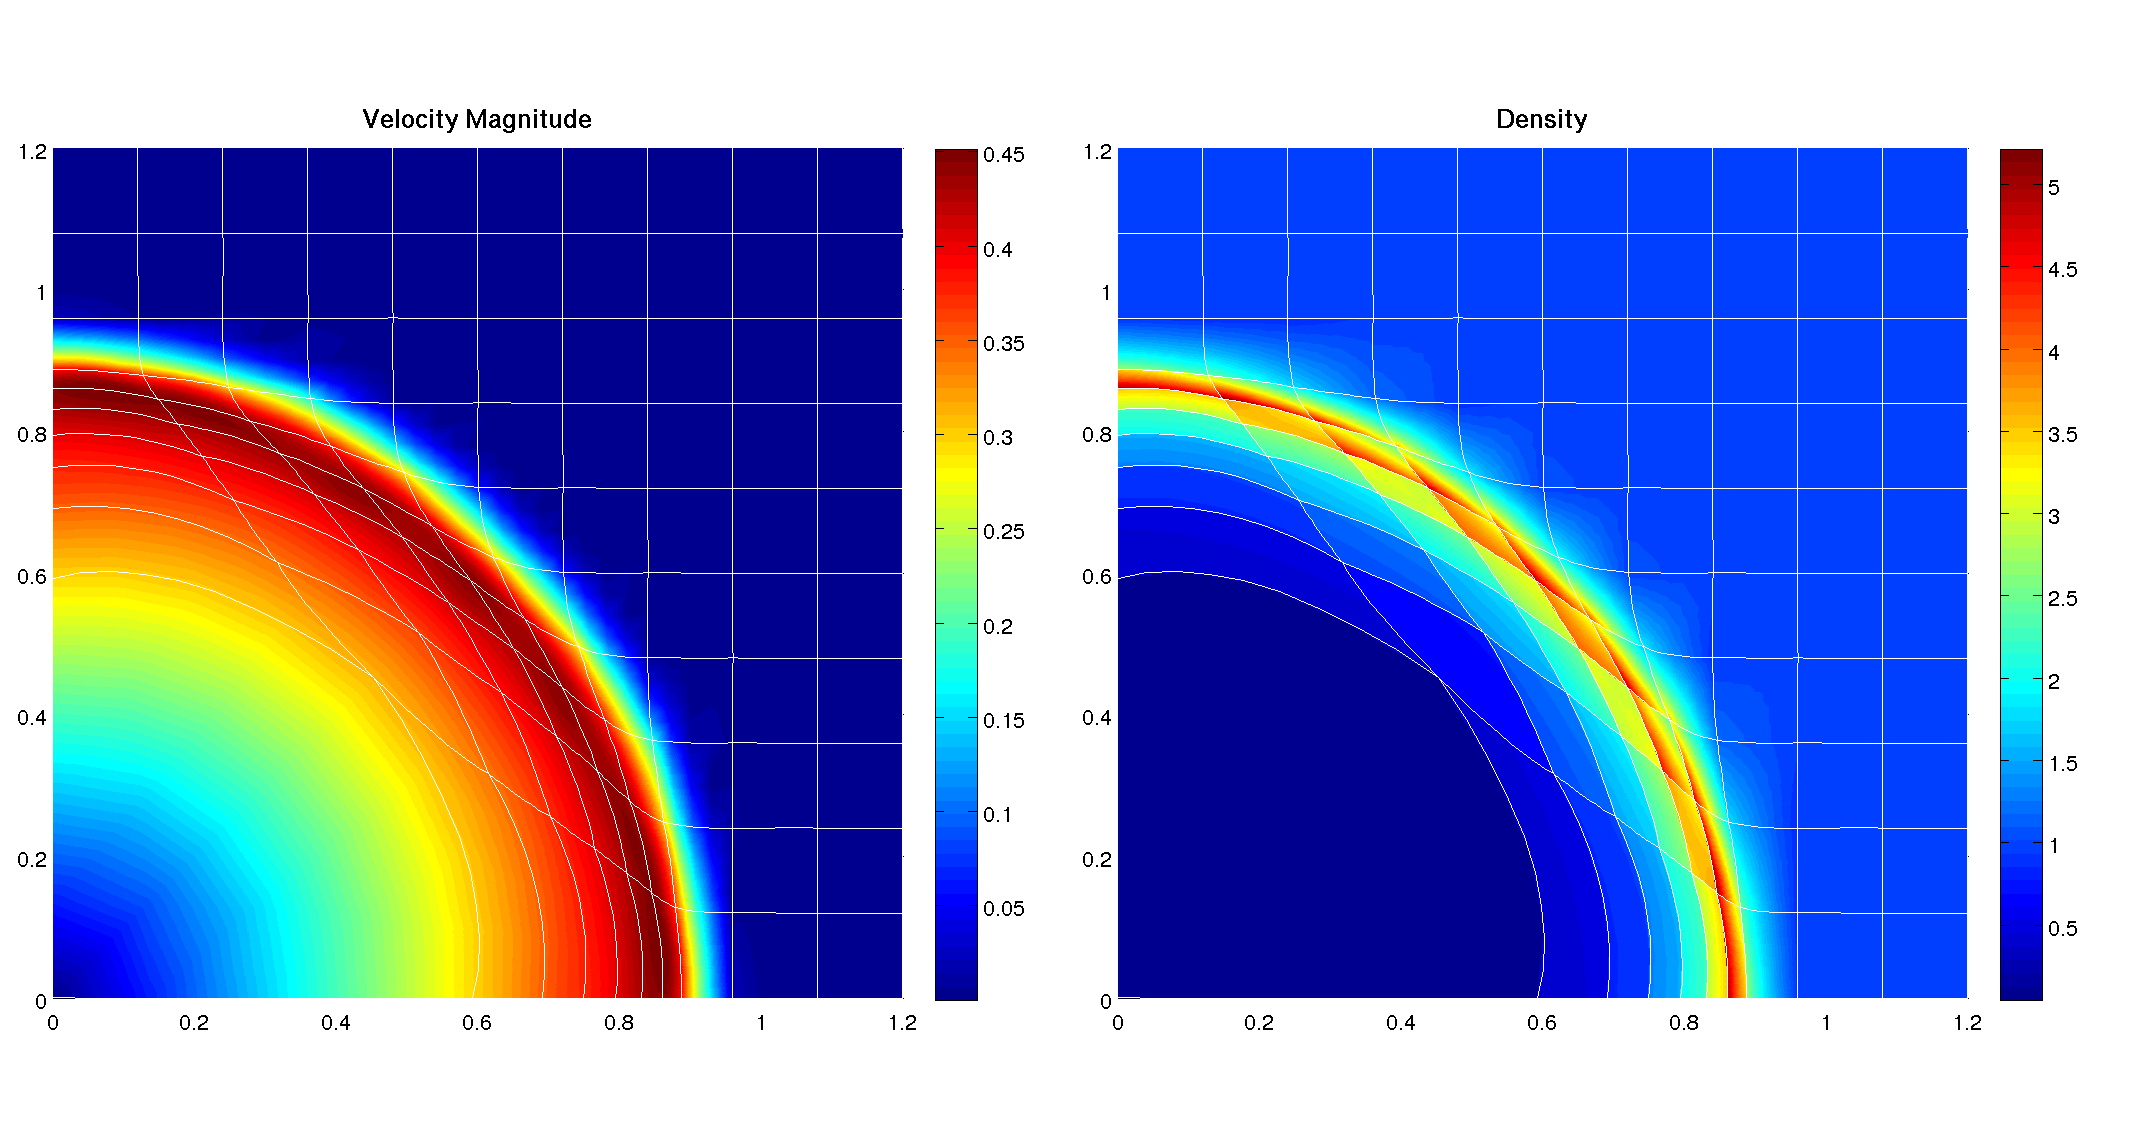
\includegraphics{./Images/SedovAnimation/SedovAnimation_160.png}
    \newframe[1]
    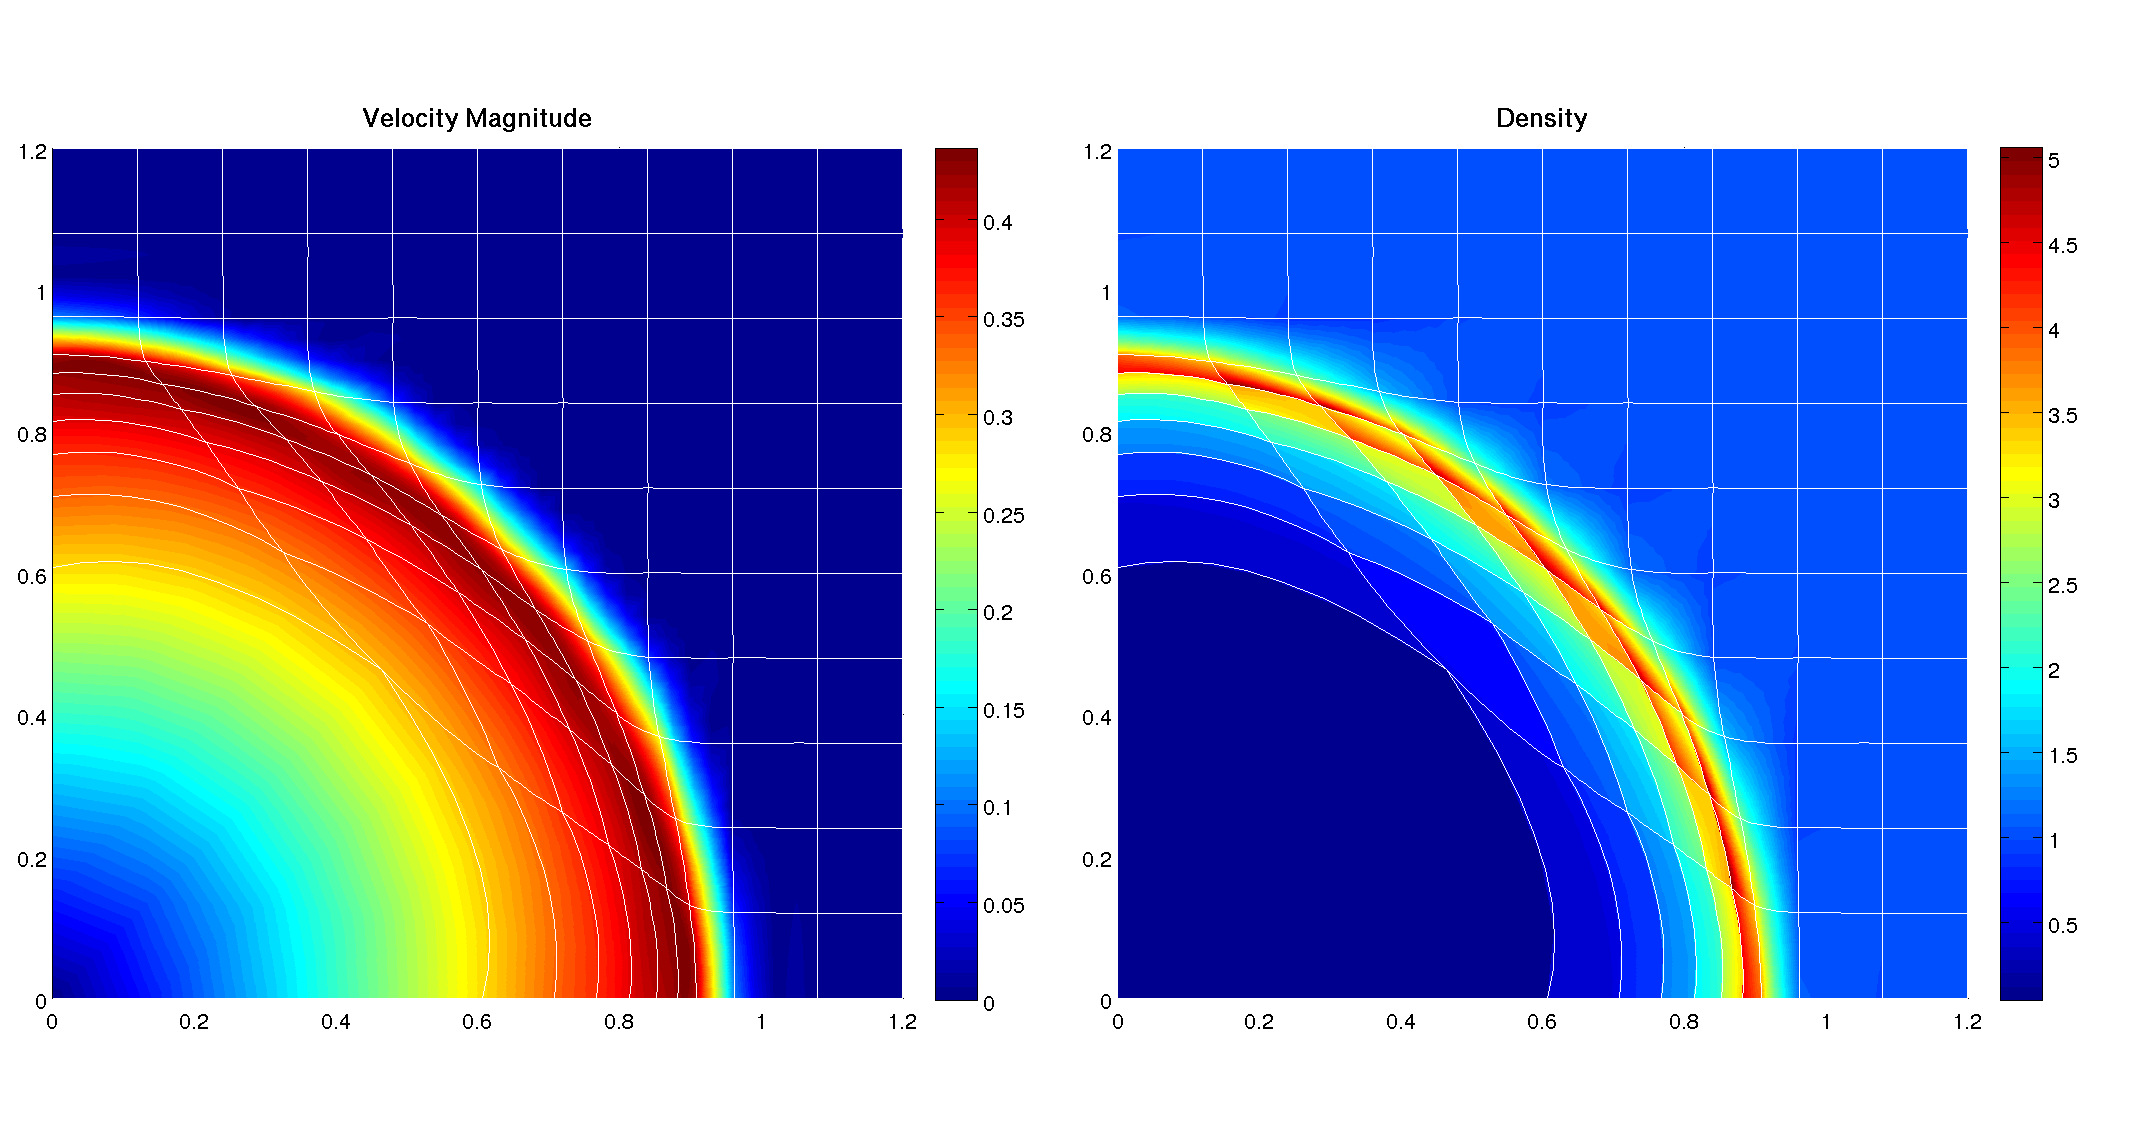
\includegraphics{./Images/SedovAnimation/SedovAnimation_170.png}
    \newframe[1]
    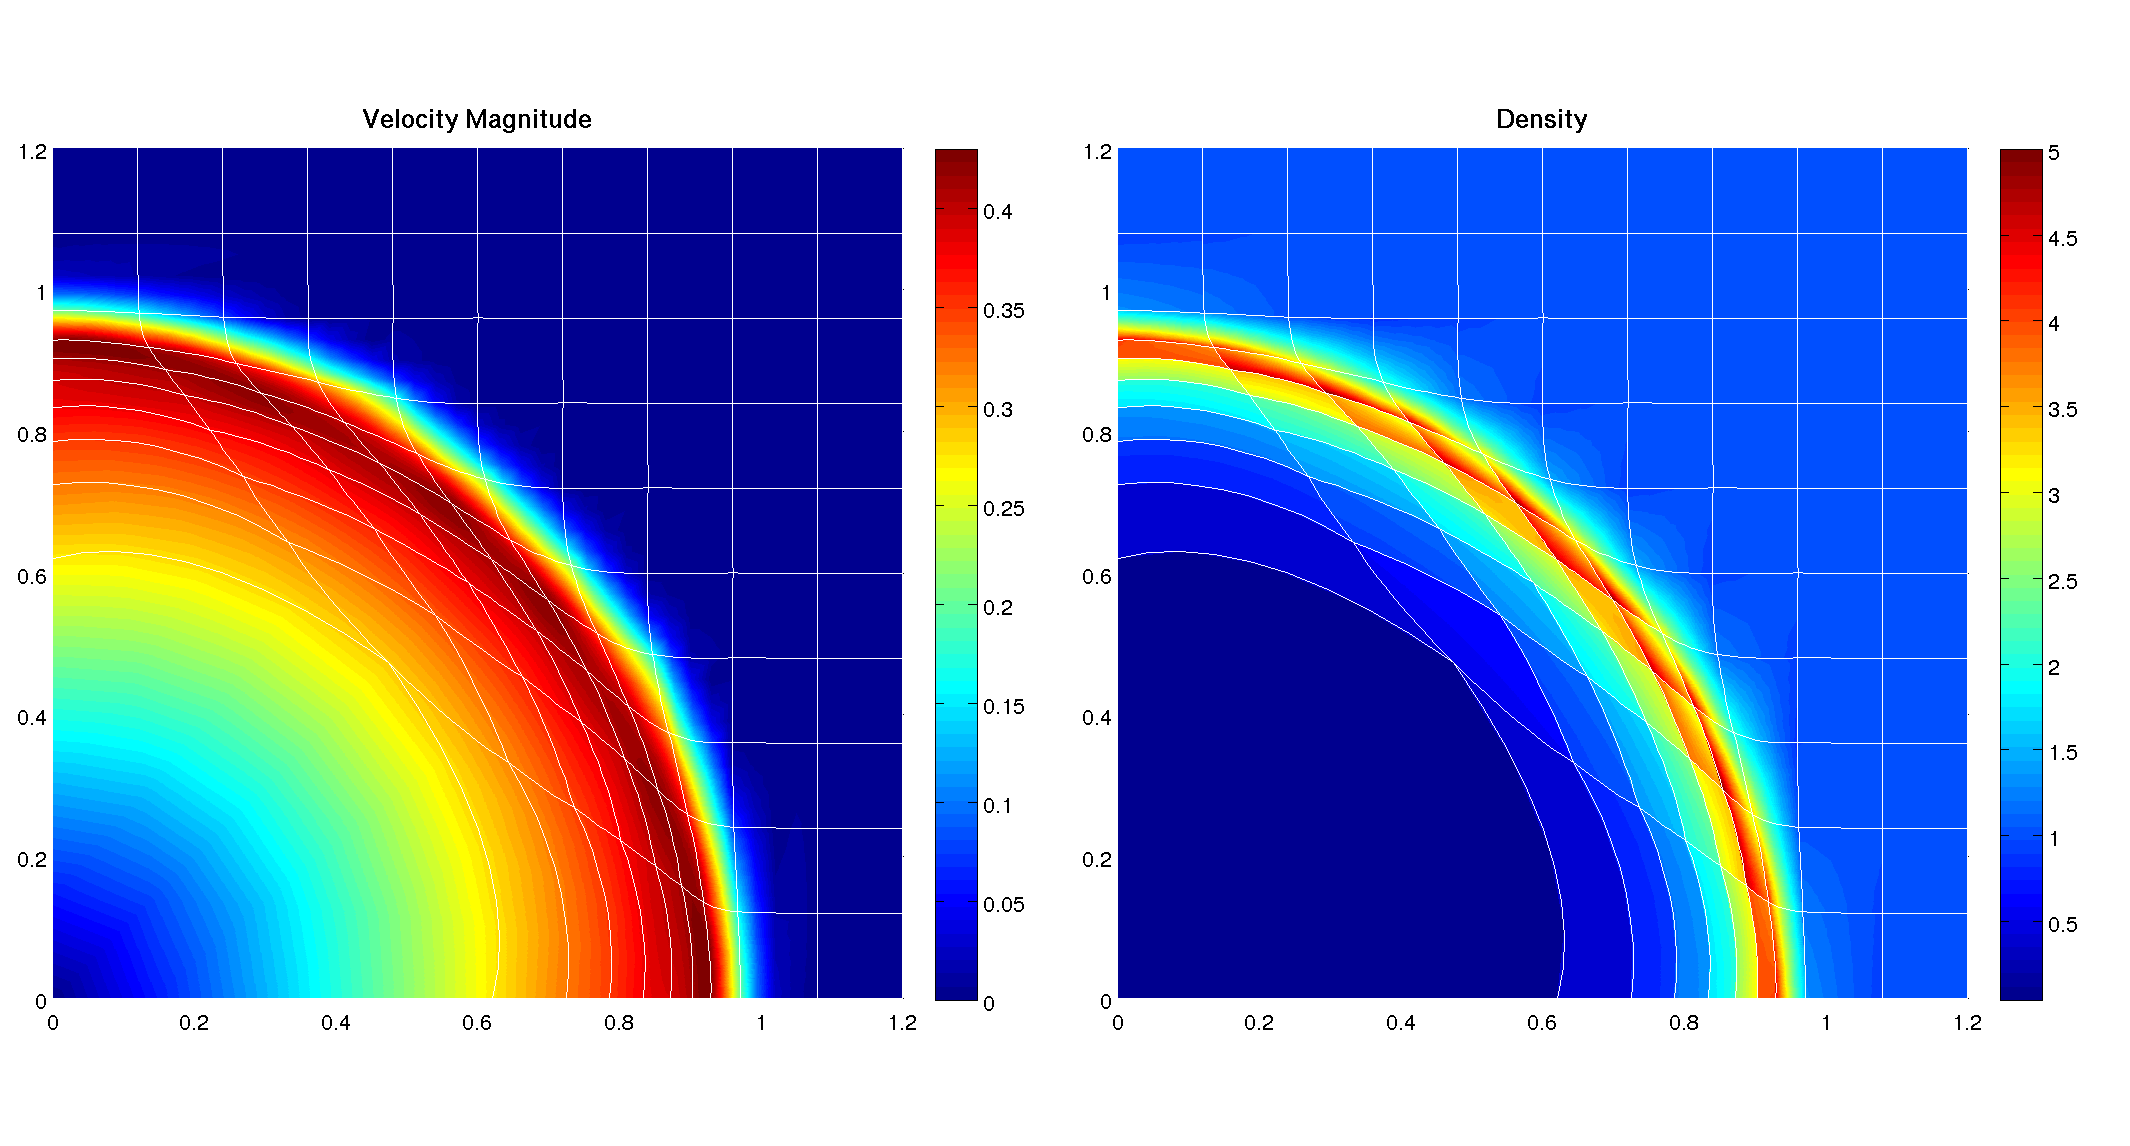
\includegraphics{./Images/SedovAnimation/SedovAnimation_180.png}
    \newframe[1]
    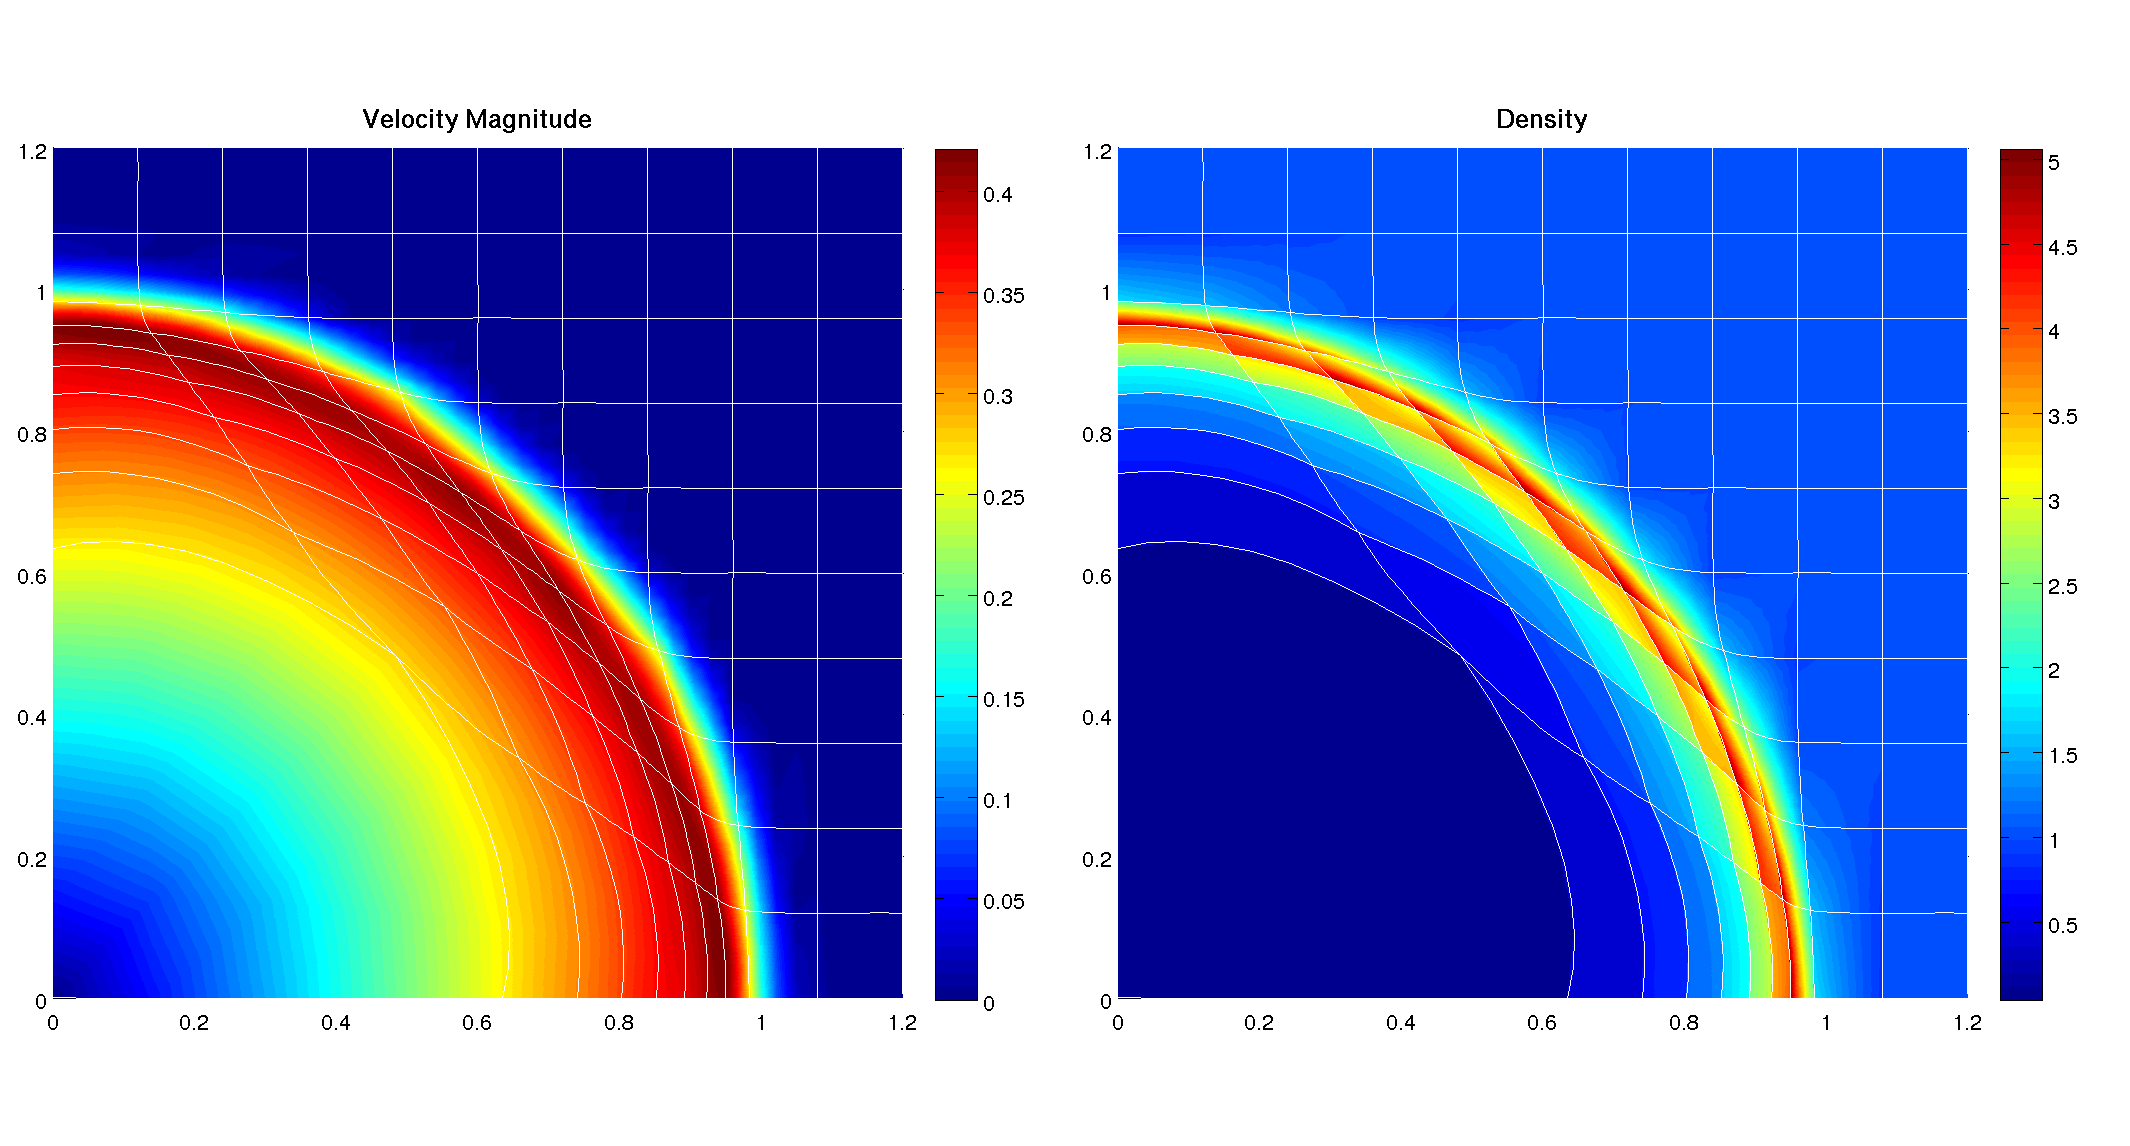
\includegraphics{./Images/SedovAnimation/SedovAnimation_190.png}
    \newframe[1]
    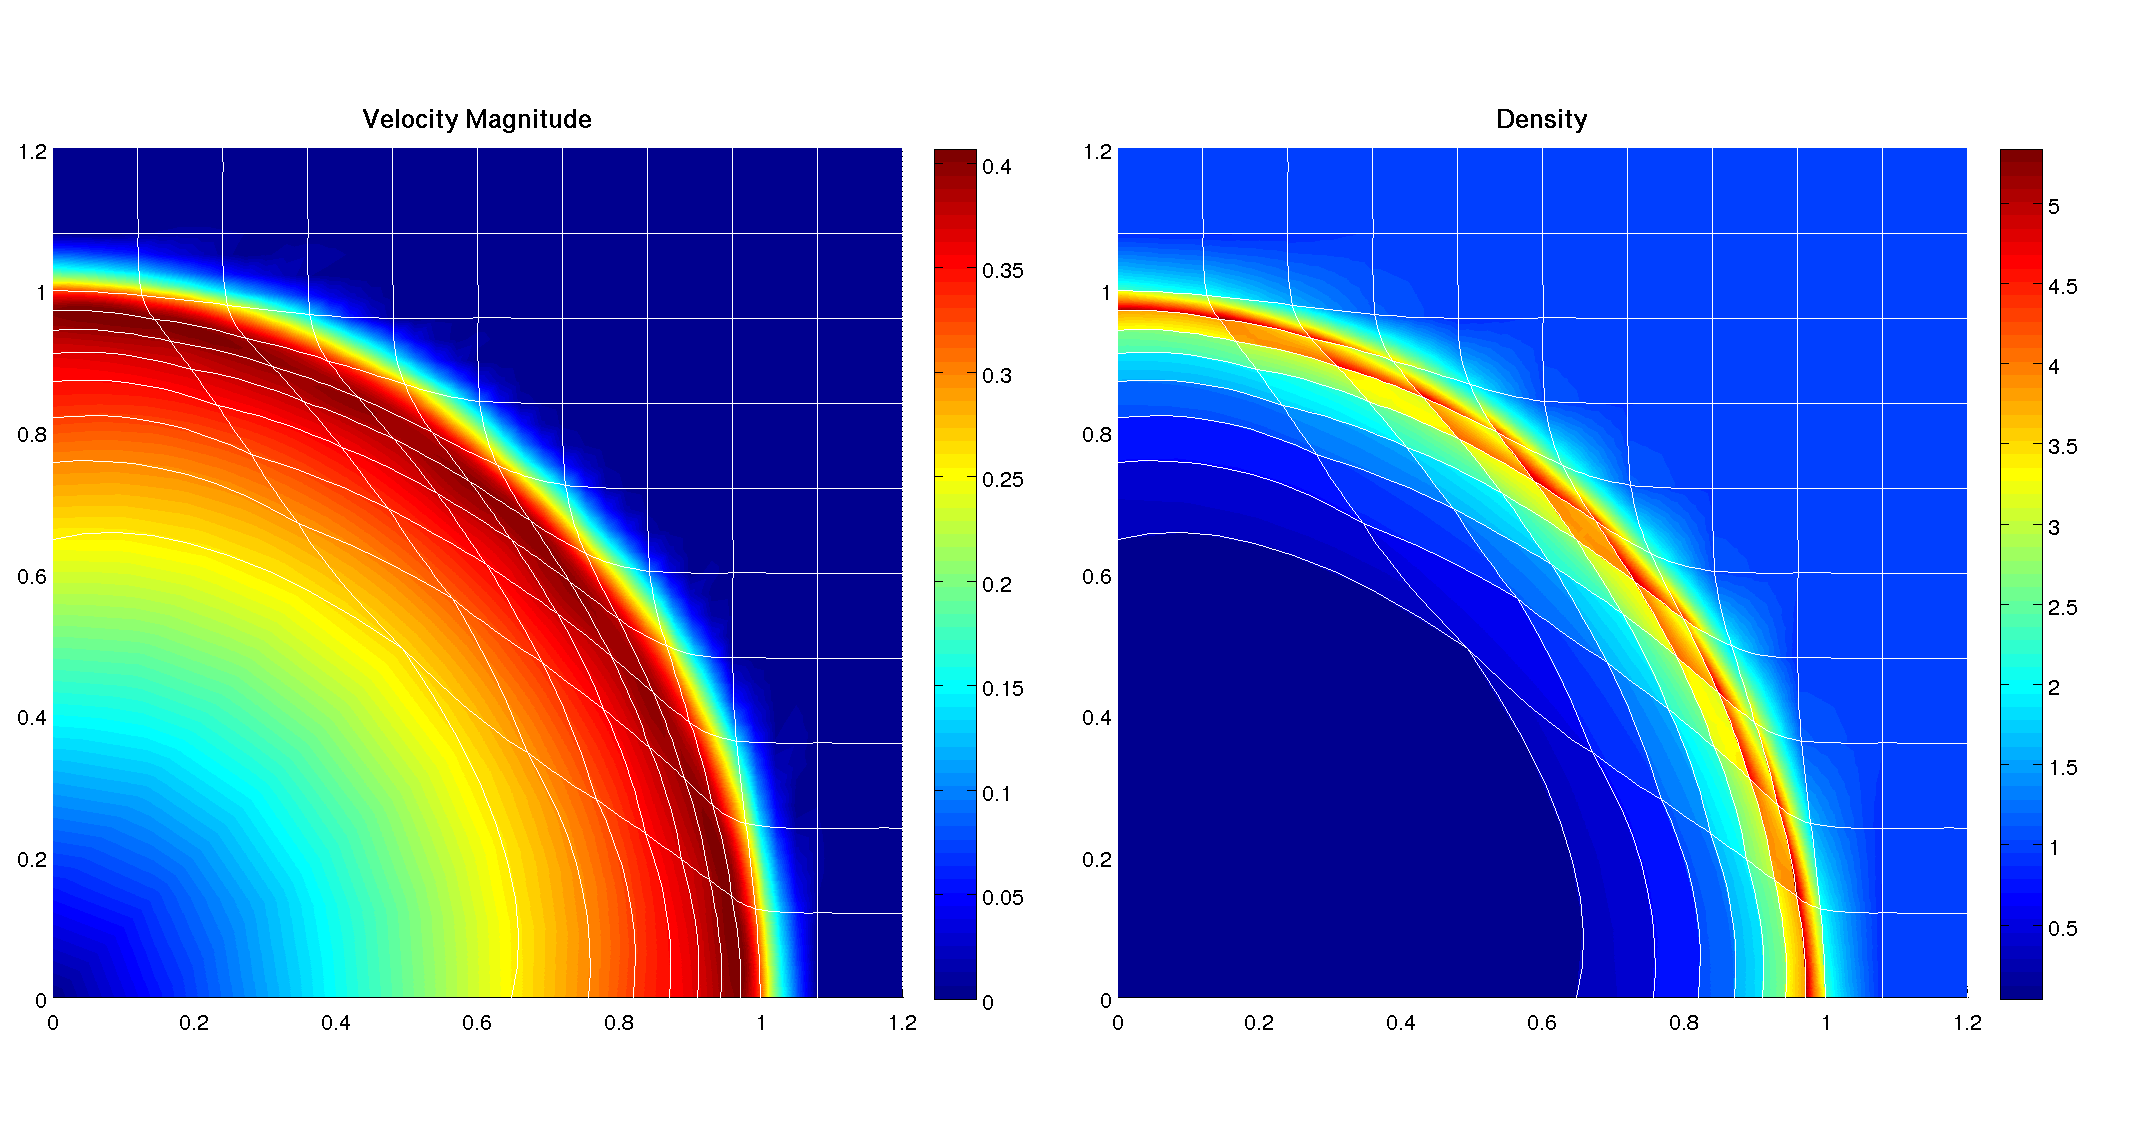
\includegraphics{./Images/SedovAnimation/SedovAnimation_200.png}
    \end{animateinline}
\end{figure}
\end{frame}

\begin{frame}[shrink=5]
 \frametitle{Curved Geometries}
 
 Finite element basis functions are defined on a reference (unit) zone. To compute quantities on an arbitrary mesh zone, we use the Jacobian matrix  which defines the geometric transformation (or mapping) from reference space: 

 \smallskip 
 \begin{columns}
  \begin{column}{0.3\textwidth}
  \centering
  \textcolor{red}{\underline{Reference Space:}}
   \begin{figure}[h!]
    \centering
    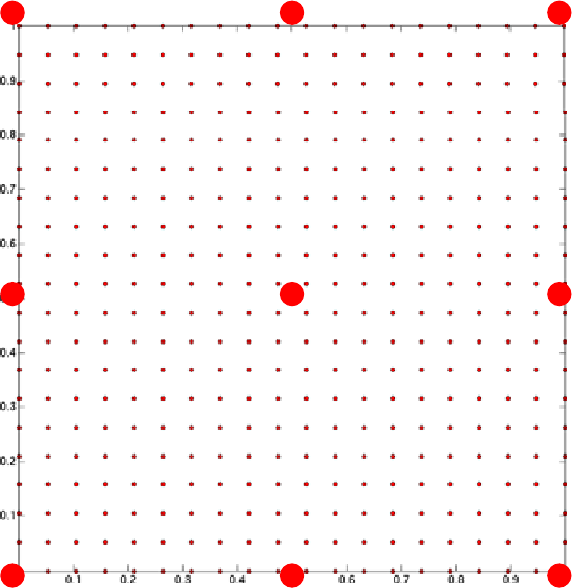
\includegraphics[width=1.0\textwidth,keepaspectratio=true]{./Images/refSpace.png}
    \end{figure}
    \centering
    \fcolorbox{red}{white}{$\phi(\hat{\vec{x}})$} 
    
    \fcolorbox{red}{white}{$\vec{\nabla}\phi(\hat{\vec{x}})$}

  \end{column}
  \begin{column}{0.3\textwidth}
   \begin{figure}[h!]
    \centering
    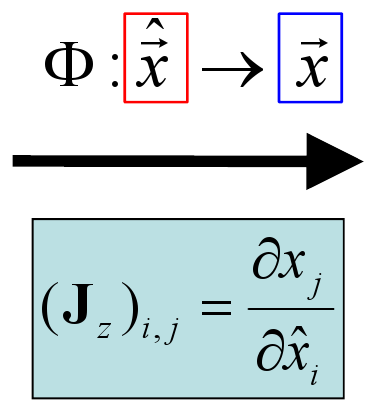
\includegraphics[width=0.6\textwidth,keepaspectratio=true]{./Images/transSpace.png}
    \end{figure}
  \end{column}
  \begin{column}{0.3\textwidth}
  \centering
  \textcolor{blue}{\underline{Physical Space:}}
   \begin{figure}[h!]
    \centering
    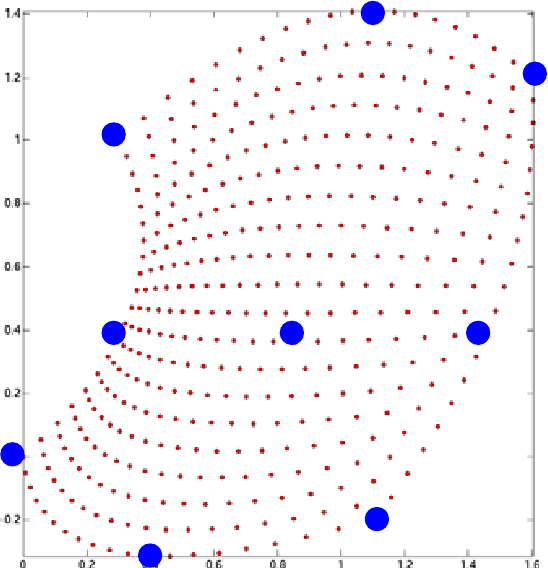
\includegraphics[width=1.0\textwidth,keepaspectratio=true]{./Images/physSpace.png}
    \end{figure}
    \centering
    \fcolorbox{blue}{white}{$\phi(\vec{x})=\hat{\phi}(\Phi^{-1}(\vec{x}))$} \fcolorbox{blue}{white}{$\vec{\nabla}\phi=J_Z^{-1}\vec{\nabla}\hat{\phi}$}
  \end{column}
 \end{columns}
\centering
\begin{block}{}
A standard Q1 mapping gives zones with straight edges, while Q2 mappings produce curved zones.
Note that we can have Q1 elements defined with a Q2 mapping and vice versa. The finite element
reference degrees of freedom are in general different from the nodes of the mapping.
\end{block}
\end{frame}

\begin{frame}
 \frametitle{Basis Functions}
 We approximate each of the continuum fields with a basis function expansion, where the expansion
coefficients are independent of space:
\smallskip

\begin{columns}
 \begin{column}{0.5\textwidth}
 \centering
  \textbf{\underline{Velocity:}} $\vec{v}(\vec{x},t)\approx \displaystyle\sum_i^{N_v} \mathbf{v}_i(t) w_i(\vec{x})$
  
  \textbf{\underline{Internal Energy:}} $e(\vec{x},t)\approx \displaystyle\sum_i^{N_e} \mathbf{e}_i(t) \theta_i(\vec{x})$
 \end{column}
 \begin{column}{0.5\textwidth}
 \centering
  \textbf{\underline{Pressure:}} $p(\vec{x},t)\approx \displaystyle\sum_i^{N_p} \mathbf{p}_i(t) \phi_i(\vec{x})$
  
  \textbf{\underline{Density:}} $\rho(\vec{x},t)\approx \displaystyle\sum_i^{N_{\rho}} \mathbf{\rho}_i(t) \psi_i(\vec{x})$
 \end{column}
\end{columns}
Our formulation is general; we are free to choose various types of basis functions. However, stability
requires that certain choices are not independent$^{[1]}$ (e.g. pressure and velocity.)
\begin{columns}
 \begin{column}{0.3\textwidth}
  \begin{figure}[h!]
    \centering
    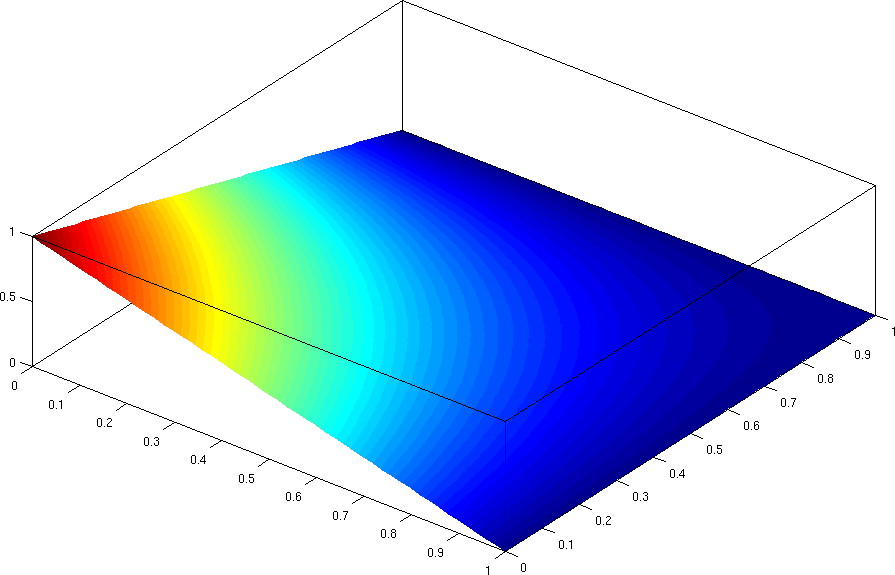
\includegraphics[width=1.0\textwidth,keepaspectratio=true]{./Images/Q1Basis.png}
    \end{figure}
    \centering
    \small{Q1 (Bi-Linear) basis function

    4 DOF per Quad}
 \end{column}
 \begin{column}{0.3\textwidth}
  \begin{figure}[h!]
    \centering
    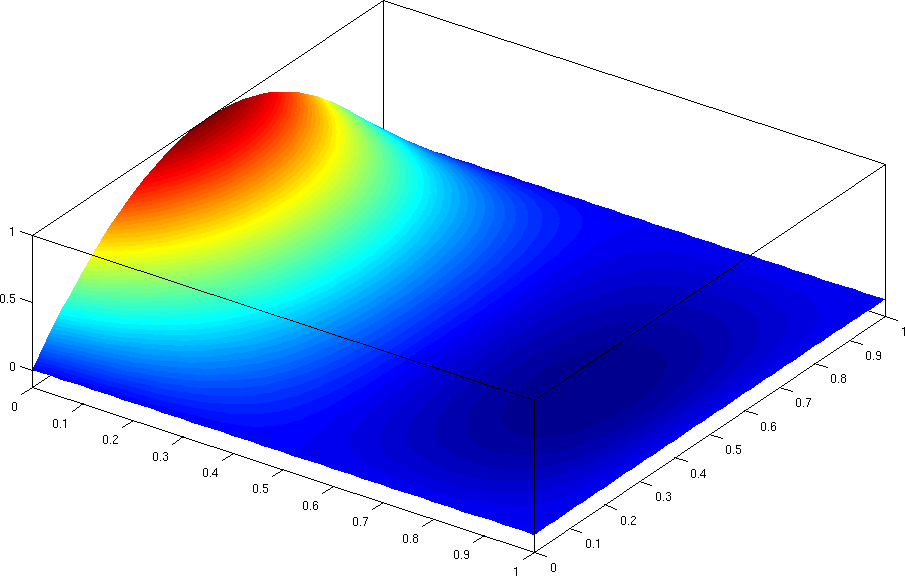
\includegraphics[width=1.0\textwidth,keepaspectratio=true]{./Images/Q2Basis.png}
    \end{figure}
    \centering
    \small{Q2 (Bi-Quadratic) basis function

    9 DOF per Quad}
 \end{column}
 \begin{column}{0.3\textwidth}
  \begin{figure}[h!]
    \centering
    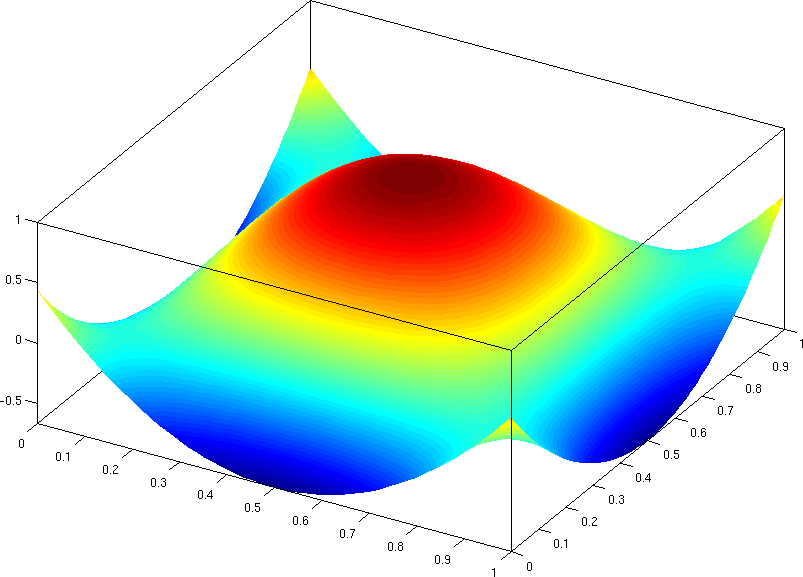
\includegraphics[width=1.0\textwidth,keepaspectratio=true]{./Images/Q2dBasis.png}
    \end{figure}
    \centering
    \small{Q2 basis function with degrees of freedom at the 9 Gauss-Legendre quadrature points}
 \end{column}
\end{columns}
\tiny{[1] See for example: D. Arnold et. al., “Differential Complexes and stability of Finite Element Methods”, 2005.}
\end{frame}


\begin{frame}
 \frametitle{Semi-Discrete Momentum Conservation}
 To derive a semi-discrete momentum conservation law, we begin with a variational formulation:
\[
 \rho \dfrac{\mathrm{d}\vec{v}}{\mathrm{d}t}=-\vec{\nabla} p \quad \Longrightarrow \quad
 \int_{\tilde{\Omega}(t)} \left(\rho\dfrac{\mathrm{d}\vec{v}}{\mathrm{d}t}\right)\cdot \vec{w'}
 =\int_{\tilde{\Omega}(t)} (\vec{\nabla} p) \cdot \vec{w'} \quad = \quad
 \int_{\tilde{\Omega}(t)} p(\vec{\nabla} \cdot \vec{w'}) - \int_{\partial \tilde{\Omega}(t)} p(\vec{w'} \cdot \hat{n}) 
\]
\vspace{-2ex}
\begin{columns}
\begin{column}{0.5\textwidth}
\hspace*{3ex}\parbox{30ex}{\centering \tiny{
Multiply by vector valued test

function, integrate over 

computational mesh}}
\end{column}
\begin{column}{0.5\textwidth}
\hspace*{-5ex}\parbox{30ex}{\centering \tiny{
Perform integration 

by parts
}}
\end{column}
\end{columns}
Inserting our basis function expansions and applying Galerkin’s method by picking the velocity basis
as the test function yields the following linear system of equations:
\begin{columns}
 \begin{column}{0.4\textwidth}
  \[
    \int_{\tilde{\Omega}(t)} \left(\rho\sum_i\frac{\mathrm{d}v_i}{\mathrm{d}t}\vec{w_i}\right)\cdot\vec{w_j}
    =\int_{\tilde{\Omega}(t)} \sum_ip_i\phi_i(\vec{\nabla}\cdot\vec{w_j})
  \]
 \end{column}
 \begin{column}{0.2\textwidth}
 \centering
 \tiny{Write in matrix / vector form}\smallskip
 
  \scalebox{4}{$\longrightarrow$}
 \end{column}
 \begin{column}{0.175\textwidth}
 \begin{block}{}
 \centering
 \Large{$\mathbf{M}\dfrac{\mathrm{d}\mathbf{v}}{\mathrm{d}t}=\mathbf{D}^T\mathbf{p}$}
 \end{block}
 \end{column}
\end{columns}
The \textbf{\underline{Mass}} and \textbf{\underline{Derivative}} matrices are computed zone by zone and assembled to form global systems:
\begin{columns}[T]
\begin{column}{0.3\textwidth}
\centering
  \begin{block}{}
    \Large{$(\mathbf{M}_z)_{ij}=\int_{\tilde{\Omega}(t)} \rho(\vec{w_i}\cdot\vec{w_j})$}
  \end{block}
\tiny{The symmetric
positive definite mass
matrix describes how matter is
distributed in space}
 \end{column}
 \begin{column}{0.3\textwidth}
 \centering
  \begin{block}{}
    \Large{$(\mathbf{D}_z)_{ij}=\int_{\tilde{\Omega}(t)} \phi_i(\vec{\nabla}\cdot\vec{w_j})$}
  \end{block}
\tiny{The rectangular derivative matrix maps between
pressure and velocity spaces. This matrix is a
discrete version of the Div operator. Its adjoint
(transpose) is the Grad operator}
 \end{column}
\end{columns}
\end{frame}

 
\begin{frame}
  \frametitle{Computing Mass and Derivative Matrices}
  In practice, we compute the mass and derivative matrices by integrating over the reference volume
  using a change of variables:
  \[
  \int_{\Omega(t)} f = \int_{\tilde{\Omega}(t)}(f\circ\Phi)|{\mathbf{J}_z}|
  \]
  The integrals are computed using Gaussian quadrature of a specified order. For certain integrands and
  quadrature rules, this can be computed exactly:
  \[
  \int_{\tilde{\Omega}(t)}(f\circ\Phi)|{\mathbf{J}_z}|\approx
  \sum_{n=1}^{N_q}\alpha_n\left\{f\circ\Phi)|{\mathbf{J}_z}|\right\}_{\hat{\vec{x}}=\hat{\vec{q_n}}}
  \]
  \begin{columns}[T]
  \begin{column}{0.2\textwidth}
    \begin{figure}[h!]
      \centering
      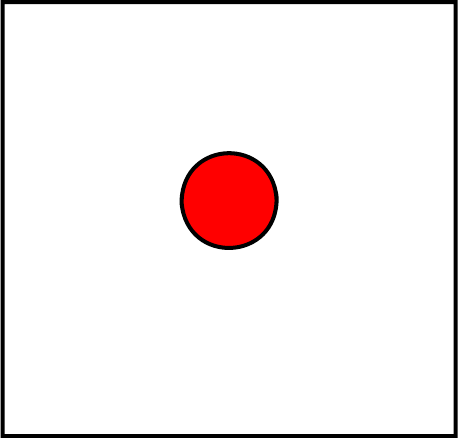
\includegraphics[width=1.0\textwidth,keepaspectratio=true]{./Images/quad1.png}
      \end{figure}
      \centering
      \tiny{2D Order 1
	Gauss-Legendre rule
	(exact for Q1)}
  \end{column}
  \begin{column}{0.2\textwidth}
    \begin{figure}[h!]
      \centering
      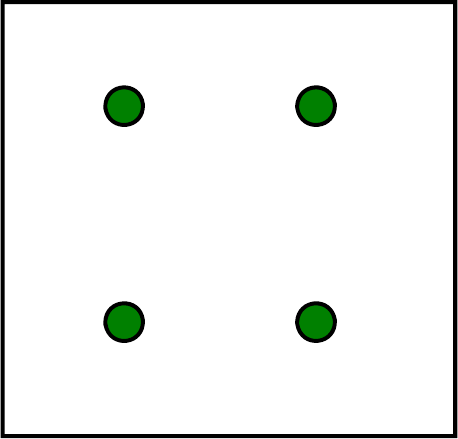
\includegraphics[width=1.0\textwidth,keepaspectratio=true]{./Images/quad2.png}
      \end{figure}
      \centering
      \tiny{2D Order 2
	Gauss-Legendre rule
	(exact for Q3)}
  \end{column}
  \begin{column}{0.2\textwidth}
    \begin{figure}[h!]
      \centering
      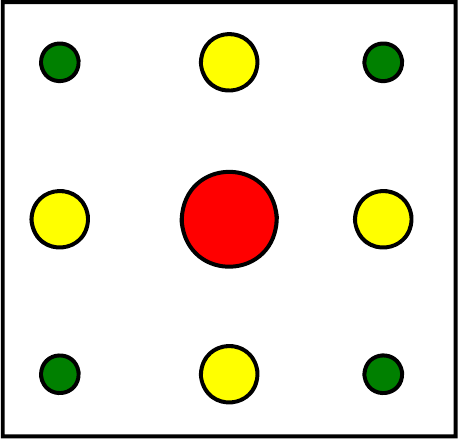
\includegraphics[width=1.0\textwidth,keepaspectratio=true]{./Images/quad3.png}
      \end{figure}
      \centering
      \tiny{2D Order 3
	Gauss-Legendre rule
	(exact for Q5)}
  \end{column}
  \begin{column}{0.2\textwidth}
    \begin{figure}[h!]
      \centering
      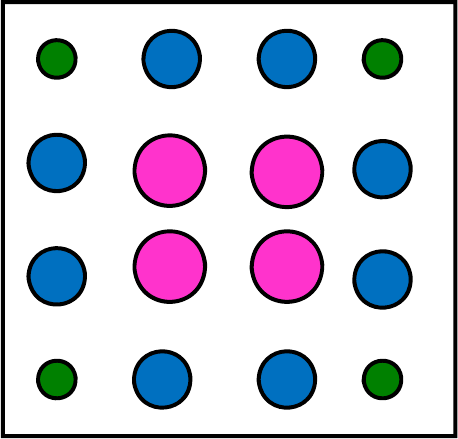
\includegraphics[width=1.0\textwidth,keepaspectratio=true]{./Images/quad4.png}
      \end{figure}
      \centering
      \tiny{2D Order 4
	Gauss-Legendre rule
	(exact for Q7)}
  \end{column}
  \end{columns}
\end{frame}

\begin{frame}
 \frametitle{Semi-Discrete Mass Conservation}
We define the zonal mass moments in a natural manner: \quad $\displaystyle{\mathbf{m}_{z,i}=\int\limits_{\Omega_z(t)} \rho \psi_i}$

The Lagrangian description requires that: \quad $\dfrac{\mathrm{d}\mathbf{m}_{z,i}}{\mathrm{d}t}=0$

From the representation: \quad $\rho(\vec{x},t)\approx \displaystyle{\sum_i} \mathbf{\rho}_i(t) \psi_i(\vec{x})$ \quad it follows that: \quad
$\displaystyle{\mathbf{m}_{z,i}=\sum_j\mathbf{\rho}_{z,j}\int\limits_{\Omega_z(t)} \psi_i\psi_j}$

In matrix form we have: \quad \colorbox{cyan!30}{$\displaystyle
     \mathbf{m}_z=\mathbf{M}_z^\rho \mathbf{\rho}_z$} \quad where \quad $\displaystyle
     (\mathbf{M}_z^\rho)_{i,j}=\int\limits_{\Omega_z(t)} \psi_i \psi_j$

If we impose the stronger condition: \quad $\dfrac{\mathrm{d}}{\mathrm{d}t}\int\limits_{\Omega(t)}\rho\psi=0$ \quad for \underline{\textbf{any}} function $\psi$

then we obtain the \textcolor{red}{\emph{strong mass conservation principle}}:
\begin{columns}[T]
\begin{column}{0.4\textwidth}
\colorbox{cyan!30}{$
 \rho(t)|\mathbf{J}(t)|=\rho(t_0)|\mathbf{J}(t_0)|$}
\end{column}
\end{columns}

Note that, in general, the density defined by the above equation is \textcolor{red}{\emph{not polynomial}}.

\begin{block}{}\centering
 Note that both generalizations imply the standard zonal mass conservation
\end{block}
\end{frame}

\begin{frame}
 \frametitle{Energy Conservation, EOS, and Artificial Viscosity}
We treat the energy conservation equation in a local manner. Consider the special case of piece-wise
constant internal energies; we have the following semi-discrete energy conservation law: \vspace{-2ex}
\begin{center}
\fcolorbox{black}{cyan!30}{$\displaystyle \mathbf{m}_z\dfrac{\mathrm{d}\mathbf{e}_z}{\mathrm{d}t}=-\mathbf{p}_z\mathbf{D}_z\mathbf{v}_z = -\left(\mathbf{p}_z\mathbf{D}_z\right)\mathbf{v}_z = -\sum_i \; \vec{f}_i \cdot \vec{v}_i$}
\end{center}

\bigskip
The equation of state is evaluated point-wise according to \hspace*{3ex} \fcolorbox{black}{cyan!30}{$\displaystyle p = EOS(\rho,e)$}

\bigskip
Artificial viscosity is added to the corner forces to counteract shock compression
\medskip
\begin{columns}
\begin{column}{0.3\textwidth}
\centering
\fcolorbox{black}{cyan!30}{$\displaystyle \vec{f}_{Q} = \vec{\nabla}\cdot\left(\mu\vec{\nabla}\;\vec{v}\right)$}
\end{column}
\begin{column}{0.2\textwidth}
\centering
\footnotesize{Variational Formulation} \\
\Large{$\Longrightarrow$}
\end{column}
\begin{column}{0.4\textwidth}
\centering
\fcolorbox{black}{cyan!30}{$\displaystyle \vec{f}_{Q} =-\int_\Omega \mu\vec{\nabla}\vec{v}_z\cdot\vec{\nabla}\phi=-\mathbf{S}_z\mathbf{v}_z$}
\end{column}
\end{columns}

\medskip
 where \hspace*{3ex} \fcolorbox{black}{cyan!30}{$\displaystyle (\mathbf{S}_z)_{i,j} = \int_{\tilde \Omega}\rho_z\mu_z\left(\mathbf{J}_z^{-1}\vec{\nabla}\phi_i\right)\cdot\left(\mathbf{J}_z^{-1}\vec{\nabla}\phi_j\right)|\mathbf{J}_z|$}

\medskip
The viscosity coefficient has adjustable linear term to control oscillations and quadratic term to handle shock smoothing. Artificial viscosity is usually turned off in expansion.
\end{frame}

% \begin{frame}
%  \frametitle{Fully-Discrete Finite Element Approximation: Discrete Energy Conservation}
% \end{frame}



\begin{frame}
 \frametitle{Mixed Finite Elements}
 \begin{figure}[h!]
  \centering
  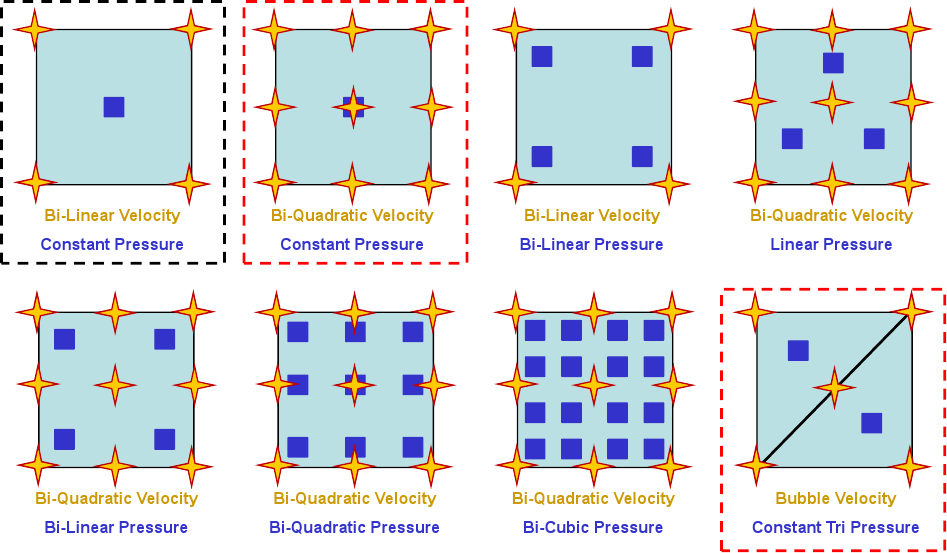
\includegraphics[height=0.8\textheight,keepaspectratio=true]{./Images/mixedElements.png}
  % lagHydro.png: 434x611 pixel, 107dpi, 10.27x14.45 cm, bb=0 0 291 410
  \end{figure}
\end{frame}

\begin{frame}
 \frametitle{High Order Methods Using the Q2 Basis}
 \begin{columns}
  \begin{column}{0.35\textwidth}
{\footnotesize
   For each Q2 zone, we track 9 independent vertices (coordinates, velocities, accelerations etc …) which define the quadratic mapping from reference space to physical space. This mapping is defined using the Q2 Jacobian matrix, which is a function: }
   
\bigskip
\tiny{\texttt{
J(x,y) =  [(y - 1)(2y - 1)(4x - 3)X1 \\
\hspace*{10ex}     + (y- 1)(2y - 1)(4x - 1)X2 \\
\hspace*{10ex}     + y(2y - 1)(4x - 1)X3  \\
\hspace*{10ex}     + y(2y- 1)(4x - 3)X4 \\
\hspace*{10ex}     - 4(y - 1)(2y - 1)(2x - 1)X5 \\ 
\hspace*{10ex}     - 4y(y - 1)(4x - 1)X6 \\
\hspace*{10ex}     - 4y(2y - 1)(2x - 1)X7  \\
\hspace*{10ex}     - 4y(y - 1)(4x- 3)X8 \\
\hspace*{10ex}     + 16y(y - 1)(2x - 1)X9 , \\
%
\hspace*{10ex}       (4y - 3)(x - 1)(2x - 1)X1\\  
\hspace*{10ex}     + x(4y - 3)(2x - 1)X2 \\
\hspace*{10ex}     + x(4y - 1)(2x - 1)X3  \\
\hspace*{10ex}     + (4y - 1)(x - 1)(2x - 1)X4 \\
\hspace*{10ex}     - 4x(4y - 3)(x -1)X5  \\
\hspace*{10ex}     - 4x(2y -1)(2x - 1)X6 \\
\hspace*{10ex}     - 4x(4y - 1)(x - 1)X7  \\
\hspace*{10ex}     - 4(2y - 1)(x - 1)(2x - 1)X8 \\
\hspace*{10ex}     + 16x(2y - 1)(x - 1)X9 ]
}}
\vspace*{-4ex}
   
%    \tiny{\texttt{
%     Jmat=[(-4*(y - 1)*(2*y - 1)*(2*x - 1)*X5 + (y - 1)*(2*y - 1)*(4*x - 3)*X1 
%     + (y- 1)*(2*y - 1)*(4*x - 1)*X2 + 16*(y - 1)*(2*x - 1)*X9*y 
%     - 4*(y - 1)*(4*x- 3)*X8*y - 4*(y - 1)*(4*x - 1)*X6*y 
%     - 4*(2*y - 1)*(2*x - 1)*X7*y + (2*y- 1)*(4*x - 3)*X4*y 
%     + (2*y - 1)*(4*x - 1)*X3*y);
%     (-4*(2*y - 1)*(x - 1)*(2*x - 1)*X8 + 16*(2*y - 1)*(x - 1)*X9*x 
%     - 4*(2*y -1)*(2*x - 1)*X6*x + (4*y - 3)*(x - 1)*(2*x - 1)*X1 
%     - 4*(4*y - 3)*(x -1)*X5*x + (4*y - 3)*(2*x - 1)*X2*x 
%     + (4*y - 1)*(x - 1)*(2*x - 1)*X4 -4*(4*y - 1)*(x - 1)*X7*x 
%     + (4*y - 1)*(2*x - 1)*X3*x)];}}
  \end{column}
  \begin{column}{0.6\textwidth}
   \begin{columns}[t]
   \begin{column}{0.5\textwidth}
   \begin{center}
    \tiny{\textcolor{red}{Points in reference space}}
    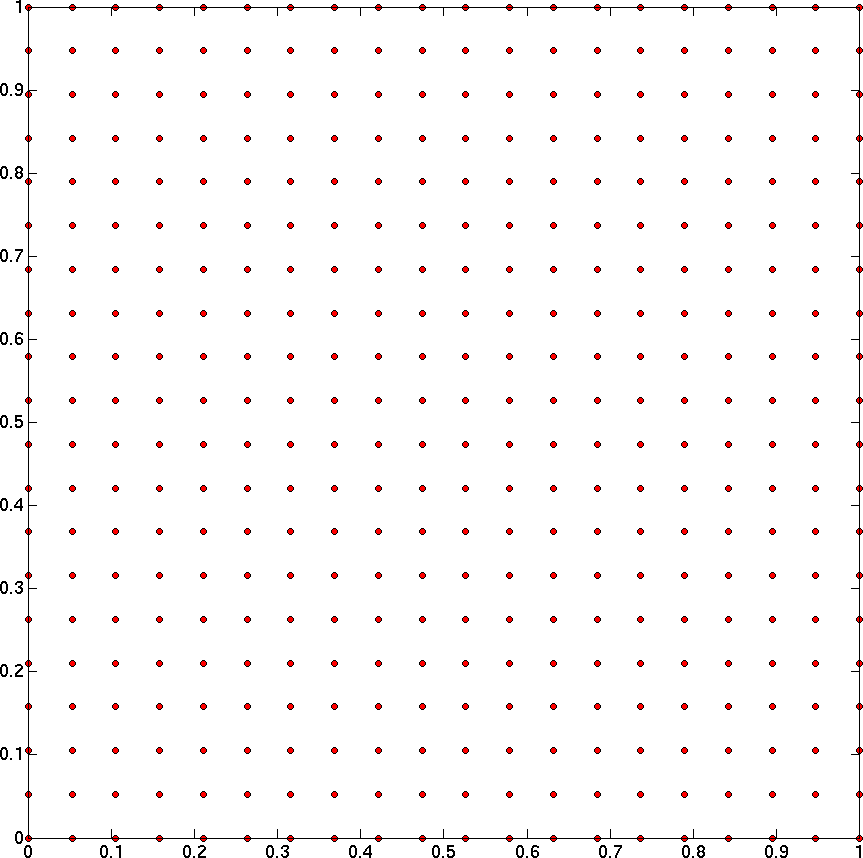
\includegraphics[height=0.4\textheight,keepaspectratio=true]{./Images/Q2Points_Reference.png}
    
    \medskip
    \tiny{\textcolor{red}{Basis function in reference space}}
    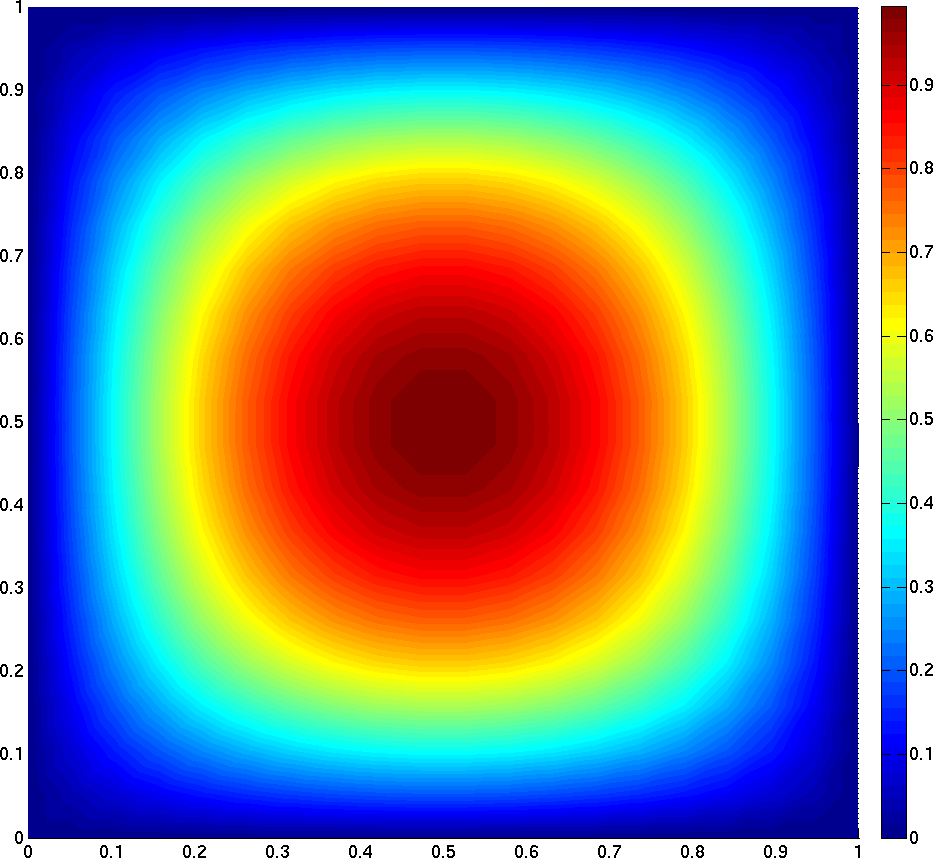
\includegraphics[height=0.4\textheight,keepaspectratio=true]{./Images/Q2Basis_Reference.png}
   \end{center}
   \end{column}
   \begin{column}{0.5\textwidth}
   \begin{center}
    \tiny{\textcolor{blue}{Points in physical space}}
    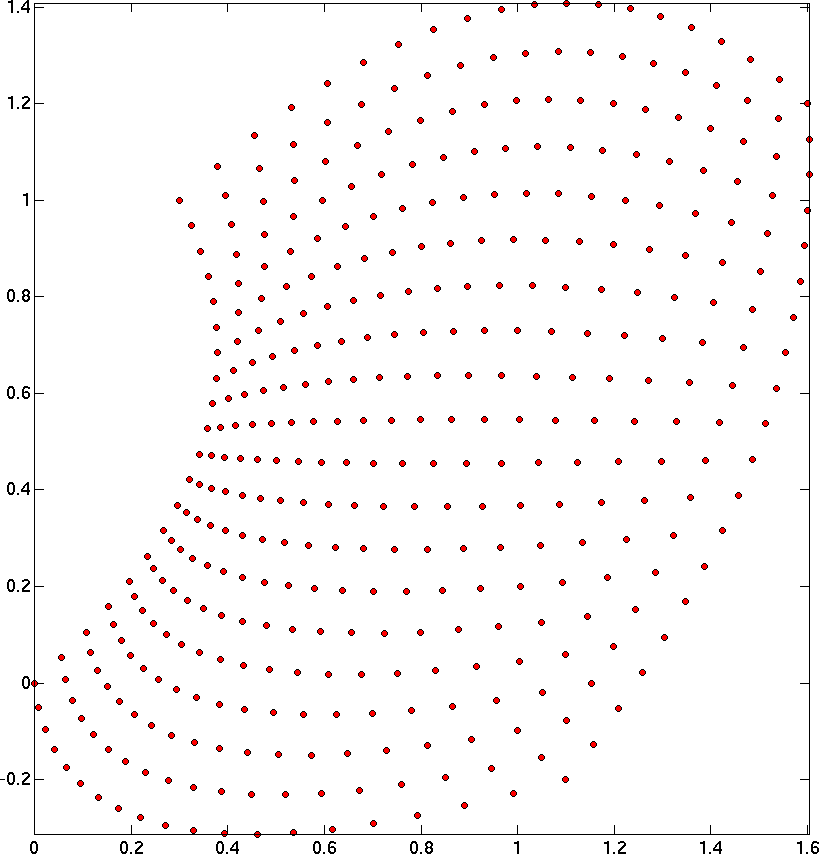
\includegraphics[height=0.4\textheight,keepaspectratio=true]{./Images/Q2Points_Physical.png}
    
    \medskip
    \tiny{\textcolor{blue}{Basis function in physical space}}
    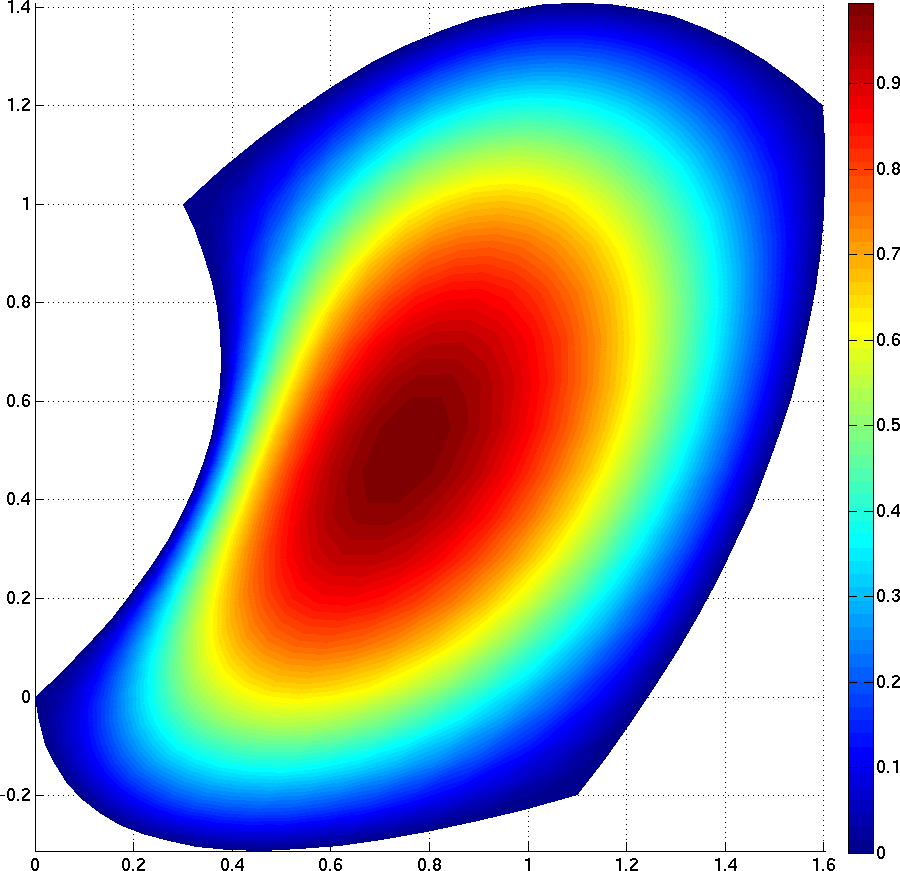
\includegraphics[height=0.4\textheight,keepaspectratio=true]{./Images/Q2Basis_Physical.png}
   \end{center}
   \end{column}
   \end{columns}
  \end{column}
 \end{columns}
\end{frame}



\begin{frame}
 \frametitle{High Order Methods Using the Q2 Basis}
 For each zone in the computational mesh, we compute the following matrices using Gauss-Legendre quadrature of a specified order.:
 \medskip
 \begin{columns}
  \begin{column}{0.3\textwidth}
   \tiny{The symmetric positive definite 9 by 9 mass matrix describes how matter is distributed within the Q2 zone}
  \end{column}
  \begin{column}{0.5\textwidth}
   \fcolorbox{black}{cyan!30}{$\displaystyle
     (\mathbf{M}_z)_{i,j}\equiv\int_{\hat{\Omega}_z} \rho_z (w_i w_j) |\mathbf{J}_z|$}
  \end{column}
 \end{columns}
 
 \bigskip
 \begin{columns}
  \begin{column}{0.3\textwidth}
   \tiny{The \textbf{rectangular} derivative matrix maps between the pressure and velocity spaces. This matrix is a discrete version of the \textbf{Div} operator. Its adjoint (transpose) is the \textbf{Grad} operator}
  \end{column}
  \begin{column}{0.5\textwidth}
   \fcolorbox{black}{cyan!30}{\parbox{4.3cm}{$\displaystyle
     (\mathbf{D}_z^x)_{i,j}\equiv\int_{\hat{\Omega}_z} \phi_i (\mathbf{J}_z^{-1}\vec{\nabla}w_j)\cdot \{1,0\} |\mathbf{J}_z|$\\
     $\displaystyle
     (\mathbf{D}_z^y)_{i,j}\equiv\int_{\hat{\Omega}_z} \phi_i (\mathbf{J}_z^{-1}\vec{\nabla}w_j)\cdot \{0,1\} |\mathbf{J}_z|$}}
  \end{column}
 \end{columns}
 
 \bigskip
 \begin{columns}
  \begin{column}{0.3\textwidth}
   \tiny{The symmetric positive definite 9 by 9 stiffness matrix is a discrete version of the second order DivGrad operator. It is used to compute the artificial viscosity}
  \end{column}
  \begin{column}{0.5\textwidth}
   \fcolorbox{black}{cyan!30}{$\displaystyle
     (\mathbf{S}_z)_{i,j}\equiv\int_{\hat{\Omega}_z} \mu_z (\mathbf{J}_z^{-1}\vec{\nabla}w_i)(\mathbf{J}_z^{-1}\vec{\nabla}w_j) |\mathbf{J}_z|$}
  \end{column}
 \end{columns}
 
 \bigskip
 The bulk of the computational effort is in computing the high order Jacobian matrix. However, this can be computed once per quadrature point and shared between each matrix.
 
 \medskip
 \begin{block}{}
  For the remaining examples, we apply \textcolor{red}{\textbf{mass lumping}} to the mass matrix to eliminate the need for a global linear solve. In addition, we compute the mass matrix only once as an initial condition.
 \end{block}


\end{frame}



\begin{frame}
 \frametitle{Static Momentum Equation Solve Convergence Study}
 \begin{columns}
  \begin{column}{0.6\textwidth}
   In this simple test, we project an analytic pressure function
    onto a randomly perturbed mesh and solve for the
    resulting accelerations:
    \begin{columns}
    \begin{column}{0.6\textwidth}
    \[
     p(x,y)=\cos(\dfrac{\pi}{2}x)\cos(\dfrac{\pi}{2}y)
    \]
    \[
     ma=-\nabla p
    \]
    \[
     \mathbf{Ma}=-\mathbf{D}^T\mathbf{p}
    \]
    \end{column}
    \begin{column}{0.4\textwidth}
    \begin{figure}[h!]
    \centering
    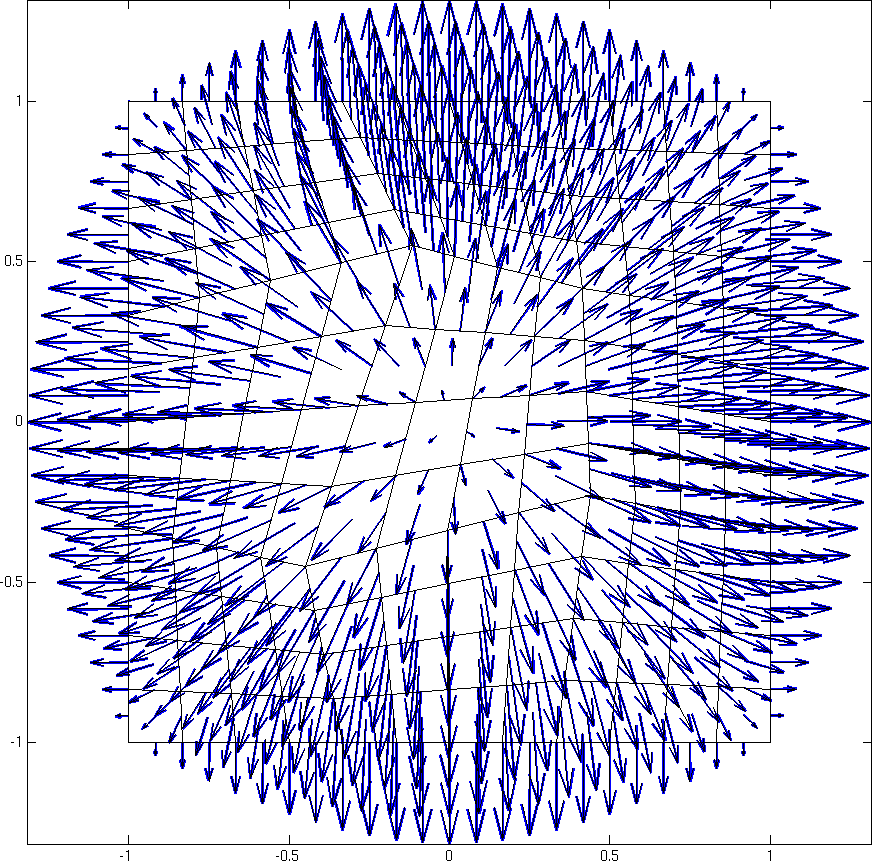
\includegraphics[width=1.0\textwidth,keepaspectratio=true]{./Images/GradPMesh_Acceleration_h2.png}
    % lagHydro.png: 434x611 pixel, 107dpi, 10.27x14.45 cm, bb=0 0 291 410
    \end{figure}
    \smallskip
    \end{column}
    \end{columns}
    Randomly perturbed base line mesh and a sequence of refinements
    \begin{columns}
    \begin{column}{0.3\textwidth}
    \begin{figure}[h!]
    \centering
    \includegraphics[width=1.0\textwidth,keepaspectratio=true]{./Images/GradPMesh_h1.png}
    % lagHydro.png: 434x611 pixel, 107dpi, 10.27x14.45 cm, bb=0 0 291 410
    \end{figure}
    \end{column}
    \begin{column}{0.3\textwidth}
    \begin{figure}[h!]
    \centering
    \includegraphics[width=1.0\textwidth,keepaspectratio=true]{./Images/GradPMesh_h2.png}
    % lagHydro.png: 434x611 pixel, 107dpi, 10.27x14.45 cm, bb=0 0 291 410
    \end{figure}
    \end{column}
    \begin{column}{0.3\textwidth}
    \begin{figure}[h!]
    \centering
    \includegraphics[width=1.0\textwidth,keepaspectratio=true]{./Images/GradPMesh_h3.png}
    % lagHydro.png: 434x611 pixel, 107dpi, 10.27x14.45 cm, bb=0 0 291 410
    \end{figure}
    \end{column}
    \end{columns}
  \end{column}
  \begin{column}{0.4\textwidth}
  \centering
  \small{Lumped mass matrix}
   \begin{figure}[h!]
    \centering
    \includegraphics[width=0.8\textwidth,keepaspectratio=true]{./Images/GradPError_Lumped.png}
    % lagHydro.png: 434x611 pixel, 107dpi, 10.27x14.45 cm, bb=0 0 291 410
  \end{figure}
  \centering
  \small{Full linear solve}
  \begin{figure}[h!]
    \centering
    \includegraphics[width=0.8\textwidth,keepaspectratio=true]{./Images/GradPError_FullMass.png}
    % lagHydro.png: 434x611 pixel, 107dpi, 10.27x14.45 cm, bb=0 0 291 410
  \end{figure}
  \end{column}
 \end{columns}

\end{frame}

% 1D Sod Shock Tube: Velocity and Density
\begin{frame}
 \frametitle{1D Sod Shock Tube: Velocity and Density}
 \begin{columns}
  \begin{column}{0.4\textwidth}
   \begin{figure}[h!]
    \centering
    \includegraphics[width=1.0\textwidth,keepaspectratio=true]{./Images/SodVelocity_Compare.png}
    % lagHydro.png: 434x611 pixel, 107dpi, 10.27x14.45 cm, bb=0 0 291 410
    \end{figure}
  \end{column}
  \begin{column}{0.4\textwidth}
   \begin{figure}[h!]
    \centering
    \includegraphics[width=1.0\textwidth,keepaspectratio=true]{./Images/SodDensity_Compare.png}
    % lagHydro.png: 434x611 pixel, 107dpi, 10.27x14.45 cm, bb=0 0 291 410
    \end{figure}
  \end{column}
 \end{columns}
 \begin{itemize}
  \item We consider two meshes: A coarse 60 zone mesh and fine 120 zone mesh
  \item For each method, $q_{lin}$ = $q_{quad}$ = 1.0, no monotonic limiter is used
  \item We acknowledge this is sub-standard for Q1 (i.e. limiters make a difference); however, this a fair comparison between each method
  \item For each zone, 5 plot points are evaluated
  \item Each method captures contact discontinuity exactly due to discontinuous thermodynamic basis
 \end{itemize}
\end{frame}

\begin{frame}
 \frametitle{1D Sod Shock Tube: Velocity and Density (Zoomed View)}
 \begin{columns}
  \begin{column}{0.4\textwidth}
   \begin{figure}[h!]
    \centering
    \includegraphics[width=1.0\textwidth,keepaspectratio=true]{./Images/SodVelocityZoom_Compare.png}
    % lagHydro.png: 434x611 pixel, 107dpi, 10.27x14.45 cm, bb=0 0 291 410
    \end{figure}
  \end{column}
  \begin{column}{0.4\textwidth}
   \begin{figure}[h!]
    \centering
    \includegraphics[width=1.0\textwidth,keepaspectratio=true]{./Images/SodDensityZoom_Compare.png}
    % lagHydro.png: 434x611 pixel, 107dpi, 10.27x14.45 cm, bb=0 0 291 410
    \end{figure}
  \end{column}
 \end{columns}
 \begin{itemize}
  \item We consider two meshes: A coarse 60 zone mesh and fine 120 zone mesh
  \item For each method, $q_{lin}$ = $q_{quad}$ = 1.0, no monotonic limiter is used
  \item We acknowledge this is sub-standard for Q1 (i.e. limiters make a difference); however, this a fair comparison between each method
  \item For each zone, 5 plot points are evaluated
  \item Each method captures contact discontinuity exactly due to discontinuous thermodynamic basis
 \end{itemize}
\end{frame}

\begin{frame}
 \frametitle{The Acoustic Wave Problem}
\begin{columns}
 \begin{column}{0.3\textwidth}
\textbf{Tests:}
  \begin{itemize}
   \item Methods independent of artificial viscosity
   \item Spurious velocity and pressure modes
   \item Correct wave speed
  \end{itemize}

\textbf{Ideally:}
\begin{itemize}
 \item Smooth waves
 \item No spurious modes
 \item Wave speed = 1
\end{itemize}

\textbf{Known Issues:}
\begin{itemize}
 \item No analytical solution
 \item Does not converge under refinement
\end{itemize}

 \end{column}
 \begin{column}{0.7\textwidth}
    \begin{figure}[h!]
    \centering
    \includegraphics[width=0.8\textwidth,keepaspectratio=true]{./Images/AcousticWave.png}
    \end{figure}
 \end{column}
\end{columns}
\end{frame}

\begin{frame}
 \frametitle{Acoustic Wave Problem: Q1-Q0}
   \begin{figure}[h!]
    \centering
    \includegraphics[width=0.8\textwidth,keepaspectratio=true]{./Images/acousticQ1Q0_hgOFF.png}
    \end{figure}
   \begin{figure}[h!]
    \centering
    \includegraphics[width=0.8\textwidth,keepaspectratio=true]{./Images/acousticQ1Q0_hgON.png}
    \end{figure}
\end{frame}

\begin{frame}
 \frametitle{Acoustic Wave Problem: Q2-Q1d}
   \begin{figure}[h!]
    \centering
    \includegraphics[width=0.8\textwidth,keepaspectratio=true]{./Images/acousticQ2Q1_hgOFF.png}
    \end{figure}
   \begin{figure}[h!]
    \centering
    \includegraphics[width=0.8\textwidth,keepaspectratio=true]{./Images/acousticQ2Q1_hgON.png}
    \end{figure}
\end{frame}

\begin{frame}
 \frametitle{Hourglass / Checkerboard Modes}
\bigskip
We define an hourglass mode to be any continuous velocity mode that
has non-zero divergence, but zero discrete divergence$^{[1]}$
\bigskip

\begin{columns}
 \begin{column}{0.6\textwidth}
\begin{columns}
\begin{column}{0.3\textwidth}
\begin{center}
 \fcolorbox{black}{cyan!30}{\Large{$\displaystyle \vec{\nabla}\cdot\vec{v}\neq 0$}}
\end{center}
\end{column}
\begin{column}{0.2\textwidth}
\begin{center}
 \includegraphics[width=.5in,keepaspectratio=true]{./Images/redLRarrow.png}
\end{center}
\end{column}
\begin{column}{0.3\textwidth}
\begin{center}
 \fcolorbox{black}{cyan!30}{\Large{$\displaystyle \mathbf{D}_z\mathbf{v}_z = 0$}}
\end{center} 
\end{column}
\end{columns}
\end{column}
\end{columns}

\bigskip
\begin{columns}
 \begin{column}{0.5\textwidth}
  \centering
   \includegraphics[height=0.5\textheight,keepaspectratio=true]{./Images/hgmodesQ1Q0.png}
 \end{column}
 \begin{column}{0.5\textwidth}
  \centering
   \includegraphics[height=0.5\textheight,keepaspectratio=true]{./Images/hgmodesQ2Q1.png}
 \end{column}
\end{columns}

\bigskip
\tiny{[1] Idea proposed by V. Dobrev and T. Kolev}
\end{frame}



\begin{frame}
 \frametitle{The Noh Implosion Problem}
\begin{columns}
 \begin{column}{0.3\textwidth}
\textbf{Tests:}
  \begin{itemize}
   \item Compression problems
   \item Symmetry preservation
   \item Artificial viscosity
   \item Shock speed
   \item Strong shocks
  \end{itemize}

\textbf{Ideally:}
\begin{itemize}
 \item Postshock density = 16
 \item Shock travels at speed of 1/3
 \item Sharp shock front
\end{itemize}

\textbf{Known Issues:}
\begin{itemize}
 \item ``Wall heating'' numerically ``heats'' the zone at the origin
\end{itemize}

 \end{column}
 \begin{column}{0.7\textwidth}
    \begin{figure}[h!]
    \centering
    \includegraphics[width=0.9\textwidth,keepaspectratio=true]{./Images/NohImplosion.png}
    % lagHydro.png: 434x611 pixel, 107dpi, 10.27x14.45 cm, bb=0 0 291 410
    \end{figure}
 \end{column}
\end{columns}
\end{frame}


\begin{frame}
 \frametitle{Noh Implosion Problem, 30 by 30 Mesh: Q1-Q0}
 \begin{columns}[T]
  \begin{column}{0.24\textwidth}
  \bigskip
   \begin{itemize}
   \small{
%     \item No HG filter required
    \item Shock is not well resolved on this coarse mesh
    \item No overshoots or undershoots are observed}
   \end{itemize}
  \end{column}
  \begin{column}{0.8\textwidth}
   \begin{figure}[h!]
    \centering
    \includegraphics[width=0.9\textwidth,keepaspectratio=true]{./Images/NewNoh_Q1Q0.png}
    % lagHydro.png: 434x611 pixel, 107dpi, 10.27x14.45 cm, bb=0 0 291 410
    \end{figure}
  \end{column}
 \end{columns}
\end{frame}

\begin{frame}
 \frametitle{Noh Implosion Problem, 30 by 30 Mesh: Q2-Q1d}
 \begin{columns}[T]
  \begin{column}{0.24\textwidth}
  \bigskip
   \begin{itemize}
   \tiny{
%     \item No HG filter used
    \item 36 plot points per zone
    \item Shock is more sharply resolved
    \item Wall heating is diminished
    \item Post shock density is closer to correct value
    \item Strong undershoots and overshoots in the density are observed in the single layer of zones at shock front
    }
   \end{itemize}
  \end{column}
  \begin{column}{0.8\textwidth}
   \begin{figure}[h!]
    \centering
    \includegraphics[width=0.9\textwidth,keepaspectratio=true]{./Images/NewNoh_Q2Q1.png}
    % lagHydro.png: 434x611 pixel, 107dpi, 10.27x14.45 cm, bb=0 0 291 410
    \end{figure}
  \end{column}
 \end{columns}
\end{frame}

% \begin{frame}
%  \frametitle{Noh Implosion Problem, 30 by 30 Mesh: Q2-Q2d FEM}
%  \begin{columns}[T]
%   \begin{column}{0.24\textwidth}
%   \bigskip
%    \begin{itemize}
%    \tiny{
%     \item No HG filter used
%     \item 36 plot points per zone
%     \item Shock is more sharply resolved
%     \item Wall heating is diminished
%     \item Post shock density is closer to correct value
%     \item Under shoots in density diminished, but overshoots persist
%     }
%    \end{itemize}
%   \end{column}
%   \begin{column}{0.8\textwidth}
%    \begin{figure}[h!]
%     \centering
%     \includegraphics[width=0.9\textwidth,keepaspectratio=true]{./Images/NewNoh_Q2Q2.png}
%     % lagHydro.png: 434x611 pixel, 107dpi, 10.27x14.45 cm, bb=0 0 291 410
%     \end{figure}
%   \end{column}
%  \end{columns}
% \end{frame}

\begin{frame}
 \frametitle{The Saltzman Piston Problem}
\begin{columns}[t]
 \begin{column}{0.3\textwidth}
\textbf{Tests:}
  \begin{itemize}
   \item Artificial viscosity
   \item Shocks that are not aligned with the mesh
   \item Shock-mesh interaction
   \item Mesh tangling
  \end{itemize}
 \end{column}
 \begin{column}{0.3\textwidth}
\textbf{Ideally:}
  \begin{itemize}
   \item Post-shock density = 20
   \item Pre-shock density = 10
   \item Shock line is vertical
   \item Horizontal mesh lines stay that way
  \end{itemize}
 \end{column}
 \begin{column}{0.3\textwidth}
\textbf{Known Issues:}
  \begin{itemize}
   \item ``Wall heating'' at both ends
  \end{itemize}
 \end{column}
\end{columns}
    \begin{figure}[h!]
    \centering
    \includegraphics[width=0.9\textwidth,keepaspectratio=true]{./Images/SaltzmanPiston.png}
    % lagHydro.png: 434x611 pixel, 107dpi, 10.27x14.45 cm, bb=0 0 291 410
    \end{figure}
\begin{center}
Simulation will run till t = 0.925
\end{center}
\end{frame}

\begin{frame}
 \frametitle{Saltzman Piston Problem, 50 by 10 Mesh: Q1-Q0}
   \begin{figure}[h!]
    \centering
    \includegraphics[width=\textwidth,keepaspectratio=true]{./Images/Saltzman_Q1Q0.png}
    \end{figure}
\end{frame}

% \begin{frame}
%  \frametitle{Saltzman Piston Problem, 50 by 10 Mesh: Q1-Q1d}
%    \begin{figure}[h!]
%     \centering
%     \includegraphics[width=\textwidth,keepaspectratio=true]{./Images/Saltzman_Q1Q1.png}
%     \end{figure}
% \end{frame}

\begin{frame}
 \frametitle{Saltzman Piston Problem, 50 by 10 Mesh: Q2-Q1d}
   \begin{figure}[h!]
    \centering
    \includegraphics[width=\textwidth,keepaspectratio=true]{./Images/Saltzman_Q2Q1.png}
    \end{figure}
\end{frame}

% \begin{frame}
%  \frametitle{Saltzman Piston Problem, 50 by 10 Mesh: Q2-Q2d}
%    \begin{figure}[h!]
%     \centering
%     \includegraphics[width=\textwidth,keepaspectratio=true]{./Images/Saltzman_Q2Q2.png}
%     \end{figure}
% \end{frame}

\begin{frame}
 \frametitle{The Sedov Explosion Problem}
\begin{columns}
 \begin{column}{0.3\textwidth}
\textbf{Tests:}
  \begin{itemize}
   \item Expansion problems
   \item Curved phenomena
   \item Correct maximum density
  \end{itemize}

\textbf{Ideally:}
\begin{itemize}
 \item Maximum density = 6
 \item Circular shock
 \item Curved zones close to analytical mesh
 \item Sharp shock front
 \item No velocity oscillations
\end{itemize}

\textbf{Known Issues:}
\begin{itemize}
 \item Hourglass modes render $Q_1-Q_0$ solution impossible without filter
\end{itemize}

 \end{column}
 \begin{column}{0.7\textwidth}
    \begin{figure}[h!]
    \centering
    \includegraphics[width=0.8\textwidth,keepaspectratio=true]{./Images/SedovExplosion.png}
    % lagHydro.png: 434x611 pixel, 107dpi, 10.27x14.45 cm, bb=0 0 291 410
    \end{figure}
 \end{column}
\end{columns}
\end{frame}

\begin{frame}
 \frametitle{Sedov Explosion Problem, 20 by 20 Mesh: Q1-Q0}
 \begin{columns}[T]
  \begin{column}{0.24\textwidth}
  \bigskip
   \begin{itemize}
   \small{
    \item Standard HG filter required
    \item Shock is not well resolved on this coarse mesh
    \item Zone at origin has straight edges}
   \end{itemize}
  \end{column}
  \begin{column}{0.8\textwidth}
   \begin{figure}[h!]
    \centering
    \includegraphics[width=0.9\textwidth,keepaspectratio=true]{./Images/NewSedov_Q1Q0.png}
    % lagHydro.png: 434x611 pixel, 107dpi, 10.27x14.45 cm, bb=0 0 291 410
    \end{figure}
  \end{column}
 \end{columns}
\end{frame}

\begin{frame}
 \frametitle{Sedov Explosion Problem, 20 by 20 Mesh: Q2-Q1d}
 \begin{columns}[T]
  \begin{column}{0.24\textwidth}
  \bigskip
   \begin{itemize}
   \tiny{
    \item No HG filter used
    \item Curved elements
    \item 81 plot points used per cell
    \item Shock front is much sharper on the same mesh
    \item Zone at origin has incorrect deformation
    \item Velocity oscillations are observed in post shock region
    }
   \end{itemize}
  \end{column}
  \begin{column}{0.8\textwidth}
   \begin{figure}[h!]
    \centering
    \includegraphics[width=0.9\textwidth,keepaspectratio=true]{./Images/NewSedov_Q2Q1.png}
    % lagHydro.png: 434x611 pixel, 107dpi, 10.27x14.45 cm, bb=0 0 291 410
    \end{figure}
  \end{column}
 \end{columns}
\end{frame}

\begin{frame}
 \frametitle{Sedov Explosion Problem, 20 by 20 Mesh: Q2-Q1d}
 \begin{columns}[T]
  \begin{column}{0.24\textwidth}
  \bigskip
   \begin{itemize}
   \tiny{
    \item No HG filter used
    \item 81 plot points used per cell
    \item Allowing 25\% of the linear-q term in expansion has a significant benefit
    \item Velocity oscillations in post shock region are eliminated
    \item Curved deformation of zones closely resembles exact deformation
    \item We have not taken full benefit of the high order information in each cell to compute the viscosity coefficient, this is an area we plan to investigate much further
    }
   \end{itemize}
  \end{column}
  \begin{column}{0.8\textwidth}
   \begin{figure}[h!]
    \centering
    \includegraphics[width=0.9\textwidth,keepaspectratio=true]{./Images/NewSedov_Q2Q1Mod.png}
    \end{figure}
  \end{column}
 \end{columns}
\end{frame}

\begin{frame}
 \frametitle{Sedov Explosion Problem, 20 by 20 Mesh Comparison}
 \begin{figure}[h!]
  \centering
  \includegraphics[width=1.0\textwidth,keepaspectratio=true]{./Images/SedovCompare.png}
  \end{figure}
\end{frame}

\begin{frame}
 \frametitle{Sedov Explosion Problem, Full Mesh Comparison}
\begin{itemize}
 \item High order methods naturally represent curved zones
 \item Low order methods lack the flexibility to model curved phenomena
 \begin{itemize}
  \item Simulation crashes at t = 0.868
 \end{itemize}
\end{itemize}

 \begin{figure}[h!]
  \centering
  \includegraphics[width=1.0\textwidth,keepaspectratio=true]{./Images/SedovFullMeshCompare.png}
  \end{figure}
\end{frame}

\begin{frame}
 \frametitle{Other Elements Considered: Q1-Q1d}
 \begin{columns}[T]
\begin{column}{0.02\textwidth}
\end{column}
  \begin{column}{0.24\textwidth}
  \bigskip
\textbf{Noh:}
   \begin{itemize}
    \item More stable than Q1-Q0
    \item Less accurate than Q2-Q1d
   \end{itemize}
\textbf{Saltzman:}
   \begin{itemize}
    \item Straighter shock than Q1-Q0
    \item Wavy horizontal mesh lines
   \end{itemize}
\textbf{Sedov:}
   \begin{itemize}
    \item More circular shock than Q1-Q0
    \item Better maximum density than Q1-Q0
    \item Does not require hourglass filter
    \item Straight-edged zones
   \end{itemize}
  \end{column}
  \begin{column}{0.8\textwidth}
   \begin{figure}[h!]
    \centering
    \includegraphics[width=0.9\textwidth,keepaspectratio=true]{./Images/Sedov_Q1Q1_10x10.png}
    \end{figure}
  \end{column}
 \end{columns}
\end{frame}

\begin{frame}
 \frametitle{Other Elements Considered: Q2-Q2d}
 \begin{columns}[T]
\begin{column}{0.02\textwidth}
\end{column}
  \begin{column}{0.24\textwidth}
  \bigskip
\textbf{Noh:}
   \begin{itemize}
    \item Limites density undershoots
    \item Exacerbates density overshoots
   \end{itemize}
\textbf{Saltzman:}
   \begin{itemize}
    \item Runs without hourglass filter
    \item Inferior to Q2-Q1d
   \end{itemize}
\textbf{Sedov:}
   \begin{itemize}
    \item Spurious oscillations
    \item Negatively curved zones
    \item Requires hourglass filter
    \item More accurate than low order methods
   \end{itemize}
  \end{column}
  \begin{column}{0.8\textwidth}
   \begin{figure}[h!]
    \centering
    \includegraphics[width=0.9\textwidth,keepaspectratio=true]{./Images/Noh_Q2Q2_30x30.png}
    \end{figure}
  \end{column}
 \end{columns}
\end{frame}


\begin{frame}
 \frametitle{Computational Efficiency}
\begin{itemize}
 \item Low order methods require $2^{nD}$ elements for comparable accuracy
 \item Many calculations are done zone-by-zone
 \item Putting more of the computational burden on each zone increases computational efficiency
\end{itemize}

\begin{block}{High order element speedup}
\begin{center}
\begin{tabular}[c]{|c|cc|cc|cc|}
\hline
\multicolumn{7}{|c|}{\textbf{Sedov Explosion Problem}} \\
\hline
Method & \multicolumn{2}{|c|}{36 Degrees of Freedom} & \multicolumn{2}{|c|}{121 Degrees of Freedom} & \multicolumn{2}{|c|}{441 Degrees of Freedom}\\
\hline
 & Run Time & Speedup & Run Time & Speedup & Run Time & Speedup\\
$Q_1-Q_0$ & 28.154 & 1.0 & 156.021 & 1.0 & 1265.232 & 1.0 \\
$Q_1-Q_{1d}$ & 29.565 & 0.95 & 165.185 & 0.94 & 1291.628 & 0.98 \\
$Q_2-Q_{1d}$ & 16.328 & 1.72 & 73.375  & 2.13 & 623.658 & 2.03 \\
$Q_2-Q_{2d}$ & 17.017 & 1.65 & 77.632  & 2.01 & 663.122 & 1.91 \\
\hline
\multicolumn{7}{c}{} \\
\hline
\multicolumn{7}{|c|}{\textbf{Noh Implosion Problem}} \\
\hline
Method & \multicolumn{2}{|c|}{36 Degrees of Freedom} & \multicolumn{2}{|c|}{121 Degrees of Freedom} & \multicolumn{2}{|c|}{441 Degrees of Freedom}\\
\hline
 & Run Time & Speedup & Run Time & Speedup & Run Time & Speedup\\
$Q_1-Q_0$    & 101.192 & 1.0 & 383.356 & 1.0 & 1543.319 & 1.0 \\
$Q_1-Q_{1d}$ & 103.048 & 0.98 & 396.967 & 0.97 & 1590.766 & 0.97 \\
$Q_2-Q_{1d}$ & 53.042 & 1.91 & 191.063  & 2.01 & 775.230 & 1.99 \\
$Q_2-Q_{2d}$ & 53.605 & 1.89 & 194.381  & 1.97 & 792.363 & 1.95 \\
\hline
\end{tabular}
\end{center}
\end{block}

\end{frame}


\begin{frame}
 \frametitle{Conclusions}
 We have developed a general FEM framework for Lagrangian CFD
 \begin{itemize}
 \item Kinematic and thermodynamic space can be chosen independently
 \item For triangles:
 \begin{itemize}
 \item Linear, quadratic, cubic, etc. kinematic space
 \item Constant, linear, quadratic, etc. thermodynamic space
 \end{itemize}
 \item For quads:
 \begin{itemize}
 \item Bi-linear, bi-quadratic, bi-cubic, etc. kinematic space
 \item Constant, bi-linear, bi-quadratic, etc. thermodynamic space
 \end{itemize}
 \item This allows us to experiment with many different finite element pairs

 \end{itemize}

 We have also demonstrated that high order Lagrangian methods have significant promise
 \begin{itemize}
  \item  Permits curved elements
  \item  Increased accuracy
  \item  Sharper shocks
  \item  Density/pressure gradients in a single cell
  \item  Second derivatives of velocity in a single cell
  \item  Potential improvements for sub-zonal physics / multi-material ALE
  \item  Post shock ringing is still an issue and we plan to address this by improving the artificial viscosity coefficient (e.g. the Hyper Viscosity technique of Cook and Cabot)
  \item More computationally efficient
 \end{itemize}
\end{frame}

\begin{frame}
 \frametitle{Questions?}
\begin{figure}[h!]
 \centering
 \includegraphics[width=1.0\textwidth,keepaspectratio=true]{./Images/SedovCombined.png}
 % Questions.png: 848x409 pixel, 90dpi, 23.94x11.55 cm, bb=0 0 679 327
\end{figure}
\end{frame}

\end{document}